\ProvidesFile{thesis.tex}[2021-08-23 PurdueThesis template file]

%
%  Be sure to sign up for the PurdueThesis mailing list at
%      https://engineering.purdue.edu/ECN/mailman/listinfo/purduethesis-list
%  so you learn of new versions of this software.  You must be
%  on that mailing list to receive help with this software.
%
%  Process this using lualatex instead of pdflatex because of the
%  Feynman diagrams in the "Physics" appendix.
%
%  This is the root file for a simple example thesis.
%  This example can also be used to prepare a dissertation.
%
%  This thesis contains Feynman diagrams in the ap-physics.tex file.
%  For these to be processed correctly you must use the lualatex
%  program.  If your thesis doesn't have Feynman diagrams use pdflatex
%  instead of lualatex.
%  To make a final copy of your thesis put a '%'
%  in front of the \includeonly command and run:
%    lualatex thesis
%    lualatex thesis
%    lualatex thesis
%    biber thesis
%    makeindex thesis
%    lualatex thesis
%    lualatex thesis
%  Running Overleaf on your thesis file should do all of this
%  automatically.
%
%  References cited below:
%
%    TM2017 is short for Thesis Manual 2017:
%        A Manual for the Preparation of Graduate Theses,
%        eighth revised edition,
%        Thesis and Dissertation Office,
%        Purdue University,
%        2017,
%        revised August 30, 2017,
%        http://www.purdue.edu/gradschool/documents/thesis/graduate-thesis-manual.pdf,
%        last retrieved on May, 8, 2021.
%
%  Search for ``CHANGE'' below and change things as necessary.
%  I recommend putting ``%%'' before any existing lines that
%  need to be changed and adding your new line(s) immediately
%  below the existing lines.
%



% institution
% Choose an institution name from the following list:
%     VALUE                   COMMENT
%     Purdue University
%     University of Hawaii    don't include the 'okina character here,
%                             it will get printed automatically
\def\ZZinstitution{Purdue University}


% campus
% Choose a campus from the following list:
%     VALUE           COMMENT
%     Bloomington
%     Fort Wayne
%     Hammond
%     Indianapolis
%     Manoa           don't include the macron character here,
%                     it will get printed automatically
%     Reno
%     Westville                 
%     West Lafayette
\def\ZZcampus{West\space Lafayette}


% program
% Choose a program from the following list:
%     Chemistry
\def\ZZprogram{Chemistry}


% degree
% Choose a degree from the following list:
%     Doctor of Philosophy
\def\ZZdegree{Doctor of Philosophy}

% author
% Put your name here.
\def\ZZauthor{Armen Beck}

% document
% Choose a document from the following list:
%     A Dissertation
%     A Master's Bypass Report
%     A Preliminary Report
%     A Thesis
\def\ZZdocument{A Dissertation}

% graduation
% Chose a month from
%     May
%     August
%     December
% followed by a space
% then choose a year from 2020 to 2030.
\def\ZZgraduation{August 2023}

% title
% If you need to manually split the title,
% over several lines do, for example,
%     \def\ZZtitle{%
%       This is the First Line\\[-6pt]
%       and this is the Second Line%
%     }
\def\ZZtitle{Bit by Bit Chemistry: Data Driven Software for Chemical Systems}

% showdiagonalline
% Show a diagonal line from lower left to center
% of main printed part of page?
% THE SUBMITTED COPY OF YOUR THESIS MUST BE RUN WITH diagonalline = {false}.
\def\ZZshowdiagonalline{false}

% showgridlines
% Show grid lines on main printed part of page
% Vertical and horizontal grid lines are put
% in the normal printed part of the page---this
% includes lines where the margins are.
% THE SUBMITTED COPY OF YOUR THESIS MUST BE RUN WITH gridlines = {false}.
\def\ZZshowgridlines{false}

% showmarginlines
% Show margin lines on the edge of the normal printed part of the page?
% Margin lines show where the margins are.
% THE SUBMITTED COPY OF YOUR THESIS MUST BE RUN WITH marginlines = {false}.
%     VALUE    MEANING
%     false    don't show marginlines
%     true     show marginlines
\def\ZZshowmarginlines{false}

% showtimestamp
% Show, for example, a "compiled on  2021-03-02  Tuesday  17:16:24"
% timestamp in the upper right corner of page?
%     VALUE    MEANING
%     false    don't show timestamp
%     true     show timestamp
% THE SUBMITTED COPY OF YOUR THESIS MUST BE RUN WITH timestamp = {false}.
\def\ZZshowtimestamp{false}

% todonotes
% Set things up for todonotes.
%     VALUE    MEANING
%     false    don't put todo notes in PDF file
%     true     put 0.8 inch wide todo notes in PDF file
%     wide     put 3.8 inch wide todo notes in PDF file, do not send
%              todonotes = wide output to a printer
% THE SUBMITTED COPY OF YOUR THESIS MUST BE RUN WITH todonotes = {false}.
\def\ZZtodonotes{false}

\documentclass{PurdueThesis}


%%%% \ExplSyntaxOn                         %%%% changed 2021-07-27 by mark
%%%% \bool_set_true:N \ZZCenterCaptionB    %%%% changed 2021-07-27 by mark
%%%% \ExplSyntaxOff                        %%%% changed 2021-07-27 by mark

\def\ZZatinformation{}
% If you are at the Hammond or Westville campus
% remove the "%" from the begining of the next line.
%\def\ZZatinformation{~at~Purdue~Northwest}

% If the title contains commas, do, for example,
% \def\ZZtitle{WIRELESS POWER TRANSFER:
% EFFICIENCY, FAR FIELD, DIRECTIVITY, AND PHASED ARRAY ANTENNAS}                  



% PurdueThesis.cls loads the rotating package which loads the graphicx
% package.  From page 12 of "Packages in the `graphics' bundle", 2021-03-05,
% retrieved 2021-06-16, at https://texdoc.org/serve/grfguide.pdf/0
%     \graphicspath{<dir-list>}
%
%         This optional declaration may be used to specify a list of
%         directories in which to search for graphics files.  The
%         format is the same as for the LaTeX 2e primitive \input@path.
%         A list of directories, each in a {} group (even if there is
%         only one in the list).  For example:
%             \graphicspath{{eps/}{tiff/}}
%         would cause the system to look in the subdirectories eps and
%         tiff of the current directory.  (All modern TeX systems use /
%         as the directory separator, even on Windows.)
%
%         The default setting of this path is \input@path that is:
%         graphics files will be found whereever TeX files are found.
%
% Look in the "graphics" subfolder for graphics files.
% This is done to reduce the number of files in the main thesis folder
% so the ones in there are easier to find.
\graphicspath{{graphics/}}

% Look in the "packages" subfolder for packages.
% This is done to reduce the number of files in the main thesis folder
% so the ones in there are easier to find.
\makeatletter
    \def\input@path{{packages/}}
\makeatother

%
% Configure bibliography.
%
% Automatically configure the bibliography.  Based on the
% institution, campus, and program listed in the \documentclass
% command \bibprocessor is set to "biblatex" or "bibtex".
% For biblatex, a
%    \usepackage[...]{biblatex}
% is done.  Put your bibliography entries in all-biblatex.bib.
% For bibtex, a
%     \bibliographystyle{...}
% command is done.  Put your bibliography entries in all-bibtex.bib.
%
% All combinations of institution, campus, and program use biblatex.
% Exceptions that use bibtex:
%     o  "Purdue University", "West Lafayette", "Earth, Atmospheric,
%        and Planetary Sciences" uses the ametsoc2014 bibliography style.
%     o  "Purdue University", "West Lafayette", "Veterinary Clinical
%        Sciences" uses the ama bibliography style.
%
% To override the default choices picked by \ConfigureBibliography, change,
% for example,
%     \ConfigureBibliography
% to
%     % \ConfigureBibliography
%     \newcommand{\bibprocessor}{biblatex}
%     \usepackage[backend=biber, citestyle=apa, dashed=false, sortcites=true, style=apa]{biblatex}
%     \addbibresource{all-biblatex.bib}
\ConfigureBibliography

%
% This is only relevant if you are using biblatex.
%
% This is an example of how to ignore urldate fields in your .bib file.
% See the first complete example on page 201 of
%     https://mirrors.rit.edu/CTAN/macros/latex/contrib/biblatex/doc/biblatex.pdf
%
% If you don't want to ignore urldate fields,
% comment out (put "%" before) the next ten lines.
%
\ifthen{\equal{biblatex}{\bibprocessor}}
{
  \DeclareSourcemap{
    \maps[datatype=bibtex]{
      \map{
        \step[fieldset=urldate, null]
      }
    }
  }
}

% To let {\bfseries\scshape text} work as expected.
% See
%     https://tex.stackexchange.com/questions/27411/small-caps-and-bold-face
\usepackage{bold-extra}

% For chemical figures.
\usepackage{chemfig}

% For typesetting cryptography pseudocode, algorithms, and protocols.
% See
%     https://mirror.las.iastate.edu/tex-archive/macros/latex/contrib/cryptocode/cryptocode.pdf
\usepackage
[
  n,            % or lambda
  advantage,
  operators,
  sets,
  adversary,
  landau,
  probability,
  notions,
  logic,
  ff,
  mm,
  primitives,
  events,
  complexity,
  oracles,
  asymptotics,
  keys,
]
{cryptocode}

% Define
%    \VerbatimInput[options]{filename}
%    \begin{VerbatimOut}{filename} ... \end{VerbatimOut}.
\usepackage{fancyvrb}
  \DefineShortVerb{\|}  % so "|verbatim|" will be verbatim

% For nlui testing.
\usepackage{listings}
  
% For chemical equations.
% See
%     https://ctan.org/pkg/mhchem?lang=en
% From the "Package documentation" linked-to document
%     mhchem needs a couple of other packages.
%     For instance, expl3, amsmath and calc.
\usepackage[version=4]{mhchem}
  % If I'm loading the package to just define a few new commands I'll indent
  % two spaces right after loading the package and define the few new
  % commands here.  If I'm defining more than a few commands I usually do it
  % after loading all the packages.
  % Define "\nitrate" to be the chemical symbol for nitrate.
  \newcommand{\nitrate}{\ce{NO3{-}}}
  % Define "\pnitrate" (short for "parenthesized nitrate") to be the chemical
  % symbol for nitrate surrounded by parentheses.
  \newcommand{\pnitrate}{(\nitrate)}
  % "Define \vpnitrate" (short for "verbose parenthesized nitrate") to be
  % the word "nitrate" followed by a space followed by the chemical symbol
  % for nitrate with parentheses around it.
  \newcommand{\vpnitrate}{nitrate (\nitrate)}

% For
%     \cancel  
%     \highlight
% See
%     http://ftp.math.purdue.edu/mirrors/ctan.org/macros/latex/contrib/siunitx/siunitx.pdf
% pages 11--12.  
\usepackage{cancel}


% Redefine description, enumerate, and itemize lists.
% See
%     https://mirrors.concertpass.com/tex-archive/macros/latex/contrib/enumitem/enumitem.pdf
% \usepackage{enumitem}
% \setlist[itemize]{leftmargin=7pt,rightmargin=24pt}


  
% This gets rid of
%     [5] (./thesis.toc
%     ! Undefined control sequence.
%     \vbox_set:Nn ...box:D {\color_group_begin: #2\par 
%                                                       \color_group_end: }
%     l.32 ...}Basic Circuit Components}{31}{section.67}
%                                                       %
%     ? 
% and
%     [6]
%     ! Undefined control sequence.
%     \vbox_set:Nn ...box:D {\color_group_begin: #2\par 
%                                                       \color_group_end: }
%     l.61 ...rline {P.1}Frenchspacing}{67}{section.445}
%                                                       %
%     ?
% errors.
% See
%     https://github.com/latex3/latex2e/issues/73
\usepackage{etoc}

% Define \setmaxprintline{number_of_columns}.
% \usepackage{hardwrap}

% For indexing.  Making an index is optional.
% Make these commands available:
%     COMMAND           DESCRIPTION
%     \index{string}    put "string" in index information
%     \makeindex        save information to make the index
%     \printindex       print the index
% See
%     https://ctan.org/pkg/makeidx?lang=en
% for more information.
\usepackage{makeidx}
  % By default \index ignores its argument.
  % This activates indexing.
  \makeindex
  % The "chapter name" for the index.
  \renewcommand{\indexname}{INDEX}

% The mathtools package
% (see http://mirror.utexas.edu/ctan/macros/latex/required/amsmath/amsmath.pdf)
% loads the amsmath package which defines the
%     align
%     align*
%     alignat
%     alignat*
%     equation
%     equation*
%     flalign
%     flalign*
%     gather
%     gather*
%     multitaper
%     multitaper*
%     split
% environments and extends amsmath by defining many other commands.
% See
%     https://ctan.org/pkg/amsmath
% for information about amsmath and
%     http://ctan.math.washington.edu/tex-archive/macros/latex/contrib/mathtools/mathtools.pdf
% for information about mathtools.
\usepackage{mathtools}

% Define \includemedia.
\usepackage{media9}

% Define \begin{multicols}{number_of_columns} ... \end{multicolumns}.
% Used in ap-text.tex.
\usepackage{multicol}

% Define \ditto.
\usepackage{pa-ditto}

% Define \FigureDash.
% \FigureDash is a dash the width of a digit in the current font.
\usepackage{pa-figure-dash}

% For PurdueThesis, PuTh, TeX, LaTeX, METAFONT, METAPOST, etc. related logos.
\usepackage{pa-logos}

% (Or maybe use isomath instead?  -mark  2021-06-20)
% Follow ISO 80000-2:2019
%     o   put e, i, and pi in upright font automatically
%     o   use, for example, "\di x" to get "\,mathrm{d}\/x"
% This loads
%     o   amsmath.sty (which is already loaded above)
%     o   mathtools.sty
%     o   upgreek.sty
% Load the package.
\usepackage{pa-mismath}
  % Tell mismath that e, i, j, and pi in upright font automatically.
  \enumber
  \inumber
  \jnumber
  \pinumber
  % To typeset math italic e, i, j, and pi use
  %     \mathit e
  %     \mathit i
  %     \mathit j
  %     \itpi

% Define \MyRepeat{what}{repeat}.
% Do "what" "repeat" number of times.
\usepackage{pa-repeat}

% Define \FloatBarrier.
% \FloatBarrier process all unproccesed floats (tables, figures, etc.).
\usepackage{placeins}

% Define \textcent.
\usepackage{textcomp}
  
% !!! This doesn't work yet, figure it out later.
% For \textprimstress.
% \usepackage{tipa}

% Needed for chapter "Graphics", section "TikZ and PGF".
\usepackage{tikz}
  % For electrical diagrams.
  % Uses the TikZ package.
  % The circuitikz name is short for "circuit TikZ".
  \usepackage{circuitikz}
  %
  \usepackage{menukeys}
  %
  % Needed for pa-typographic-conventions package.
  \usetikzlibrary{calc,shapes.symbols,shadows}
  %
  % Draw TikZ decorations.
  % Needed for at least the Kalman filter system model graphic.
  \usetikzlibrary{decorations.pathmorphing} % noisy shapes
  %
  % Fit shapes to coordinates.
  % Needed for at least the Kalman filter system model graphic.
  \usetikzlibrary{fit}
  %
  % Draw the background after the foreground.
  \usetikzlibrary{backgrounds}	% drawing the background after the foreground

% Needed for the Feynman diagram in ap-physics.tex.
% Tikz-feynman requires LuaLaTeX instead of pdflatex be run.
% LuaLaTeX screws up spacing in the list of figures so this
% is not loaded and LuaLaTeX should not be used.
\usepackage[compat=1.1.0]{tikz-feynman}

% The vertical space between a table heading and the table contents
% in a tabular environment.
\newcommand{\tabularspace}{\noalign{\vspace*{2pt}}}

% For \sfrac, used to do slanted fractions, similar to, e.g., 1/2,
% but 1 is small and high and 2 is small and low.
\usepackage{xfrac}


% Define \I.
% \I1 does \indent once, \I2 does \indent twice, etc.
\newcommand{\I}[1]{\MyRepeat{\indent}{#1}}

% Define \MyI.
% Typeset my input.
\long\def\MyI#1%
{%
  {%
    \fontsize{8}{10}\tt
    \VerbatimInput[
      firstnumber = 1,
      numbers     = left,
      xleftmargin = 0.33in,
    ]{#1}
  }%
}  

% Define \MyIO.
% Typeset my input and output.
% The input will all be on the same page.
% The output may be split over multiple pages.
\newcommand{\MyIO}
{%
  \input{z.out}

  {%
    \fontsize{8}{10}\tt
    \VerbatimInput[
      firstnumber = 1,
      numbers     = left,
      xleftmargin = 0.33in,
    ]{z.out}
  }
  \FloatBarrier
}  

% Define \MyIOS.
% Typeset my input and output.
% The input may be split over multiple pages.
% The output may be split over multiple pages.
% This doesn't work right:
%     o  Putting a \vbox around the input and output
%        does not allow todoindex entries to be listed.
%     o  Using \vfilneg at beginning and end of definition
%        screws up vertical spacing.
% \newcommand{\MyIOS}
% {%
%   \input{z.out}
% 
%   {%
%     \fontsize{8}{10}\tt
%     \VerbatimInput
%     [
%       firstnumber = 1,
%       numbers     = left,
%       xleftmargin = 0.33in,
%     ]{z.out}%
%   }
% }  

% Define \MyIOT.
% Typset my input and output together on the same page.
% This doesn't work right:
%     o  Putting a \vbox around the input and output
%        does not allow todoindex entries to be listed.
%     o  Using \vfilneg at beginning and end of definition
%        screws up vertical spacing.
% \def\MyIOT
% {%
%   \vfilneg
%   % \vbox
%   {%
%     \input{z.out}%
%     \fontsize{8}{10}\tt
%     \VerbatimInput[
%       firstnumber = 1,
%       numbers     = left,
%       xleftmargin = 0.33in,
%     ]{z.out}%
%   }%
%   \FloatBarrier
%   \vfilneg
% }  

% Define \NL (newline) so LaTeX goes to the next output line.
% Just doing \\ complains
%     ! LaTeX Error: There's no line here to end.
% \mbox{} is an empty math box.
\newcommand{\NL}{\mbox{}\\}

% Print a list of files used and their version numbers in the log file.
\listfiles


% \def\bibindent{0em}
% Customize the bibliography.
% \DefineBibliographyStrings{english}{
%   urlfrom = {URLFROM},
%   urlseen = {URLSEEN}
% }

\usepackage{url}
\usepackage{hyperref}

% For typographical conventions stuff including
%     \Emph{...}
%     \First{...}
%     \Keys{...}
%     \Literal{...}
%     \Menu{...}
%     \Place{...}
%     \Shell{...}
%%%% This must be after
%%%%     \usepackage{tikz}
\usepackage{pa-typographic-conventions}

\usepackage{tabularray}
\usepackage{multirow}
\usepackage{longtable}
\usepackage{xcolor,colortbl}
\usepackage{nicematrix}
\usepackage{makecell} 
\usepackage{array}
\newcolumntype{?}{!{\vrule width 1pt}}
\begin{document}

\NiceMatrixOptions
  {
    custom-line = 
     {
       letter = I , % for the vertical rules
       command = boldhline , % the horizontal rules 
       total-width = 1 pt , 
       tikz = { line width = 1 pt } 
     }
  }
  

\maketitle

% Define front matter
%     dedication
%     acknowledgments
%     preface
%     table of contents
%     list of tables
%     list of figures
%     list of symbols
%     abbreviations
%     nomenclature
%     glossary
%     abstract
\ProvidesFile{ch-front.tex}[2021-08-23 front matter chapter]
%
%  This is ``front matter'' for the thesis.
%
%  REFERENCES
%
%    TCMOS17
%      The Chicago Manual of Style Online, 17th edition.
%      https://www.chicagomanualofstyle.org/home.html
%      retrieved on 2020-02-29
%
%    TEMPL
%      Thesis and Disertation Office Templates.
%      https://www.purdue.edu/gradschool/research/thesis/templates.html
%      retrieved on 2020-02-29
%
%    WNNCD
%    Webster's Ninth New Collegiate Dictionary.
%

%
%   Only Purdue University uses this page
%
%   Comment out \begin{statement} through \end{statement}
%   if you are not at Purdue University.
%
% Statement of Thesis/Dissertation Approval Page
% This page is REQUIRED.  The page should be numbered "2"
% and should NOT be listed in your TABLE OF CONTENTS.
\begin{statement}
  % Delete or add \entry commands as needed for all committe members.
  \entry{Dr.~Gaurav Chopra, Chair}{Department of Chemistry}
  \entry{Dr.~Hilkka I. Kentämaa}{Department of Chemistry}
  \entry{Dr.~Herman O. Sintim}{Department of Chemistry}
  \entry{Dr.~David Thompson}{Department of Chemistry}
  % There should be one \approvedby command containing the
  % "FORM 9 THESIS FORM HEAD NAME HERE" (from TEMPL, retrieved on 2020-03-01).
  \approvedby{Dr.~Christine A. Hrycyna}
     Head of the School Graduate Program\\
\end{statement}

% Dedication page is optional.
% A name and often a message in tribute to a person or cause.
% References: WEB9 332.
\begin{dedication}
  This thesis is dedicated to the mentors and advisors who have supported me
  throughout my education.
\end{dedication}

% Acknowledgements page is optional but most theses include
% a brief statement of appreciation or recognition of special
% assistance.
\begin{acknowledgments}
  I would like to acknowledge the various individuals, whom without their support and insight, this thesis would not exists.  
  Firstly, I would like to thank my advisor, Dr. Gaurav Chopra, for his infinite patience and support.  Additionally, beyond his endless emotional support as a friend, the mentorship of Jonathan Fine was critical for the development of both my coding abilities and critical thinking as a scientist.  I would also like to thank Krupal Jethava for assisting with organic synthesis, and his insight regarding transformations involved in the development of a solvent prediction machine learning pipeline. For the work regarding an autonomous HPLC-MS, I would like to thank Ruth Anyaeche and Prageeth Rajitha in addition to Dr. Hilkka Kentämaa. 
\end{acknowledgments}

% The preface is optional.
% References: TCMOS17 1.49, WEB9 927.
\begin{preface}
  This is the preface.
\end{preface}

% The Table of Contents is required.
% The Table of Contents will be automatically created for you
% using information you supply in
%     \chapter
%     \section
%     \subsection
%     \subsubsection
%     commands.
\pdfbookmark{TABLE OF CONTENTS}{Contents}
\tableofcontents

% If your thesis has tables, a list of tables is required.
% The List of Tables will be automatically created for you using
% information you supply in
%     \begin{table} ... \end{table}
% environments.
\listoftables

% If your thesis has figures, a list of figures is required.
% The List of Figures will be automatically created for you using
% information you supply in
%     \begin{figure} ... \end{figure}
% environments.
\listoffigures

% If your thesis has protocols, you may want to do a list of protocols.
% The List of Protocols will be automatically created for you using
% information you supply in
%     \begin{protocol} ... \end{protocol}
% environments.
\listofprotocols

% If your thesis has schemes, you may want to do a list of schemes.
% The List of Schemes will be automatically created for you using
% information you supply in
%     \begin{scheme} ... \end{scheme}
% environments.
\listofschemes

% List of Symbols is optional.
\begin{symbols}
  $m$& mass\cr
  $v$& velocity\cr
\end{symbols}

% List of Abbreviations is optional.
\begin{abbreviations}
  DP& Diagnostic Product\cr
  DT& Decision Tree\cr
  GMM& Gaussian Mixture Models\cr
  GUI& Graphical User Interface\cr
  JT-VAE& Junction Tree Variational Autoencoder\cr
  ML& Machine Learning\cr
  MLP& Multi-Layer Perceptron Neural Network\cr
  PT& Proton Transfer\cr
  RMSD& Root Mean Squared Deviation\cr
  ROC& Receiver Operator Characteristic\cr
\end{abbreviations}

% Nomenclature is optional.
\begin{nomenclature}
  MOP& 2-methoxy propylene\\
  TDMAB& tris(dimethylamino)borane\\
  TMB& trimethyl borate\\

\end{nomenclature}

% Glossary is optional.
\begin{glossary}
  philtrum& the groove between the nose and upper lip\\
  septem& the cartilage in the nose that separates the nostrils\\
  supercalifragilisticexpialidocious&
    a nonsense word,
    originally used esp.~by children,
    and typically expressing excited approbation:
    fantastic,
    fabulousextraordinarily good \cite{super...}\\
  test entry&
    This is a a long test sentence.\\
\end{glossary}

% Abstract is required.
% Note that the information for the first paragraph of the output
% doesn't need to be input here...it is put in automatically from
% information you supplied earlier using \title, \author, \degree,
% and \majorprof.
% Reference: PU 17.
\begin{abstract}
\noindent
Beck, Armen G. Ph.D., Purdue University, December 2022.  Bit by Bit Chemistry: Data Driven Software for Chemical Systems.  Major Professor: Gaurav Chopra\\

  \PurdueThesisLogo\ is a \LaTeX\ document class used for
  master's bypass reports,
  master's theses,
  PhD dissertations,
  and PhD preliminary reports.
  This template demonstrates how to use \PurdueThesisLogo.

\end{abstract}


%
% Put chapter \include commands here.
%

% Introductions may precede the first chapters or major divisions of theses.
% Reference: TM2017, page 31.
% CHANGE NEXT LINE?
%\ProvidesFile{ch-introduction.tex}[2021-08-23 introduction chapter]

\chapter{INTRODUCTION}


{\sl\TeX\/} is a typesetting system for the creation of beautiful books---%
and especially for books that contain lots of mathematics
\cite[page v]{knuth2012}.

{\sl\LaTeX\/} is a software system for typesetting documents
\cite[back cover]{lamport1994}.
It extends \TeX\ with more natural chapter,
section,
etc.~commands that are easier to use.
\LaTeX\ has document classes for
articles,
books,
reports,
etc.

{\sl\PurdueThesisLogo\/}
({\sl\PuThLogo} for short---rhymes with tooth)
is a \LaTeX\ document class used for Purdue theses,
dissertations,
master’s bypass reports,
and PhD preliminary reports.
This template demonstrates how to use PurdueThesis.
PurdueThesis supports all Purdue campuses,
programs,
and graduate degrees.

The Thesis and Dissertation Office wrote a manual \cite{thesis2017}
and Microsoft Word templates \cite{thesis2020}.

Draizelle Sexon \cite{sexon2012}
\todoerror{%
  'D. Sexon.  ``The thesis.'' (Sep.~18,~2012), [Online].\\
  Available:~https://www.slideshare.net/draizelle\_sexon\\
  /the-thesis-and-its-parts.'
  gets printed for this reference.
  The URL contains a \_,
  the URL is invisible in the bibliography
  but copy/paste shows it.%
}
recommends using these chapter names:\\
\I2 Problem and Its Background\\
\I2 Review of Related Literature and Studies\\
\I2 Methodology of the Study\\
\I2 Presentation, Analysis and Interpretation of Data\\
\I2 Summary, Conclusions, and Recommendations

Mantian Xue's \cite{xue2019} thesis contained these chapters:\\
\I2 Introduction\\
\I2 Device Technology\\
\I2 Graphene-based Biosensors\\
\I2 Graphene-based Ion Sensing\\
\I2 MoS${}_2$-based Sensors\\
\I2 Conclusion and Future Work

Think about the structure of your thesis
and use appropriate chapter names.


\section{Typographic Conventions}

{
  \newlength{\Parindent}
  \setlength{\Parindent}{\parindent}
  \newcommand{\Indent}{\advance\leftskip by \Parindent}
  \parindent = 0pt

  \newcommand{\Describe}[2]{%
    {\Indent \Indent #1\endgraf}%
    {\Indent \Indent \Indent #2\endgraf}%
  }

  {%
    \Indent The following typographic conventions
    are used in this document.
    These conventions were influenced by
    \cite{wireshark-users-guide,dijk2000,weh2016}%
    \todowarn{Change to, for example, [10--12] here and everywhere.}.
    There are no quotes in the typographic conventions.\endgraf
  }
  
  % Admonitions information is in \cite{wireshark-users-guide}.
  % Admonitions are not supported yet.

  % Dialog and window buttons information is in \cite{wireshark-users-guide}.
  % Dialog and window buttons are not supported yet.

  \Describe
  {\Emph{Emphasis}, \First{First Use}, and \Title{Title}}
  {%
    Emphasis: You \Emph{must} do this.

    First Use: The sensor was installed in an \First{ekayak}.
    An ekayak is an electric kayak.

    Title: He read \Title{The Grapes of Wrath}
    and watched \Title{Citizen Kane}.%
  }

  \Describe
  {\Keys{Keyboard} \Keys{Keys}}
  {%
    \Keys{Control + A} means press the Control key and A key at the same time.
    \Keys{A} \Keys{B} means press key A and then press key B.%
  }

  % Can't use \verb iside an arguement to \Describe.
  \Describe
  {{\tt Literal Elements}}
  {%
    Literal elements include checkboxes,
    code,
    environment variables,
    file names,
    function names,
    \LaTeX\ input,
    output,
    variable names,
    and verbatim input (except for commands typed on the command line).
    {\tt\char'40} is used to indicate a space
    if it is not clear where spaces are.
  }
  \index{.@"\verb*+ + (visible space)}
  \index{"\verb+"\char'40+}

  \Describe
  {\Menu{Menu > Item}}
  {%
    To make sure smooth scrolling is on go to
    \Menu{Edit > Settings}
    and make sure the
    {\tt Use smooth scrolling}
    checkbox is checked.%
  }

  \Describe
  {\Place{Placeholders}}
  {Placeholders need to be replaced with real input.}
  
  \Describe
  {\Shell{\ttfamily\bfseries shell commands}}
  {Commands typed on the command line by the user.}
  
}


\section{Writing in English Information}

\subsection{Logical punctation}

I use logical punctuation \cite{yagoda2011}:\\
  \I2 The sign said ``Buses Only''.\\
instead of\\
  \I2 The sign said ``Buses Only.''\\
so quoted material,
and only quoted material,
is inside quotes.
This is relatively new and not many people use it.
Your major professor may not like this style.
Check with them before you decide to use this.


\subsection{Serial comma}
\ix{, (comma)//comma//serial comma}

I use the serial comma:\\
  \I2 apple, berry, and cherry\\
instead of\\
  \I2 apple, berry and cherry\\
because I find it easier
to see the list items
when they are separated by commas.
The serial comma is also known as the
Oxford comma,
Harvard comma,
or series comma.

\section{\LaTeX-related information}

\subsection{Input reading rules}

\LaTeX\ uses the following rules when reading input:
\begin{itemize}
  \item the end of a line is equivalent to a space
  \item spaces at the beginning of a line are ignored
  \item a blank line ends a paragraph
\end{itemize}

% The itemize environment takes up lots of space---sometimes
% I like to compress the layuot as shown below.

\subsection{Input preparation conventions}

In \LaTeX\ typing

\begin{verbatim}
As \(h\) approaches 0 in the limit, the last fraction can be shown to go
 to zero.  This is true because the area of the red portion of excess re
gion is less than or equal to the area of the tiny black-bordered rectan
gle.  More precisely, \[\left|f(x)-\frac{A(x+h)-A(x)}h\right|-\frac{\lef
t|\text{Red Excess}\right|}h\le\frac{h\big(f(x+h_1)-f(x+h_2)\big)}h=f(x+
h_1)-f(x+h_2),\] where \(x+h_1\) and \(x+h_2\) are points where \(f\) re
aches its maximum and its minimum, respectively, in the interval \([x,x+
h]\).
\end{verbatim}

gives exactly the same output as

\begin{verbatim}
As \(h\) approaches 0 in the limit,
the last fraction can be shown to go to zero.
This is true because the area of the red portion of excess region
is less than or equal to the area of the tiny black-bordered rectangle.
More precisely,
\[
  \left |
    f(x)
    -
    \frac {A(x+h)-A(x)} {h}
  \right |
  -
  \frac {\left|\text{Red Excess}\right|} {h}
  \le
  \frac {h\big(f(x+h_1)-f(x+h_2)\big)} {h}
  =
  f(x+h_1)
  -
  f(x+h_2),
 \]
 where \(x+h_1\)
 and \(x+h_2\) are points where \(f\) reaches its maximum and its minimum,
 respectively,
 in the interval \([x, x + h]\).
\end{verbatim}
    

I've used \LaTeX\ over~30 years
and use these personal conventions
to prepare input.
Using these conventions leads
to many short lines,
but I find those easier
to read and edit.
Do whatever works best for you.

\I2 start input lines with\\
  \I3 the first word of a sentence\\
  \I3 \verb+(+\\
  \I3 \verb+and+\\
  \I3 \verb+but+\\
  \I3 \verb+from+\\
  \I3 \verb+or+\\
  \I3 \verb+to+

\NL
\I2 end input lines with\\
  \I3 sentence-ending periods\\
  \I3 phrase-ending commas\\
  \I3 phrase-ending colons\\
  \I3 phrase-ending semicolons\\
  \I3 \verb+)+\\
  \I3 \verb+\\+\\
  \I3 \verb+\\[+\textit{dimension}\verb+]+

\NL
\I2 put these on a line of their own\\
  \I3 \verb+\begin{+\textit{environment name}\verb+}+\\
  \I3 \verb+\end{+\textit{environment name}\verb+}+\\
  \I3 short parenthetical remark


\section{Filenames}
\ix{filenames}

There are several different name styles for file names:
\ix{camelCase//kebab-case//PascalCase//snake\_case}

{%
  \singlespace
  \I2
  \begin{tabular}{@{}ll@{}}
    \toprule
    \bf Name& \bf Why it's called that\\
    \midrule
    camelCase& |C| is taller that surrounding characters,
      looks like camel's hump\\
    kebab-case& letters appear to be slid on shish-kebab skewer,
      no \Keys{Shift} needed\\
    PascalCase& popular in the Pascal programming language\\
    snake\_case& looks like a snake, is kebab-case except
      |-| is changed to |_|\\
    \bottomrule                        
  \end{tabular}
}

\vspace*{6pt}
\textcolor{red}{I recommend you only use}
kebab-case file names that consist of only lowercase letters,
zero or more \verb+-+ characters
(but no consecutive \verb+-+ characters),
and a single period.
%%%%% You won't need to use \Keys{Shift} then.    2021-08-06

\textcolor{red}{Do not put spaces in your file names.}
It makes it easier to run your thesis on other computers.
  
I like
to start all chapter file names with |ch-|.
Chapter names are everything
from the beginning of the thesis through the last chapter.
Chapters include all front matter in addition
to all chapters.

Appendix names start with |ap-|
and are everything after the last chapter including any bibliography,
colophon,
indices,
and vita.

Graphics files specific to your thesis start
with \verb+gr-+ and go in the graphics folder.
Non-thesis graphics files retain their normal names
and go in the graphics folder.

\LaTeX\ package files specific to your thesis  start
with \verb+pa-+ and go in the packages folder.
Non-thesis packages retain their normal names
and go in the packages folder.


\section{Special input characters}

\UndefineShortVerb{\|}
\DefineShortVerb{\;}  % so ";verbatim;" will be verbatim
\noindent
{
  \setlength{\tabcolsep}{8.5pt}
\begin{tabular}{@{}lllllllllll@{}}
  \multicolumn{10}{@{}l}{These input characters are special:\hfil}\\
  \kern\parindent& ;#;&  ;$;&  ;%;&  ;&;&  ;\;&            ;^;&         ;_;&  ;{;&  ;};&  ;~;\\
  \multicolumn{10}{@{}l}{Type\hfil}\\
  \kern\parindent& ;\#;& ;\$;& ;\%;& ;\&;& ;$\backslash$;& ;\char'136;& ;\_;& ;\{;& ;\};& ;\char'176;\\
  \multicolumn{10}{@{}l}{to get this output\hfil}\\
  \kern\parindent& \#&   \$&   \%&   \&&   $\backslash$&   \char'136&   \_&   \{&   \}&   \char'176\\
\end{tabular}
}
\UndefineShortVerb{\;}
\DefineShortVerb{\|}  % so "|verbatim|" will be verbatim


\section{Spacing after periods}

% One or more \emph{lowercase}/\emph{uppercase}
% letters followed by a period is treated like the
% \emph{end of a sentence}/\emph{a person's middle initial}\\[6pt]
% with approximately
% \emph{two}/\emph{one}
% space(s) following the period.
% \ix{. (period)}

One or more
\lower6pt\hbox{\rlap{\small lowercase}}%
\raise6pt\hbox{\small uppercase}
letters followed by a period is treated like
\raise6pt\hbox{\rlap{\small a middle initial}}%
\lower6pt\hbox{\small the end of a sentence}\break

\vspace*{-12pt}
\noindent with approximately
\raise6pt\hbox{\small \rlap{one}}%
\lower6pt\hbox{\small two}
space(s) following the period.%
\ix{. (period)}

\begin{tabular}{@{}lll@{}}
  \bfseries Input& \bfseries Output& \bfseries Comment\\
  \noalign{\vspace{2pt}}
  \verb+Dr. Smith+& Dr. Smith& too much space after abbreviation\\
  \verb+Dr.\ Smith+& Dr.\ Smith& correct, Dr.\ and Smith can be on different lines\\
  \verb+Dr.~Smith+& Dr.~Smith& correct, Dr.\ and Smith will be on same line, I\\
  & & recommend using this\\
  \noalign{\vspace{2pt}}
  \verb+at NASA.  The+& at NASA.  The& not enough space after sentence ending period\\
  \verb+at NASA\@.  The+& at NASA\@.  The& correct\\
\end{tabular}
\index{Dr.~Smith}
\index{Smith}
\index{\verb+~+ (tilde)}
\index{NASA}
\index{\verb*+\ +}
\index{\verb+"\"@+}


\section{Four kinds of dashes}

There are four kinds of dashes
\ix{dash}

\begin{description}

  \item[hyphen]
  \ix{dash//hyphen//dash!hyphen}
    The hyphen
    is a punctuation mark used to join words
    and to separate syllables of a single word.
    \cite{wikipedia-hyphen}.
    
    \begin{singlespace}
      \begin{tabular}{@{}lll@{}}
        \toprule
        \bfseries Input& \bfseries Output& \bfseries Comment\\
        \midrule
        \verb+-+ (one hyphen)& -\\
        \verb+son-in-law+& son-in-law& used to join words\\
        \verb+gas-oline+& gas-oline& used to separate syllables, \LaTeX\ hyphenates words\\
        & & automatically so you may not ever use this\\
        \bottomrule
      \end{tabular}
    \end{singlespace}

  \item[endash]
  \ix{dash//endash//dash!endash}
    The endash
    \cite{wikipedia-endash}
     is used for
    \begin{singlespace}
      \begin{tabular}{@{}lll@{}}
        \toprule
        \bfseries Input& \bfseries Output& \bfseries Comment\\
        \midrule
        \verb+--+ (two hyphens)& --\\
        \verb+The Purdue--IU game+& The Purdue--IU game& conflict\\
        \verb+Perth--Dubai--Boston+& Perth--Dubai--Boston& connection\\
        \verb+Teal Road runs East--West+& Teal Road runs East--West& direction\\
        \verb+ages 21--65+& ages 21--65& age range\\
        \verb+June--July 1967+& June--July 1967& month range\\
        \verb+pages 38--55+& pages 38--55& page range\\
        \verb+1:15--2:15 p.m.+& 1:15--2:15 p.m.& time range\\
        \verb+Purdue beat IU 35--28+& Purdue beat IU 35--28& scores\\
        \bottomrule
      \end{tabular}
    \end{singlespace}

  \item[emdash]
  \ix{dash//emdash//dash!emdash}
    The emdash
    \cite{wikipedia-emdash}
     is used for
    \begin{singlespace}
      \begin{tabular}{@{}ll@{}}
        \toprule
        \verb+---+ (three hyphens)& ---\\[6pt]
        \bfseries Input& \verb+the usual suspects---Larry, Moe, and Curly+\\
        \bfseries Output& the usual suspects---Larry, Moe, and Curly\\
        \bfseries Comment& --- acts like colon\\[6pt]
        \bfseries Input& \verb+Larry, Moe, and Curly---the usual suspects+\\
        \bfseries Output& Larry, Moe, and Curly---the usual suspects\\
        \bfseries Comment& inverse function of colon\\[6pt]
        \bfseries Input& \verb+three people---Larry, Moe, and Curly---%+\\
        & \verb+are the usual suspects+\\
        \bfseries Output& three people---Larry, Moe, and Curly---are the usual suspects\\
        \bfseries Comment& first --- acts as \verb+(+, second --- acts as \verb+)+\\[6pt]
        \bfseries Input& \verb+I believe I shall---no, I'm going to do it.+\\
        \bfseries Output& I believe I shall---no, I'm going to do it.\\
        \bfseries Comment& use --- when a thought evolves on the fly\\
        \bottomrule
      \end{tabular}
    \end{singlespace}

    Emdashes should be used sparingly in formal writing.

  \item[figure dash]
  \ix{dash//figure dash//dash!figure dash}
    The figure dash
    (input: \verb+\FigureDash+)
    is used to separate digits---it's the same width
    as a digit and is used in identification numbers,
    part numbers,
    phone numbers, etc.
    Type, for example, \verb+Q6759\FigureDash 18100+
    to get ``Q6759\FigureDash 18100''.

  \item[minus sign]
  \ix{dash//minus sign//dash!minus sign}
    Used for negative numbers or subtraction in math mode.
    \begin{singlespace}
      \begin{tabular}{@{}lll@{}}
        \toprule
        \bfseries Input& \bfseries Output& \bfseries Comment\\
        \midrule
        \verb+-+& \(-\)& (one hyphen in text or display math mode)\\
        \verb=\(-a + b\)=& \(-a + b\)& negative $a$\\
        \verb+\(a - b\)+& \(a - b\)& subtraction\\
        \bottomrule
      \end{tabular}
    \end{singlespace}

\end{description}

% The first use of an unusual term is \First{emphasized}.
% It is defined soon after it is emphasized.
% From http://everets.org/kevin/ten-codes.php retrieved on 2020-02-28:
%     CODE  MEANS
%     10-7  Out of service
% So, the model number is a joke.
% 10\FigureDash 7
% for this research.

\ProvidesFile{ch-1.tex}[2022-06-14 first chapter]

\chapter{DEVELOPMENT  OF  A  COMPUTATIONAL  PLATFORM  FOR  STOCHASTIC  OPTIMIZATION  OF CHEMICAL SPACES}

This chapter is going to be written. I hope

\section{Abstract}
Optimization of chemical systems and processes have been enhanced and enabled by the guidance of algorithms and analytical approaches.  While many methods will systematically investigate how underlying variables govern a given outcome, there is often a substantial number of experiments needed to accurately model these relations.  As chemical systems increase in complexity, inexhaustive processes must propose experiments that efficiently optimize the underlying objective, while ideally avoiding convergence on unsatisfactory local minima.  We have developed the Paddy software package around the Paddy Field Algorithm, a genetic optimization algorithm that propagates parameters  without direct inference of the underlying objective function.  Benchmarked against the Tree of Parzen Estimator, a Bayesian algorithm implemented in the Hyperopt software Library, Paddy displays efficient optimization with lower runtime, and avoidance of early convergence.  Herein we report these findings for the cases of: global optimization of a two-dimensional bimodal distribution, interpolation of an irregular sinusoidal function, hyperparameter optimization of an artificial neural network tasked with classification of solvent for reaction components, and targeted molecule generation via optimization of input vectors for a decoder network.  We anticipate that the facile nature of Paddy will serve to aid in automated experimentation, where minimization of investigative trials and or diversity of suitable solutions is of high priority. 

\section{Introduction}
Optimization is used in all of chemical sciences, including identifying synthetic methodology1–3, chromatography4–6 conditions, calculating transition state geometry7, or selecting materials and drug formulations8–11.  Typically, several parameters or variables need to be optimized that are done either by human chemists using chemical intuition or computational methods to identify suitable conditions12–14.  Enabled by continual advancements in technology, the automated optimization of once manual duties, such as shimming,15 chromatograph peak assignment16 and developing automated bioanalytical workflows have saved countless human hours.  In addition, the optimization methods have also led to the emerging role of artificial intelligence and machine learning in the chemical sciences17,18.  

For many optimization methods in chemistry, the approach is often an iterative process when direct determinate outcomes are impermissible due to computational complexity or incompleteness of theory19–30.  A multitude of Iterative optimization methods have been developed, differing widely in nature and applicability, providing both general and task specific   approaches to optimization problems.   Additionally, iterative optimization methods are often either deterministic or stochastic in nature, presenting a dichotomy in formulation and resulting behavior31.  While deterministic optimization is defined by replicable convergence to a solution, an optimization utilizing a stochastic process generates differing solutions per execution.  Depending on the given optimization problem, deterministic optimization methods are vulnerable to early convergence on nonoptimal local solutions 31–34.  The incorporation of a stochastic element may prove to be greatly beneficial, with an illustrative example being the improved performance and popularity of stochastic gradient decent compared to gradient decent35.  Additionally, iterative optimization methods may be further enhanced by optimizing a population of candidate solutions in parallel, or batches, such as in the case of swarm intelligence36 and other evolutionary or genetic algorithms37.

While not formally belonging to the field of mathematic optimization, machine learning has been used to predict solutions to optimization problems, with a plethora of chemical applications being reported in recent.  Machine learning has been applied for tasks such as retrosynthesis36, reaction condition prediction39–42, catalyst design43,44, drug design45–48, spectral interpretation49–51, retention time prediction52, and molecular simulations53–55, and is becoming ever more prevalent in the chemical sciences.  A significant paradigm emerging is the generative use of artificial neural networks for tasks including inverse design56,57 and property targeted driven generation of molecules45,58–60.  However, despite the celebrated success and developments made using neural networks and other machine learning algorithms for the optimization of chemical problems and entities, genetic algorithms and other ‘simple’ iterative methods continue to provide utility as optimizers59.  Applications of sequential optimization algorithms in conjunction with machine learning have been reported in the chemical literature as of recent, an intuitive synergy lending to the ready employability of various algorithms which don’t require training prior to use62–64.  

Through directed sampling via maximization of a fitness function, sequential optimization algorithms propagate parameters in an attempt to find a solution for a given optimization problem.  For a multitude of these methods, their design can be described as a (meta)heuristic approach to optimization, where a set of rules define how candidates propagate between iterations.  These internal rules vary between the vast number of heuristic approaches, with simulated aneling65, genetic algorithms66, Tabu search65, hill climbing methods66, and particle swarm69 being notable examples.  In contrast, Bayesian methods lend to directed optimization, guided by sequential updates of a probabilistic model and inferring the return on sampling, often via an acquisition function68.  Furthermore, Bayesian optimization methods have also been reported in the chemical literature for the optimization of neural networks39, generative sampling71,72, and as a general purpose optimizer for chemistry73,74.  

Herein we implement the Paddy field algorithm75 as a Python library that includes heuristic methods Click or tap here to enter text.and additional design formulations.  In this work we show the advantages of using Paddy, when compared to Bayesian optimization via the Hyperopt library76, for the test cases of: finding the global maxima of a two-dimensional bimodal distribution, interpolation of an irregular sinusoidal, hyperparameters optimization of a neural network, and targeted molecular generation.  Additionally, Paddy was designed with usability in mind having native recovery features built in and with full documentation and code available on Github (https://github.com/chopralab/paddy).  We hope that the facile and effective optimization displayed by Paddy will encourage others to employ it for various chemical optimization tasks.

\section{Methods}
Herein we describe the initial description of the PFA, Paddy specific implementations, and its extended formulations. 

\subsection{Formulation of the native Paddy Field Algorithm}
The PFA was inspired by the reproductive behavior of plants, namely the effects of soil quality and pollination on propagation, and it iteratively optimizes in a five-phase process (Figure 1).  For a given fitness (objective) function, the output provides numeric fitness scores analogous to soil quality, while spatial distance between function parameters allows for the incorporation of plant density mediated pollination.  The PFA treats individual parameters x=\{x$_{1}$,x$_{2}$,x$_{3}$,...x$_{n}$\} as seeds, which are then referred to as plants post evaluation.  These seeds are evaluated using an objective function and may inherently be or encompassed by a fitness function that provides a single positive fitness score.  Seeds that result in plants of high fitness are selected from the evaluated population (X) to limit ineffectual and excessive evaluations and promote directed propagation towards improved solutions.  The number of neighboring plants and their fitness score determine the number of seeds produced by a plant selected for propagation.  The parameter values for parent plants are then modified by sampling a normal distribution, facilitating the semi-stochastic optimization process of the algorithm.  The five phases of the algorithm are executed and defined in further detail as:
\section*{Sowing}
The algorithm is initiated by randomly sowing seeds across the objective function’s parameter space.  The number of random seeds is a user defined value, allowing one to account for dimensionality of the objective function and numeric scale of parameters by sowing more seeds in proportion to the scale of parameter space.
\section*{Selection}
After evaluating seeds with the fitness function, the resulting fitness values and respective parameters are considered as ‘plants’.  Post evaluation, a threshold operator (H) is applied to select plants, including those from previous iterations, for further propagation.  The threshold operator value is a positive integer, and controls the degree that cost of evaluation is allocated towards global exploration.

The fitness of the plant that is to the degree of the threshold operator, the nth best plant, is denoted as y$_{t}$, and is used in the subsequent phase when calculating new seeds for selected plants (eq 1).  While all plants where y $\geq$ y$_{t}$ are used in subsequent phases, one should note that a fitness of y$_{t}$ will produce zero new seeds.
\ProvidesFile{ch-2.tex}[2022-06-14 second chapter]

\chapter{DATA DRIVEN SELECTION OF SOLVENTS FOR ORGANIC TRANSFORMATIONS}

This chapter is going to be written.
\ProvidesFile{ch-3.tex}[2022-06-14 third chapter]

\chapter{STATISTICAL METHODOLOGY AND APPLICATIONS FOR AUTOMATED ANALYSIS AND GUIDANCE OF ANTIBODY ASSAY DEVELOPMENTS}

This chapter is available as\\
\indent Brad R. Evans, Armen G. Beck, Lai Yeung, Annie Li, Dong Hun Lee, Kevin P. Bateman, Gaurav Chopra. Automated Bioanalytical Workflow for Ligand Binding Based Pharmacokinetic Assay Development \textit{Anal. Chem.} (2023)
\section{Abstract}
The growth of therapeutic monoclonal antibodies continues to accelerate due to their success as treatments for many diseases.  As new therapeutics are developed, it is increasingly important to have robust bioanalytical methods to measure the pharmacokinetics of the circulating therapeutic monoclonal antibodies (mAbs) in serum.  Ligand-binding assays such as enzyme-linked immunosorbent assays (ELISA) utilizing anti-idiotypic (anti-ID) antibodies against the variable regions of the antibody, are a sensitive and specific bioanalytical method routinely used to measure levels of therapeutic antibodies in a biological matrix.  Screening and selecting optimal reagents and assay format are critical steps in the development of robust assays.  An additional complication exists for soluble circulating drug, mAb targets that could interfere with the anti-IDs binding to the therapeutic mAb resulting in underestimation of total drug concentrations.  Therefore, the selection of anti-IDs and the assay format that are not impacted by soluble antigen is paramount to development of a successful pharmacokinetic (PK) assay.  We have developed an automated workflow and scoring system that allows for ranking of candidate anti-IDs on a variety of criteria.  A primary generic automated indirect ELISA was utilized to shortlist the anti-IDs that need to be labeled and screened in pairs.  A secondary screen using a sandwich ELISA with labeled-anti-ID pairings tested multiple PK assay formats to identify the best anti-ID pairing/PK assay format.  We demonstrate the use of automation and a data dependent scoring system using Gaussian Mixture Models that allows for screening of anti-IDs and identification of the most robust PK assay format in a significantly reduced timeframe compared to standard approaches.

\section{Introduction}
Biologics are a class of therapeutics first identified in the 1980s and have become the focus for development of novel drugs for a wide variety of diseases.  The specificity and high affinity of biologics for their target has resulted in an increase in the number of therapeutic monoclonal antibodies (mAbs) approved for use by the FDA each year [1].  This has resulted in a growing need for robust bioanalytical and pharmacokinetic (PK) assays.  The most common bioanalytical assay to quantify biologics are ligand-binding assays (LBAs) [2,3].  LBAs are often preferred due to their low cost, high sensitivity, and high throughput compared to other bioanalytical platforms, such as liquid chromatography mass spectrometry [4].  An additional advantage of LBAs is the ability to quantify “free” (unbound), “bound” and/or total amount of the therapeutic mAbs [5-7] enabling the development of robust PK/pharmacodynamic (PD) models.   Popular LBA assays include widely used plate-based enzyme-linked immunosorbent assays (ELISAs) [8] and more sensitive electrochemiluminescence (ECL) assays [9]. These assays utilize reagents that specifically target the complementarity-determining region (CDR), a part of the variable chain, of the therapeutic mAb, increasing the specificity of the PK assay.  

Anti-idiotypic antibodies (anti-IDs) are an example of a specific critical reagent that have been developed to target the variable region of the therapeutic and used in bioanalytical assessment of the mAb [10].  The development and selection of anti-IDs for the therapeutic mAb is a first key-step in the successful development of a clinical PK assay [11,12].  However, several other factors can affect the performance of a PK assay even with optimized anti-ID reagents.  Specifically, matrix interference on a PK assay’s performance has been well documented and continues to be the primary roadblock in the development of a PK assay [13,14].  The presence of soluble drug target can also interfere with the ability of the anti-IDs to bind to the therapeutic mAb and impact performance [14-16].  This soluble target interference could result in an under-quantification of the mAb as the PK assay would only quantify the “(partial) free” levels of the therapeutic and not the total amount of drug including “bound” mAb.  In addition to interfering molecules, the format and incubation times of the PK assay can also significantly impact the PK assay performance [17].  Therefore, it is critical to account for all potential sources of interference on assay performance during the development of a clinical PK assay [18]. 

Current approaches for selecting anti-idiotypic reagents for assay development typically follow a general approach where multiple clones that show a positive titer for binding to the drug molecule are selected and further screened [19, 20].  The types of screenings used may vary based on the type of target and overall assay requirements [19, 20].  Epitope binning is commonly used to select optimal antibody pairs, but ideally multiple pairs are selected to avoid instances where performance changes with the assay format and platform being used.  Assay format, including homogenous and sequential, can have an impact on overall assay performance and usually are not evaluated during the reagent selection process, especially when automated approaches for sample preparation and data analysis are not available.  More comprehensive screening using automation has been demonstrated by Salimi-Moosavi et al. that enables screening of a large number of antibody pair configurations for a traditional colorimetric ELISA [18].  We have expanded this approach and leveraged automation to encompass six different assay formats, multiple concentrations of drug, soluble ligand and anti-IDs.

Herein, we describe an automated workflow that significantly decreases the time and possible human biases/errors for clinical PK assay development through use of automation and a data dependent scoring system that allows for analysis of multiple interference parameters simultaneously to select both optimal reagents and a robust PK assay format.  


\section{Materials and Methods}
\subsection{Generation of Anti-Idiotypic Antibodies}
Reagent generation was performed by ChemPartner using their in-house procedures.  Ten mice from 2 different strains were immunized 3 times and serum was collected.  The therapeutic antibody antigen-binding fragment (Fab) in Freund’s Adjuvant was used to immunize 5 BALB/c and 5 SJL mice with 3 immunizations per mouse done once every two weeks.  Complete Freund’s Adjuvant was used for the initial injection, followed by boosting with incomplete Freund’s Adjuvant. Serum antibody titers were determined for each mouse by ELISA with the Fab of the therapeutic being bound to the plate as a capture and a goat anti-mouse IgG-HRP (Sigma, catalog #A0170) for detection.  The mice with the highest titers were chosen to generate hybridomas as described previously [1].  Hybridomas were grown for 14 days and supernatant was collected for screening.  
\subsection{Serum and Hybridoma Screening}
ELISA (96-well) plates were coated with 0.5 μg/mL of the therapeutic antibody or with non-related human IgG protein (~0.5 μg/mL) overnight at 4ºC.  Plates were washed 3 times with PBS containing 0.05\% Tween (PBST).  Hybridoma supernatant or serially diluted serum was added to the plate (50 μL/well) and incubated at room temperature for 1 hour.  After 3X wash with PBST goat anti-mouse-HRP (Cat#1030-05, Southern Biotech, Birmingham, AL), was added to the plates (1:2000; 50 µL/well) and incubated at room temperature for 30 minutes. After 3X wash with PBST, 50 µL/well of 1-Step Ultra TMB ELISA Substrate Solution (Cat# 34029, ThermoFisher Scientific, Waltham, MA) was added to plates and incubated at room temperature for 5 minutes followed by the addition of 50 µL/well TMB Stop Solution (Cat# 50-85-06, SeraCare, Milford, MA).  The colorimetric signal at 450nm was measured using a SpectraMax 384 plate reader (Molecular Devices, San Jose, CA).
\subsection{Serum and Hybridoma Screening}
Therapeutic antibody specific anti-IDs (hybridomas) were screened for high affinity antibodies using an Octet Red 384 (ForteBio, Fremont, CA) label-free molecular interaction analysis instrument.  Human IgG Fc biosensors (Cat#18-5060,Forte Bio, Fremont, CA) were incubated in 1X kinetic buffer (Cat# 18-1092, Forte Bio, Fremont, CA) for 60 seconds followed by immobilization of therapeutic antibody (5 µg/mL) onto the sensors for 180 seconds.  For the association phase, the biosensors were dipped into wells with anti-idiotype antibodies and one isotype control antibody at 100 nM for 240 seconds.  One well containing kinetic buffer only was used as reference/blank control.  For the dissociation phase, biosensors were dipped into kinetic buffer for 600 seconds.  Binding affinity, related to the equilibrium dissociation constant KD, values were calculated using the Octet Data Analysis HT software (Version 10.0) and a 1:1 binding model was applied for Kinetic fitting. The recommended conditions of full R\textsuperscript{2}$\geq$0.80, and the response$>$0.01 were used to select for high affinity antibodies.
\subsection{Epitope Binning}
Epitope binning is a process of in vitro mAb characterization where a pair of mAbs are assessed for their differential binding site on an antigen. For anti-IDs, epitope binning was performed using an Octet Red 384 instrument.  Therapeutic antibody was immobilized onto human IgG Fc sensors at 2 µg/mL for 180 seconds.  Next, the biosensors were dipped into wells containing the 1st saturation anti-ID (200 nM) with an association phase of 240 seconds.  Then the biosensors were dipped into wells containing the competing antibody, also known as the 2\textsuperscript{nd} anti-ID at a concentration of 200 nM.  If the second antibody binds, then it belongs to a different bin.  The antibody interaction was reported as the percentage of binding response, comparing the antibody binding signal against the buffer only signal.
\subsection{Indirect ECL-based Anti-ID Screening}
An indirect ECL-based screening assay was developed with a biotinylated-therapeutic antibody as the capture reagent and goat anti-mouse Sulfo-Tag (0.25 g/mL; Cat#, R32AC-1, MSD, Rockville, MD) detection reagent (Figure 1A).  A TECAN liquid handling system was utilized for in-plate reagent preparations, dilutions and transfers.  A reaction mixture was prepared consisting of 25 µl capture reagent and 25 µl detection reagent with or without, 5\% (v/v) human serum, +/- soluble antigen and 25 µl of anti-ID antibody at concentrations listed on plate map (Figure 1B) and incubated on a shaker for 2 h at RT.  Streptavidin-coated 96-well MSD plates (Cat# L15SA, MSD, Rockville, MD) were blocked with 1\% BSA/PBST on a shaker for 1 h at RT.  The reaction mixture was transferred to the pre-blocked MSD plate and incubated on a shaker for 1 h at RT.  After 3X wash with PBST, 150 µl of MSD Read Buffer (Cat# R92TC-1, MSD, Rockville, MD) was added to each well and plates were read on a SECTOR\textsuperscript{®} Imager S 600 plate reader (MSD, Rockville, MD). A total score was calculated based on the listed criteria (Figure 1C).
\subsection{Anti-ID Biotin and Sulfo-TAG Labeling}
The EZ-Link\textsuperscript{®} Sulfo-NHS-LC Biotin, No-Weigh™ Format kit (Cat#21327, Thermo Scientific, Waltham, MA) and Sulfo-TAG NHS Ester (Sulfo-TAG) kit (Cat# R91AN-2, MSD, Rockville, MD,) were used to label anti-IDs with biotin and Sulfo-tag, respectively.  Briefly, the anti-ID proteins in 1X PBS, pH 7.8 without preservative were diluted to $\leq$ 2 mg/mL followed by a buffer exchange with Amicon-Ultra Centrifugal Filtration column (MWCO 30k, Cat# UFC903008 Millipore Sigma, Burlington, MA).  For labeling, biotin or Sulfo-TAG working solution was used at the desired challenge ratio of 1:20.  After labeling, a buffer exchange with Amicon-Ultra Centrifugal Filtration column was carried out to remove unbound biotin and Sulfo-TAG.  Labeled-protein concentrations were calculated with a Bradford assay.
\subsection{PK Assay Format and Labeled-Anti-ID Screening}
Biotinylated- and Sulfo-TAG-labeled anti-IDs were used in a sandwich ECL-format to screen anti-IDs (Figure 2A) and six PK assay formats (Figure 2C).  A fixed plate map was designed (Figure 2B) with a single biotinylated-anti-ID per plate paired with five different Sulfo-TAG-anti-IDs and a Sulfo-TAG-mouse anti-human IgG4 (Cat# 9190-01. Southern Biotech, Birmingham, AL).   Similar to the indirect ECL method, condition tested included drug at 1x, 10x and 100x +/- human serum and/or +/- soluble antigen. All conditions were done in duplicate in each plate and all pipetting steps were performed with an automated TECAN system.  The six PK assay formats were tested with capture and detection reagents at 0.25 µg/mL and 1.0 µg/mL concentrations respectively.  Screening of five different capture anti-IDs at two concentrations across six different assay formats results in sixty 96-well assay plates or 5,760 data points.
\subsection{Generation of a Recombinant Anti-ID Reagents}
Candidate anti-ID antibodies were sequenced by V-region RT-PCR sequencing.  Then recombinant expression constructs were created for the heavy and light chain by gene synthesis.   This was followed by recombinant expression in CHO cells via transient plasmid transfection using the ExpiCHO Expression system (ThermoFisher, A29133).  Finally, the cell culture supernatants were purified over a Protein A column.
\subsection{Score Calculations for Human-defined Metrics}
The scores for pairs of anti-IDs were assigned based on impact to the assay for each analytical parameter based on the human-defined thresholds as shown in table below.

\begin{table}[ht]
 \centering
 \caption{Excel table displaying human-defined thresholds for scoring.}
 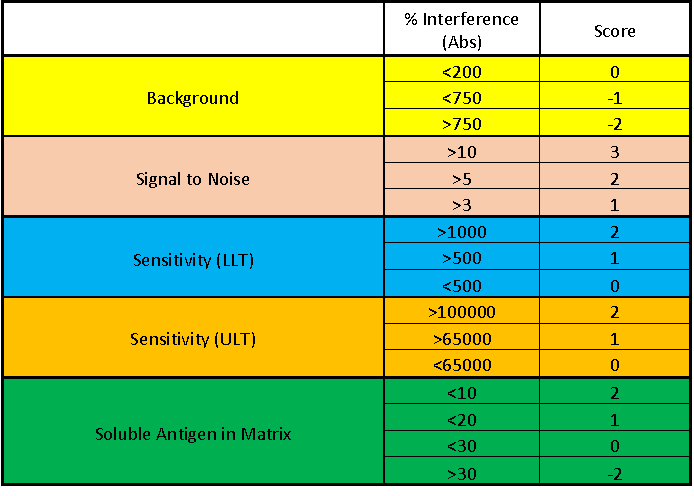
\includegraphics{graphics/ch3/Table_1.pdf}
\end{table} 
 
The example below shows calculation of the Anti-ID 6-Biotin & Anti-ID 6-Tag pairing assay to show how the scores are calculated. The Score fields are empty in the table below and will be filled based on each analytical parameter value.

\begin{table}[ht]
 \centering
 \caption{Excel table displaying example calculations for Anti-ID 6-Biotin + Anti-ID 6-Tag pairing results.}
 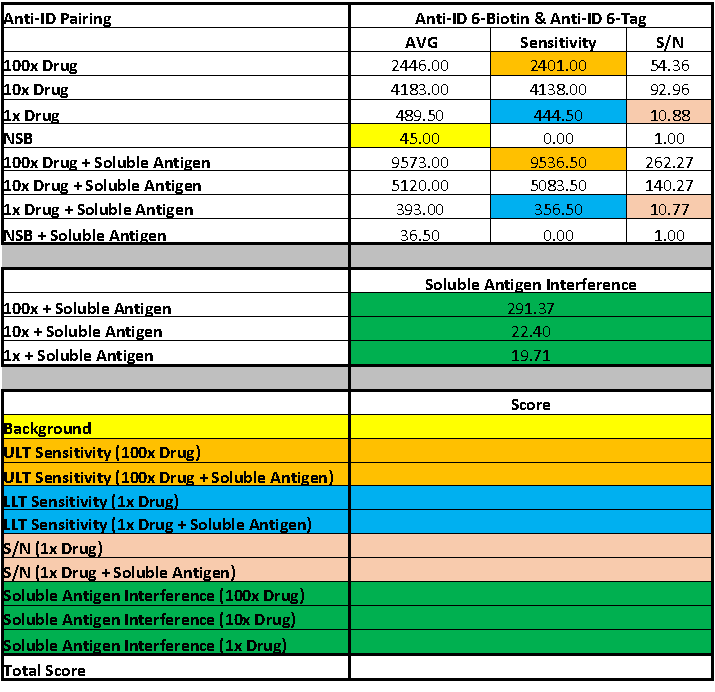
\includegraphics{graphics/ch3/Table_2.pdf}
\end{table} 

We will discuss each of the analytical metric based on the human-defined thresholds to calculate the scores.
\subsection*{Background Calculation:}
The data being scored is highlighted yellow in the table below.  As the background value above is 45, it is$ <$200 and was given a score of “0” shown below.

If the background is below a human-defined absolute value of 200 then it would receive a score of 0; for value between 200 and $<$750, the score is -1 and for value $geq$750, the score of -2.  The negative numbers were chosen for higher backgrounds as high background negatively impacts the assay and this concept was captured by assigning a negative score.  The ranges and score values were decided by human analysts.

For the background score, the higher the background the more negatively this impacted the PK assay and therefore it was assigned a negative score.  It however did not need to be assigned a negative score – it was only given this as it was determined to call out the negative impact on the assay.  The other “positive” scores were given with higher numbers to assign low interference and/or characteristics that would result in a robust sensitive assay.  

\vspace{-1cm}
\begin{table}[ht]
 \centering
 \caption{Excel table displaying background scoring for Anti-ID 6-Biotin + Anti-ID 6-Tag pairing results.}
 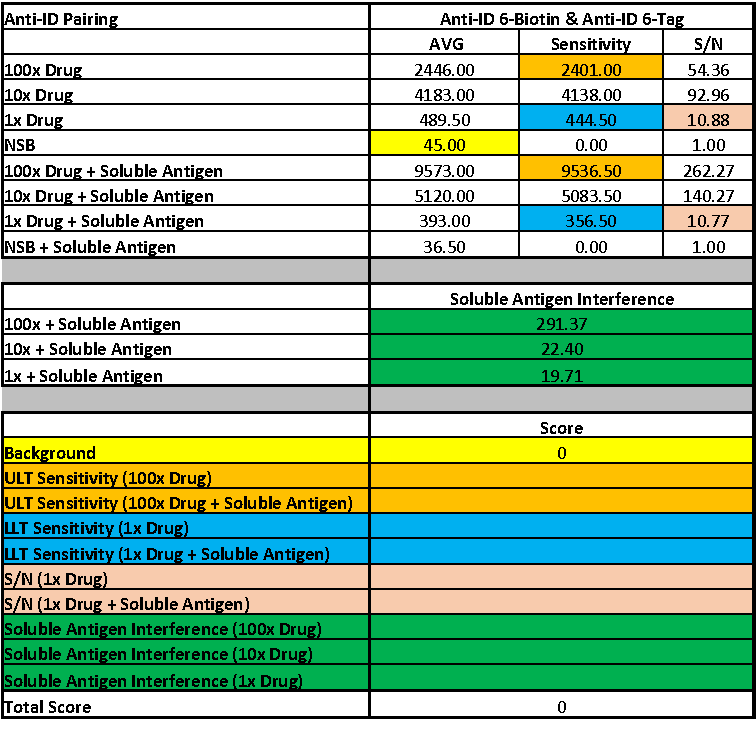
\includegraphics{graphics/ch3/Table_3.pdf}
\end{table} 

\subsection*{Sensitivity (Upper Limit Tested (ULT)) Calculation:}
The data being scored is highlighted orange in the table below.  As the ULT Sensitivity (1x Drug) was 2401.0, it is $<$65000 and was given a score of “0”, for ULT Sensitivity (1x Drug + Soluble antigen) was 9536.5, it is $<$65000 and was also given a score of “0”.

There are two values to be captured for this score +/- soluble antigen.  If the absolute value of the 1x Drug measurement is below 65000 then it would receive a score of 0; between 65000 to $<$100000, it was given a score of 1, and value $\geq$100000, a score of 2 was given.  The positive numbers were chosen for sensitivity (ULT) as the higher the numbers the more robust the assay and this concept captured by assigning a positive score.  The ranges and score values were decided by human analysts.

\begin{table}[ht]
 \centering
 \caption{Excel table displaying sensitivity (ULT) scoring for Anti-ID 6-Biotin + Anti-ID 6-Tag pairing results.}
 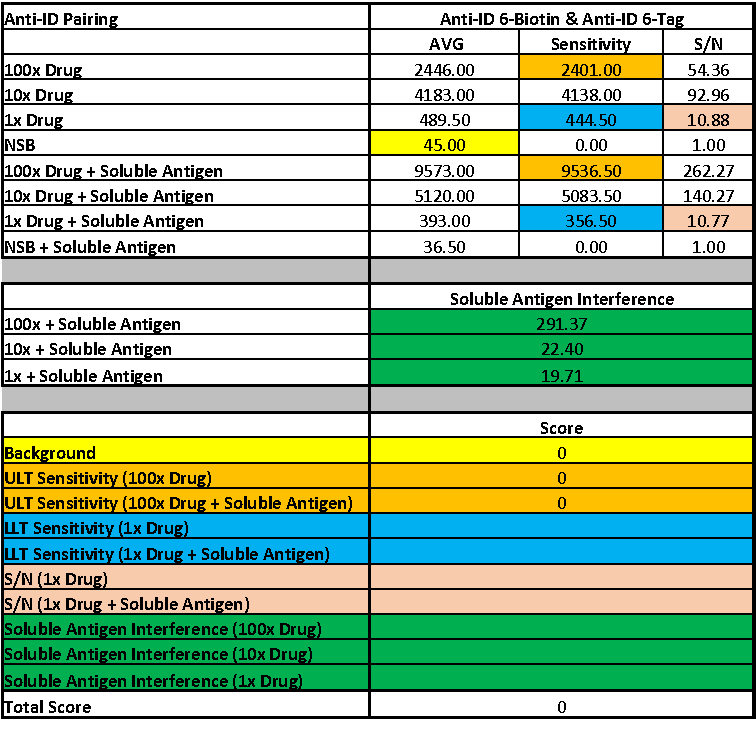
\includegraphics{graphics/ch3/Table_4.pdf}
\end{table} 

\subsection*{Sensitivity (Lower Limit Tested (LLT)) Calculation:}
The data being scored is highlighted blue in the table below.  As the LLT Sensitivity (1x Drug) was 444.5, it is $<$500 and would give a score of “0”, and the LLT Sensitivity (1x Drug + Soluble antigen) was 356.5, it is $<$500 and would also give a score of “0”.

There are two values to be captured for this score +/- soluble antigen.  If the absolute value of the 1x Drug measurement is below 500 then it would receive a score of 0; between 500 to $<$1000, it would receive a score of 1, and $\geq$1000 it would receive a score of 2.  The positive numbers were chosen for sensitivity (LLT) as the higher the numbers the more robust the assay and this concept was captured by assigning a positive score.  The ranges and score values were decided by human analysts.

\begin{table}[H]
 \centering
 \caption{Excel table displaying sensitivity (LLT) scoring for Anti-ID 6-Biotin + Anti-ID 6-Tag pairing results.}
 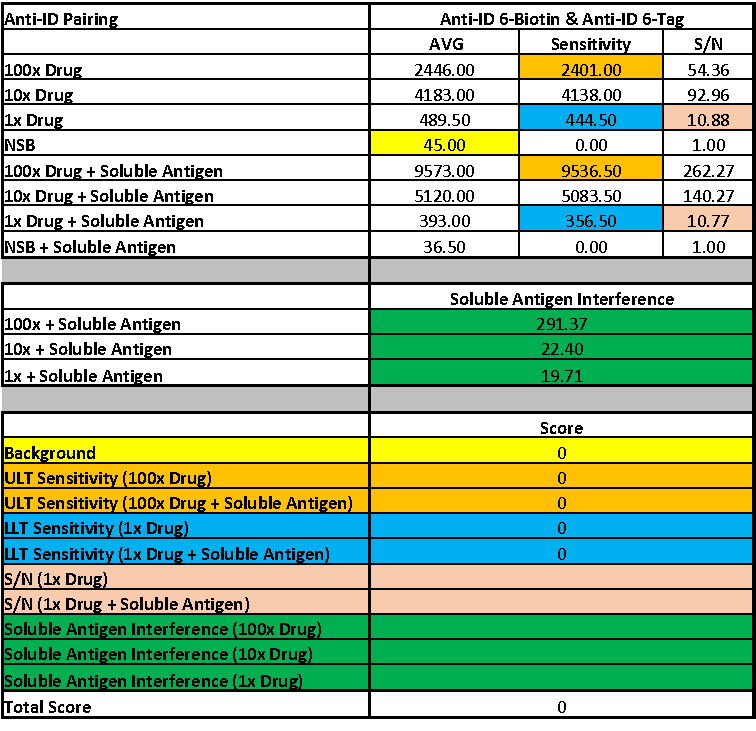
\includegraphics{graphics/ch3/Table_5.pdf}
\end{table} 

\subsection*{Signal to Noise (S/N) Calculation:}
The data being scored is highlighted peach color in the table below.  As the S/N (1x Drug) was 10.88 – it is $>$10 and would give a score of “3”; and the S/N (1x Drug + Soluble antigen) was 10.77 it is $>$10 and would give a score of “3”.

There are two values to be captured for this score +/- soluble antigen. If the absolute value of the 1x Drug measurement/divided by the background is $\leq$3 then it would receive a score of 0; for values $>$3 and $\leq$5, a score of 1; values $>$5 and $\leq$10, it would receive a score of 2 and for values $>$10 then it would receive a score of 3.  The positive numbers were chosen for S/N as the higher the numbers the greater the signal is away from background indicating a strong signal that will yield a robust the assay and this concept was captured by assigning a positive score.  The ranges and score values were decided by human analysts.

\begin{table}[ht]
 \centering
 \caption{Excel table displaying signal to noise scoring for Anti-ID 6-Biotin + Anti-ID 6-Tag pairing results.}
 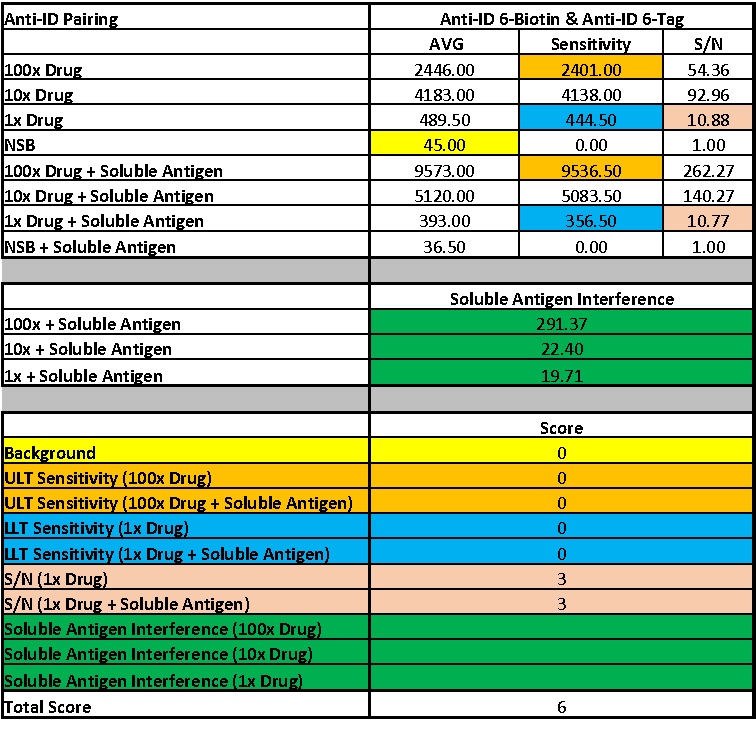
\includegraphics{graphics/ch3/Table_6.pdf}
\end{table} 

\subsection*{Soluble Antigen Interference Calculation:}

\\The data being scored is highlighted green in the table below.  For 100x drug soluble antigen interference value of 291.37, the score is -2, for 10x drug soluble antigen interference value of 22.40, the score is 0, for 1x drug soluble antigen interference value of 19.71, the score is 1.

There are three values to be captured for this score soluble antigen with the 3 different concentrations of drug used.  As an example,
\\
\\
\hspace*{.5in}100x Drug Soluble Antigen Interference = absolute value of
\\
\\
\hspace*{.5in}100*[(100x Drug Average–(100x Drug & Soluble Antigen Average)/(100x Drug Average]
\\
\\
\indent If the absolute value of the soluble antigen interference for X Drug measurement is $<$10 then score is 2; value $\leq$10 and $<$20 will get a score of 1, value $\geq$20 and $<$30 then the score is 0, value $\geq$30 then the score is -2.  The decreasing positive numbers were chosen for soluble antigen interference as the higher the numbers the greater the negative impact on the assay and this concept was captured by assigning decreasing positive scores.  The ranges and score values were decided upon by a collection of analysts.

Adding all the scores lead to the total score of 5, as shown in the table below.

\begin{table}[ht]
 \centering
 \caption{Excel table displaying soluble antigen interference scoring and total scoring for Anti-ID 6-Biotin + Anti-ID 6-Tag pairing results.}
 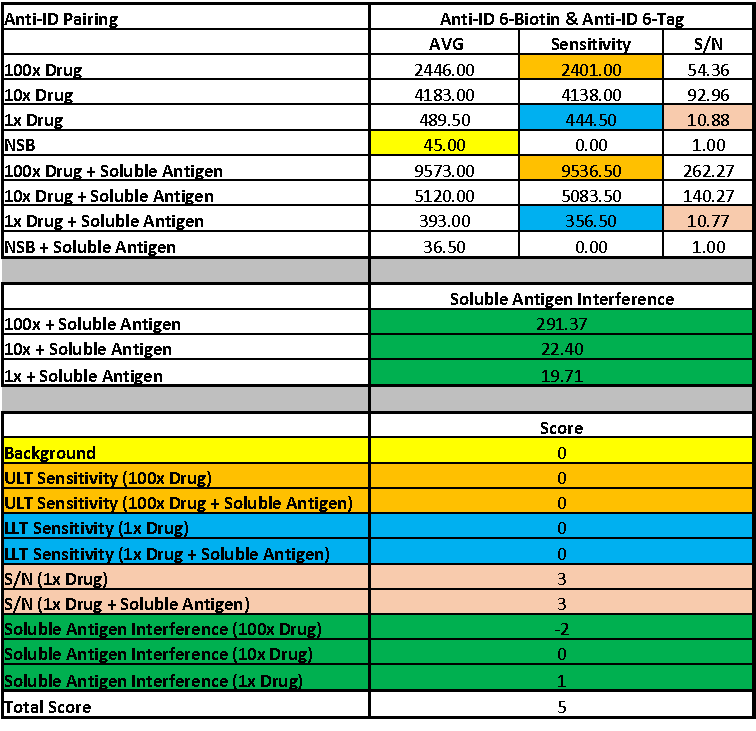
\includegraphics{graphics/ch3/Table_7.pdf}
\end{table} 

\subsection{Scoring Tool}
Initial reagent screening using the ECL assay format focused on interference from the matrix and soluble antigen.  The screening of labeled pairs using different assay formats used a more complex scoring function.  The parameters assessed in this scoring function included background signal, signal to noise, sensitivity, dynamic range, and soluble antigen interference.  These parameters were assessed using 6 different assay formats and at two different anti-ID concentrations. A total score was calculated based on the listed criteria, where analytical parameters were assigned scores.  Parameters with high values, such as background, were given negative scores and positive scores for low values.  The negative numbers were chosen for higher backgrounds as high background negatively impacts the assay and this concept was attempted to be captured by assigning a negative score.  The positive numbers were chosen for sensitivity (ULT, LLT) as the higher the numbers the more robust the assay. The positive numbers were chosen for signal to noise (S/N) as the higher the numbers the greater the signal is away from background indicating a strong signal that will yield a robust assay. The decreasing positive numbers were chosen for soluble antigen interference as the higher the numbers the greater the negative impact on the assay and this concept was attempted to be captured by assigning decreasing positive scores. The ranges and score values were decided by human analysts. However, the use of negative values during scoring was omitted when using data dependent scoring methods.  The initial use of negative values was chosen for ease of interpretability for identifying negative impacts on the assays.

The screening of multiple reagents and assay formats resulted in many assay plates with a large volume of data to be processed to enable the selection of the optimal reagents for the PK assay.  The scoring function was designed to enable the assay developer to weight parameters differently based on assay requirements.  Manually processing this data using a spreadsheet is time-consuming and potentially can introduce errors.  In order to streamline this process, the scoring tool was programmed in Python with a graphical user interface (GUI) to accelerate data processing and provide consistency in using the tool (Supplementary Figures S1-3). 

\begin{figure}[ht]
 \centering
 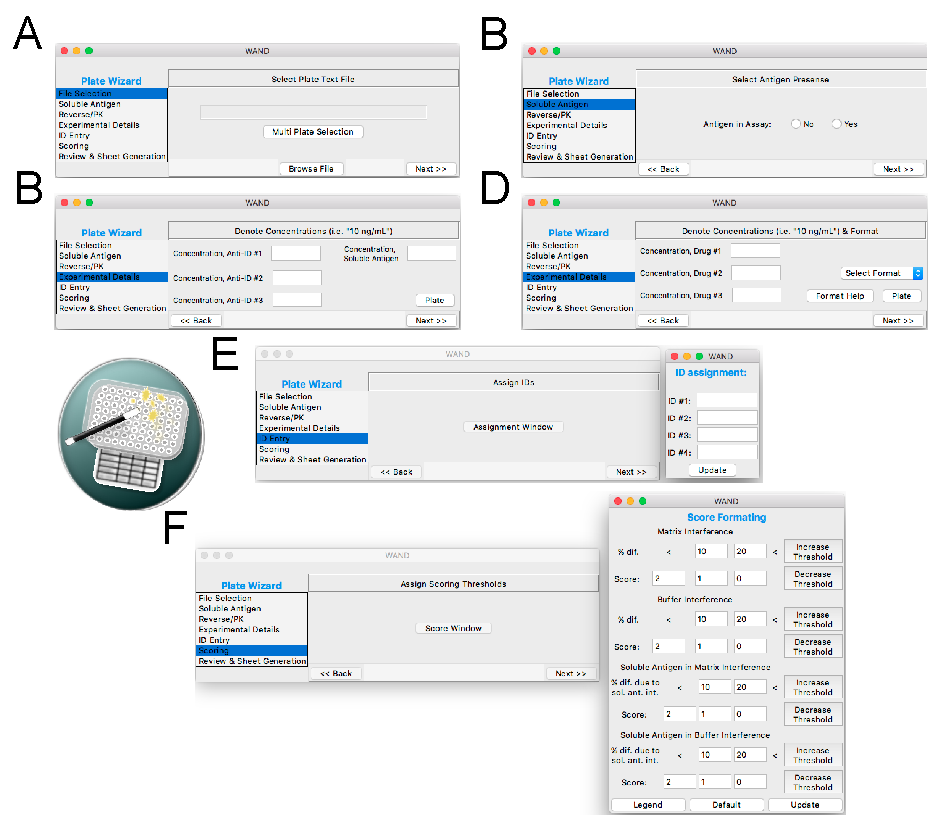
\includegraphics{graphics/ch3/Figure_S1.pdf}
 \caption{WAND: Workflow Automation for Nested Decision is a software tool with graphical user interface to automate experiment set-up and data analysis by incorporating information on several assay formats, detailed error handling for specific formats and automated data analysis to minimize human error. The user specifies different assay parameters, conditions, and scoring weights, generating comprehensive reports as excel sheets for further analysis. (A) The file selection panel allows WAND to access and process plate reader files. (B) The antigen selection and screening type panels allow the user to specify the appropriate experimental descriptors for a given plate reader file.  (C&D) The experimental details, and subsequent panels, are displayed such that prior specifications dictate the inputs available that ensure proper descriptor entry.  (E) ID entry is performed in a separate window which allows users to input the appropriate name of reagents.  (F) Dynamic scoring entry allows for users to modify the interpretation of plate reader files such that desired analytical values are given higher pertinence post analysis.}
 \end{figure}
 
\begin{figure}[ht]
 \centering
 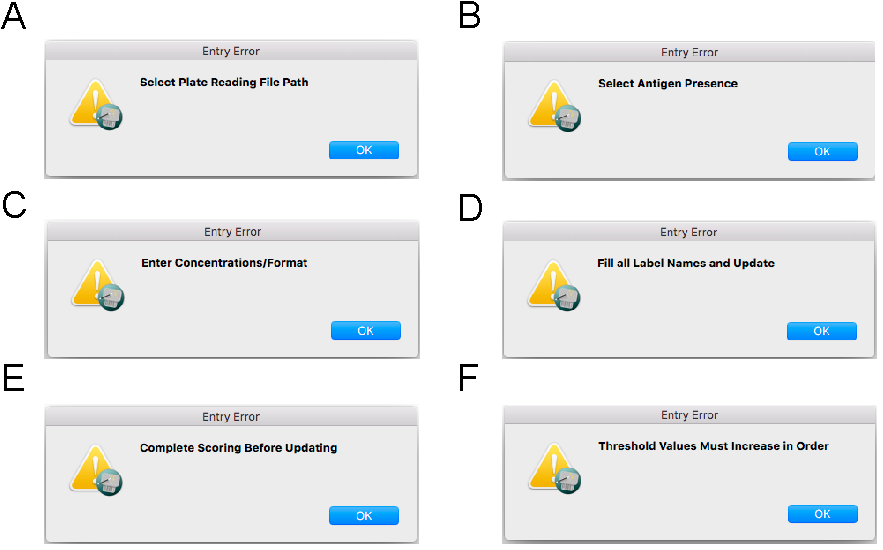
\includegraphics{graphics/ch3/Figure_S2.pdf}
 \caption{Showing error handling in WAND to ensure all information needed to produce a complete data analysis report is provided by the user.  Error statements are prompted by premature toggling of the next interface display when: (A) no plate reader file is uploaded, (B) no selection of antigen presence in a plate assay and similarly if a generic or PK screen was run, (C) descriptive experimental details such as drug concentration or PK format are omitted when required, (D) absent reagent label descriptors, (E) absent values when entry boxes are present in the scoring window, and (F) the entry of non-increasing numeric values for the thresholds of a given analytical scoring metric.}
 \end{figure}

\begin{figure}[ht]
 \centering
 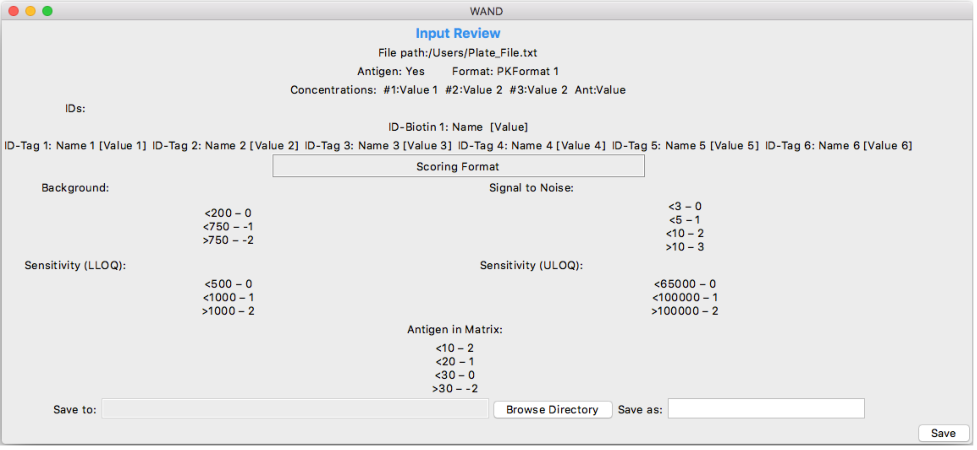
\includegraphics{graphics/ch3/Figure_S3.pdf}
 \caption{Example of a review screen prompted by WAND prior to generation of an analysis report sheet.  All user inputs are captured and displayed to allow users to ensure the correct information has been provided prior to designating the location and name of the report to be generated.}
 \end{figure}

\subsection{Data Dependent Scoring}
The scoring functions used for ranking ECL-based anti-ID screening and PK assay formats along with anti-ID pairing screens were done in a data-dependent manner using Gaussian mixture models (GMMs).  Instead of using predetermined human-identified thresholds, GMMs fits a number (\emph{K}) of weighted Gaussian distributions called mixture components to the data.  By fitting the values of assay conditions evaluated by scoring functions, the GMM pipeline clusters and classifies data-points (\emph{x}) into a class (\emph{c}) corresponding to a mixture component.  The data-points are classified by treating their maximal probability under the weighted Gaussian distributions as their ‘class label’ (y\textsubscript{\emph{l}}) as given in eq. 3.1. 

\begin{equation}
y_l:=\argmax_ip(c_i\vert x),\,c_i\in \{0…K\}
\end{equation}
The GMM pipeline was developed such that the number of Gaussian distributions was selected by fitting GMMs with the number of Gaussians ranging from four to ten and selecting the model with the lowest resulting Akaike information criterion.  Absolute values of data-points were first min-max normalized prior to evaluation using the GMM based data dependent scoring pipeline.  The GMM based data dependent scoring pipeline was implemented by fitting GMMs to both individual parameters and the full set of parameters simultaneously.  For cases where lower values are desired for parameters used to evaluate PK assays, the absolute values of data-points were made negative prior to normalization when evaluating all parameters simultaneously.  Scores for ranking were assigned to clustered data points by assigning increasing integer values, starting from zero.  The Euclidean norm was used to measure cluster means from a vector comprised of elements all equal to zero or all equal to one for ECL-based anti-ID screening and PK assays respectively, when evaluating all parameters simultaneously.  Clusters were then assigned their rank order, starting from zero, in order of decreeing Euclidean distance measures.  When evaluating individual parameters, cluster means would have their measures calculated from either zero or one vectors depending on if lower or greater parameter values were respectively desired.  

Covariance regularization of the mixture models was applied when evaluating individual parameters such that elements of the covariance matrix off the diagonal were weighted to zero.  Otherwise, the covariance matrixes were unregulated when evaluating all parameters simultaneously.  GMMs were implemented using the Scikit-learn (Version 1.0.2) Python library with all parameters, excluding the number of components and covariance regularization types, left as default values.  Results were visualized using Uniform Manifold Approximation and Projection (UMAP) for cases where all parameters were evaluated.  UMAPs were generated using the umap-learn (Version 0.5.3) Python package.  For the generic indirect ELISA screening studies UMAP parameters were defined as: \emph{‘n{\_}components’} set to 2 , \emph{‘n{\_}neighbors’} set to 15, and \emph{‘min{\_}dist’} set to 0.25.  For PK studies UMAP parameters were defined as: \emph{‘n{\_}components’} set to 2 , \emph{‘n{\_}neighbors’} set to 50, and \emph{‘min{\_}dist’} set to 0.25.  Both uses of UMAP used a Euclidean metric. Cumulative scores were summed from min-max normalized GMM produced scorings, with normalization being applied to the scores of each experimental trial with varied concentrations of antigen or anti-IDs.  All code for GMM and UMAP studies was run in Python 3.7.11, and is available with plots on Github at \emph{https://github.com/chopralab/Bioanalytical\textunderscore Assay\textunderscore Manuscript\textunderscore Repo/tree/main/GMMs}.


\section{Results}
\subsection{Generation of Anti-IDs and Initial Selection}
Anti-idiotypic antibodies were generated using the Fab fragment of a proprietary therapeutic antibody.  Ten mice from 2 different strains were immunized 3 times and serum was collected.  The antibody titer for each mouse was determined using an ELISA assay with the therapeutic Fab region used as the capture and a goat anti-mouse IgG-HRP was used for detection.  Two mice with the highest titers were euthanized for generation of hybridomas with their lymphocytes from spleens and the myeloma fusion partner.  This resulted in 18 clones with specific binding to the mAb from the primary screening of the anti-ID antibodies (Table S1).  This panel of anti-IDs were high affinity antibodies with most KD values less than 100 nM (Table S2).    The epitope binning data indicated that the 18 anti-IDs all bind to closely related epitopes and are in the same epitope bin with the response percentages $<$10\% (Table S3).  The resultant 18 clones were chosen for further screening to determine the optimal anti-IDs to bind to the mAb in the presence of soluble antigen.

\begin{figure}[ht]
 \centering
 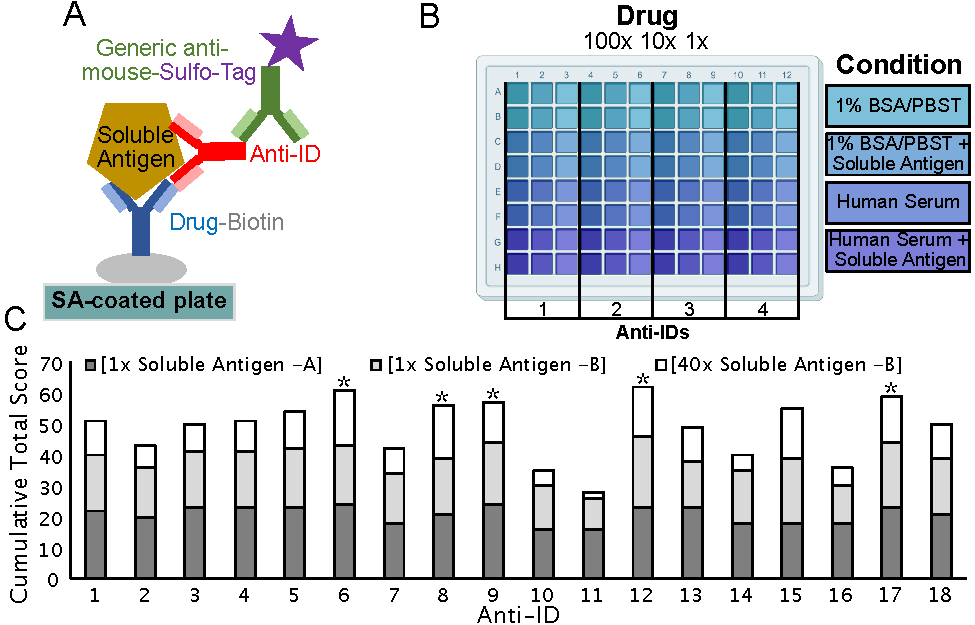
\includegraphics{graphics/ch3/Figure_1.pdf}
 \caption{Generic indirect ELISA initial screen of anti-IDs in the presence of matrix and soluble antigen. A) Schematic diagram of generic indirect ELISA with soluble antigen. B) Representative plate layout for generic ELISA screen.  Four anti-IDs across 2 orders of magnitude of concentration were screened per plate +/- human serum and/or soluble antigen.  C) Scoring matrix used to rank order anti-IDs based upon impact of matrix and soluble antigen interference.  D) Cumulative total scores for anti-IDs in the presence of 1x or 40x soluble antigen.  (*) indicate anti-IDs selected for labeling.}
 \end{figure}

Traditional methods for functional screening of anti-IDs involved labeling each anti-ID for capture and detection.  For 18 different anti-IDs this is a laborious process resulting in a large number of labeled reagent enumeration to screen every potential pairing.  To this end, 324 different combinations would need to be tested per assay format, at a single concentration, if a traditional approach was used.  Therefore, an indirect format (Figure 1A,B) was used to perform an initial screen of anti-IDs to examine the effects of matrix (pooled human serum) and soluble antigen interference on the ability of the anti-IDs to bind to the therapeutic antibody.  A standardized plate map was also selected to allow for development of automation procedure and for the future use of this workflow in screening anti-IDs in other projects.  In addition, a scoring system was established to rank order the anti-IDs based on the effect of 1) soluble antigen interference in buffer, 2) matrix interference (blank serum), 3) soluble antigen in matrix versus buffer, and 4) soluble antigen in matrix versus blank matrix (Figure 1C).  This was performed at three levels of each anti-ID (1x, 10x, 100x) in the presence of soluble antigen that was calculated to be at least 10x greater than the lowest expected levels of soluble antigen in patients.  Additionally, this format was tested in the presence of 40x of the soluble antigen for super saturating conditions of soluble antigen.  The composite scores from each experiment were tabulated and are shown in Figure 1D. Complete data and scoring are in Supplementary Tables 4-6.  The top five anti-IDs (6, 8, 9, 12, 17) with the highest composite score and the least interference from matrix and/or soluble antigen were then selected for progression to a more rigorous labeled-anti-ID sandwich assay format. 

\begin{figure}[ht]
 \centering
 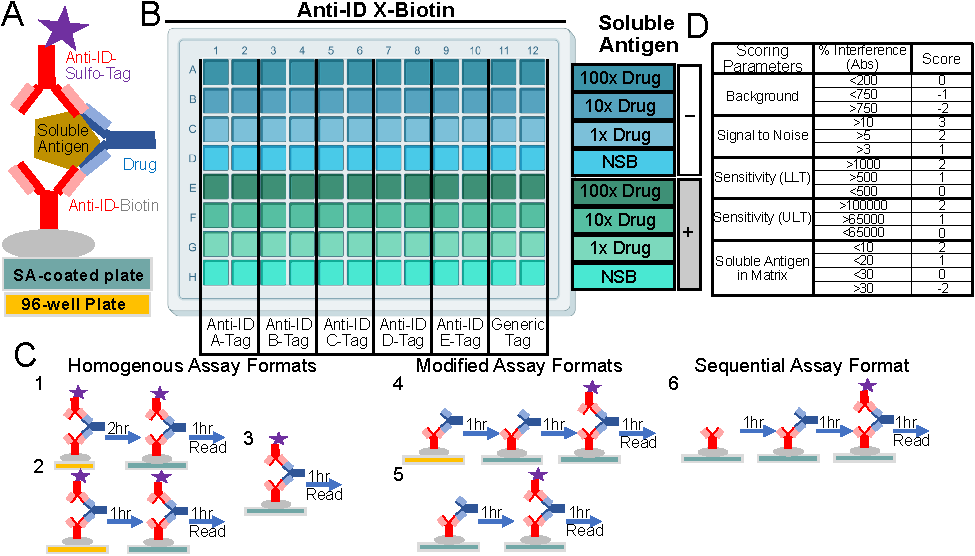
\includegraphics{graphics/ch3/Figure_2.pdf}
 \caption{Labeled anti-ID pairings and sandwich PK assay format screening approach.  A) Schematic diagram for sandwich anti-ID ELISA screening.  B) Representative plate map for labeled anti-ID screen.  Six Sulfo-TAG-anti-IDs were used per plate with a single biotinylated-anti-ID to measure the concentration of therapeutic $\geq$2 orders of magnitude +/- soluble antigen.  The non-specific binding (NSB) +/- soluble antigen was also measured.  C) PK assay formats screened.  Six PK assay formats were screened: three homogenous formats, two modified assay formats, and one sequential assay format. D) Scoring matrix for rank ordering of anti-ID pairings with analytical parameters using absolute interference.}
 \end{figure}


The five selected anti-IDs (6, 8, 9, 12, 17) were labeled with biotin and Sulfo-tag and used as both capture and detection reagent in the next screening step (Figure 2A).  These labeled reagents were used to determine the best pairing for a PK assay resulting in 25 different possible pairing combinations.  Additionally, a generic mouse anti-human IgG4 was used as a detection reaction in combination with the 5 different capture reagents for a total of 30 pairing combinations.  A standardized plate map was again utilized to enable use of automated liquid handlers and the automated scoring tool (Figure 2B).  The anti-ID screening for PK assay development has historically been done on a ‘fit-for-purpose approach’ wherein the anti-IDs are typically screened in a pre-defined assay format at a single concentration [17]. Once the reagent pair is identified by the pre-defined assay format, other assay formats are tested to further optimize the performance of the assay. However, a limitation exists, in that the best reagent pair selected by the pre-defined assay format is not necessarily the best pair of reagents for other assay conditions. Given the interdependence of reagents combination, concentration and assay formats, a more comprehensive approach was developed with 30 anti-ID pairings that were tested with two different concentrations (0.25 µg/mL and 1.0 µg/mL) in six different PK assay formats (Figure 2C).  These pairings of anti-IDs were screened across $\geq$2 orders of magnitude of the mAb +/- soluble antigen.  

\begin{figure}[H]
 \centering
 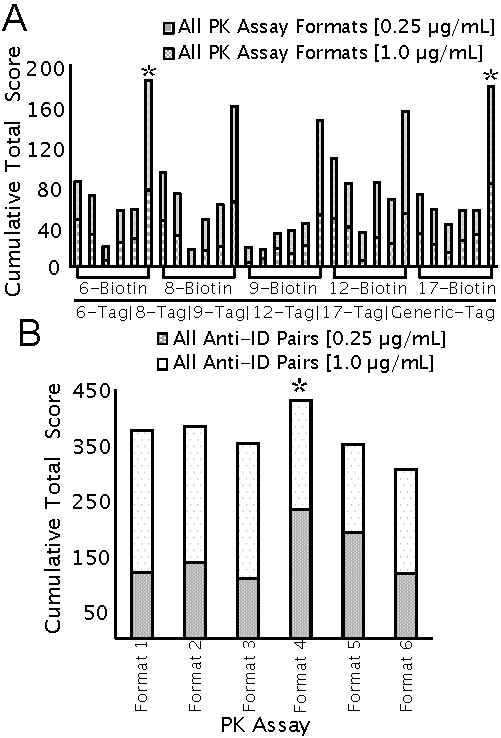
\includegraphics{graphics/ch3/Figure_3.pdf}
 \caption{Labeled anti-ID pairings and sandwich PK assay format screening results. A) Cumulative total score of two concentrations of anti-ID pairings across all PK assay formats.  Scores were established for each anti-ID pairing/PK assay format per concentration.  The scores of all six PK assay formats per anti-ID pairing were tabulated.  The top two pairings across all PK assay formats are indicated by (*).  B) Cumulative total score of PK assay formats across all anti-ID pairings.  The scores of all anti-ID pairings per PK assay format were tabulated.  The top PK assay format is indicated by (*).}
 \end{figure}

A second scoring system was developed to determine both the best pairing and optimal PK assay format.  The parameters measured and scored include: 1) background signal, 2) signal to noise, 3) sensitivity LLT (lower therapeutic concentration counts), 4) sensitivity ULT (upper therapeutic concentration counts), and 5) soluble antigen in matrix (Figure 2D).  Parameters 1 to 4 were assessed in the presence and absence of soluble antigen.  The cumulative scores for both concentrations of anti-IDs across all PK assay formats tested are displayed in Figure 3A.  The generic-tag detection reagent was the best detection reagent regardless of the anti-ID capture or concentration as the top five scores all had the generic-tag for detection (Figure 3A; Supplementary Table 4, 5).  Further, the anti-ID #6 had the greatest cumulative score across all PK assay formats tested with anti-ID 17 selected as the back-up with the second top score.  The pairing of anti-ID #6-Biotin/Generic-Tag had the maximal score, 20, in both concentrations tested, while the pairing of anti-ID #17-Biotin/Generic-Tag had the maximal score at 0.25 g/mL and a score of 18 at 1.0 µg/mL due to soluble antigen interference at 10x drug (Supplementary Table 4, 5).  These anti-IDs were both selected to generate large-scale recombinant proteins for future use in the development and validation of the clinical PK assay.  Assay format 4 had the greatest cumulative score for all anti-IDs across both concentrations tested (Figure 3B; Supplementary Table 4, 5) and was selected as the optimal PK assay format.  

\begin{figure}[H]
 \centering
 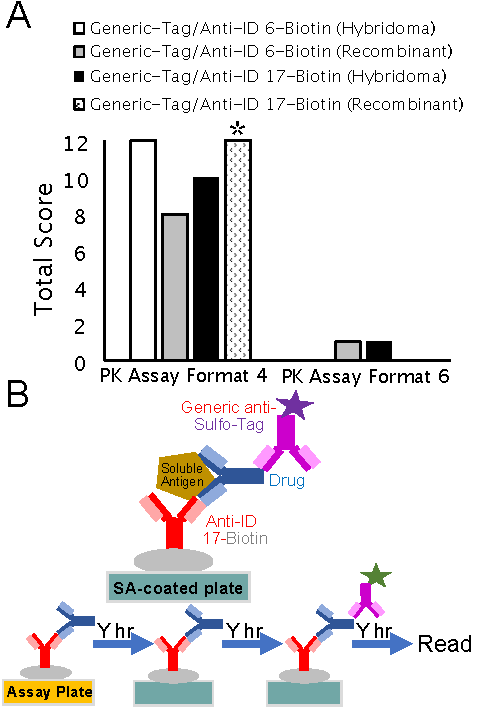
\includegraphics{graphics/ch3/Figure_4.pdf}
 \caption{Final anti-ID pairing and PK assay format selection.  A) Recombinant anti-ID pairings were compared to original hybridoma pairings in two different PK assay formats.  Scores were calculated based upon previous criteria listed in Figure 2D.  The total score of for each pairing/format was tabulated.  The final recombinant pairing selected is indicated by (*).  B) Schematic of final anti-ID pairing and PK assay format that were selected.}
 \end{figure}


Large-scale recombinant proteins for anti-ID #6 and #17 were generated and these pairings were compared with the original hybridoma reagent pairings in PK assay formats 4 and 6 to confirm the selection of optimal PK assay format and anti-ID pairing (Figure 4A; Supplementary Table 6).  PK assay format 4 yielded higher scores relative to assay format 6 indicating this to be the optimal PK assay format for these anti-ID pairings.  There was a decrease in sensitivity and signal to noise scores that resulted in a decreased total score for the anti-ID 6-Biotin/Generic-Tag recombinant pairing compared to the hybridoma pairing.  However, there was an increase in signal to noise score in the anti-ID #17-Biotin/Generic-Tag recombinant compared to the hybridoma (Figure 4A).  This increased total score resulted in the selection of anti-ID #17-Biotin/Generic-SulfoTag recombinant pairing in PK assay format 4 as the final PK assay (Figure 4B). 
\subsection{Scoring Tool and Graphical User Interface}
Data handling and analysis is a tedious task during an execution of automated assays formats. The scoring metrics for generic and PK assay formats was compiled with Workflow Automation for Nested Decisions (WAND) to facilitate the rapid analysis of data from several experiments to make decisions (Figure S1). Further, detailed error handling for specific formats was implemented to minimize human error during experimental set-up, parameter selection and interpretation (Figure S2). The user specifies different assay parameters, conditions and scoring weights in a stepwise manner to generate comprehensive reports (Figure S3) for further analysis. The modularity of the GUI makes it easy to go beyond the six specified PK assay formats and makes WAND an ideal choice to develop robust automated PK assay workflows.

\subsection{Gaussian Mixture Model Based Scoring}

\begin{figure}[H]
 \centering
 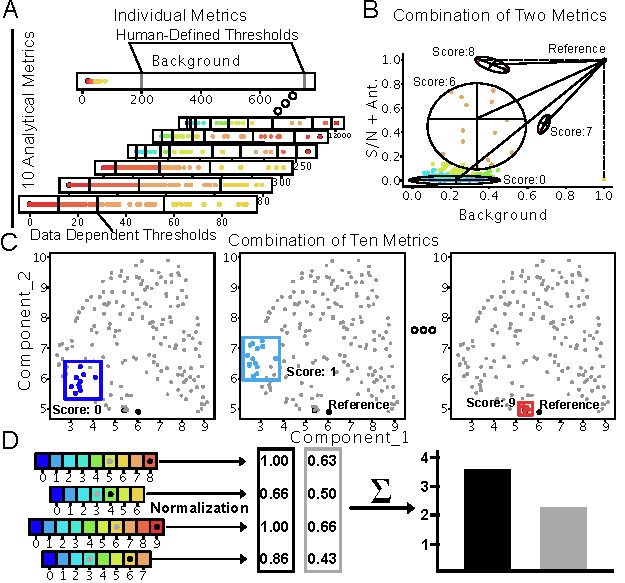
\includegraphics{graphics/ch3/Figure_5.pdf}
 \caption{Schematic of data dependent scoring.  Showing representative data for PK assays (1µg/mL) A) Data from individual metrics were clustered using GMMs, resulting in new thresholds (black) which further differentiate interference distributions compared to human-defined thresholds (grey).  B) Extension of the GMM scoring approach where data from two metrics are clustered simultaneously.  Clusters are ranked by their mean distance from a point defined by the best values of each individual analytical parameter.  C) Extension of the GMM scoring approach by incorporating all 10 analytical parameter associated with PK assays.  Clustering is done in 10-Dimensional space, and displayed as a 2-Dimensional UMAP, with selected clusters displaying their respective coloring and scores. Reference indicates the origin or the best possible score in higher dimensions which is used for scoring clusters.  D). Schematic displaying the scoring to assay ranking pipeline, where scores derived from GMM clusters are normalized and followed by summation.}
 \end{figure}

The scoring systems previously described were replicated in a data dependent manner by use of GMMs.  Evaluation of parameters was done both by fitting GMMs to each parameter individually and by fitting a single GMM using data-points representing vectors comprised from normalized values from each parameter (Figure 5).  The data dependent scoring approach replicated selections derived from cumulative scores with high overlap.  Using the approach of fitting GMMs to each parameter individually, two of the selected anti-IDs from ECL-based screening again yielded cumulative scores within the top five (Figure S4-7) and fully replicated the selections for anti-ID pairings and PK assay format (Figure S8-9).  When using a single GMM to evaluate all parameters simultaneously, the perfect overlap in PK assay results was maintained, while identifying an additional anti-ID that was selected using human-defined thresholds for evaluating ECL-based screenings.  

\section{Discussion}
Ligand binding assays (LBAs) have been widely used to quantify the amount of biological drug molecules in pharmacokinetic studies.  The reagent screening and assay development of LBAs to measure PK have traditionally used a semi-empirical approach.  However, the increased usage and development of therapeutic antibodies presents an opportunity to develop and use a systemic approach to increase efficiency, quality, and robustness of the LBA PK assay.  For some therapeutic antibodies, the presence of a circulating soluble target could interfere with the PK assay performance and requires consideration to ensure total drug levels can be measured, that includes both free and target-bound drug.  Identification of reagents with a high binding affinity specifically for the mAb regardless of presence of soluble target and a low matrix interference are key qualities for the optimal reagent.  However, the most robust PK assay cannot be developed with such reagents if the optimal PK format for these reagents has also not been selected.  Therefore, screening and selection of critical reagents concurrently with the determination of the most robust assay format are key components in developing a robust PK assay capable of measuring free and bound mAb levels in serum.    
  
Anti-IDs were generated through creation of hybridomas from immunizations of mice with the Fab fragment of the therapeutic mAb.  Multiple characteristics of the anti-IDs including the binding kinetics, affinities for the mAb and epitope binning were determined to attempt to triage the number of Anti-IDs to be screened.  The results of the binding kinetics and affinities showed similar characteristics for all anti-IDs generated in the present study, and all of these anti-IDs were found to be in the same epitope bin.   These results required all 18 anti-IDs to move forward to be screened to determine the optimal reagents for the PK assay.  However, these results did not account for the effects of matrix and/or soluble antigen interference on the ability of the anti-IDs to bind to the mAb.  In addition, hybridomas often lead to a large number of clones and it is inefficient and costly to label and screen all clones.  Therefore, a two-step strategy was developed to identify optimal reagents and assay format to differentiate and select anti-IDs using an ECL screening assay and then a labeled anti-ID sandwich ECL screening assay with a GUI to do multiple scoring parameters analysis.  This strategy was successful in identifying the most robust PK assay format with the optimal reagents for a mAb.    

The first phase of the strategy involved using a generic screen of the anti-IDs with a biotinylated mAb as a capture and an anti-mouse IgG-HRP as a detector (Figure 1A-B).  This initial screen allowed for determination of both the effect of matrix and soluble target interference on the ability of the anti-IDs to bind to the mAb.  A scoring system was used to rank-order the anti-IDs that assigned a numerical value to four different parameters based upon the effects of matrix and soluble antigen interference (Figure 1C, D; Supplementary Tables 1,2,3).  The use of this scoring system allowed for identification of anti-IDs that had the lowest cross-reactivity to human serum and interference from soluble antigen.  Identifying the anti-IDs with the top scores decreased the number of pairs of anti-IDs to use in a labeled screen and allowed for a more targeted investigation into the optimal anti-IDs and PK assay format.  The top five performing anti-ID’s based on their scores and a generic detection reagent were chosen to move to the second stage of screening.

Following the selection of anti-IDs for the second phase, the anti-IDs were both biotinylated and Sulfo-tagged to be used in a pairwise sandwich ECL assay with the therapeutic mAb.  This screening was done at three concentrations of mAb across at least 2 orders of magnitude in the presence and absence of the soluble target.  In addition, six different PK assay formats and two concentrations of anti-IDs were used to simultaneously identify the most robust PK assay format and optimal reagent combination and concentration.  A second scoring system measuring ten different parameters was used to determine the optimal anti-ID pairing and PK assay format (Figure 2C, D, Figure 3A, B; Supplementary Tables 4,5).  The ten parameters include, 1) background signal, 2) and 3) signal to noise with and without soluble ligand, 4) and 5) upper level of quantitation with and without soluble ligand, 6) and 7) lower level of quantitation with and without soluble ligand, and 8), 9) and 10) soluble ligand interference at three different drug levels. This multifactorial scoring system identified the top two performing pairs of ant-IDs in the PK assay format that would yield the most robust PK assay (Figure 3A and 3B).  These results were further confirmed by the results the recombinant anti-ID pairings (Figure 4A and 4B).  To enable this complex approach, all assay steps were automated on a liquid handling system to ensure consistency of the method given the range of pipetting steps required on each sample plate and the number of total plates created.

Anti-IDs clones #6 and #17 as capture and the generic a Sulfo-TAG-mouse anti-human IgG4 using assay format 4 were provided used to perform full assay optimization.  Recombinant versions of these clones were generated for further testing.  The modified assay format (Format 4, Figure 2C) of preincubation of the sample with the biotinylated capture reagent prior to transferring to the streptavidin MSD assay is not a typical format.  This approach was repeated and compared to the more traditional sequential format (Format 6, Figure 2C).   Soluble ligand that potentially could interfere with assay performance was used to test for interference.  Both the reagent from the hybridoma and the scaled up recombinant anti-ID confirmed that using the modified Format 4 provided better overall assay performance.  The recombinant version of the backup clone (Clone #17) provided better overall performance when compared to the recombinant version of Clone #6.  This reagent pair and assay format was taken into full assay validation to support the clinical development program.
The two-step screening strategy outlined herein provides a framework for efficient screening of anti-IDs and identification of the most robust PK assay format.  Using fixed plate maps in this approach allowed for the use of automation and development of the WAND scoring tool (Figure S1-3), which together provide an additional layer of uniformity and eliminates potential operational variability.  The scoring system that was developed was also designed to allow for changing of the weighting of the individual scores as needed.  This could occur if there is additional knowledge on the mAb or program indicating that a parameter has potentially more impact on the necessary PK results.  The scoring system for each parameter additionally can be expanded if there is a need to further differentiate the anti-IDs.  Combining fixed plate formats with easily interchangeable elements in this strategy allows for use of these tools in future anti-ID screenings and PK assay development.

\begin{figure}[H]
 \centering
 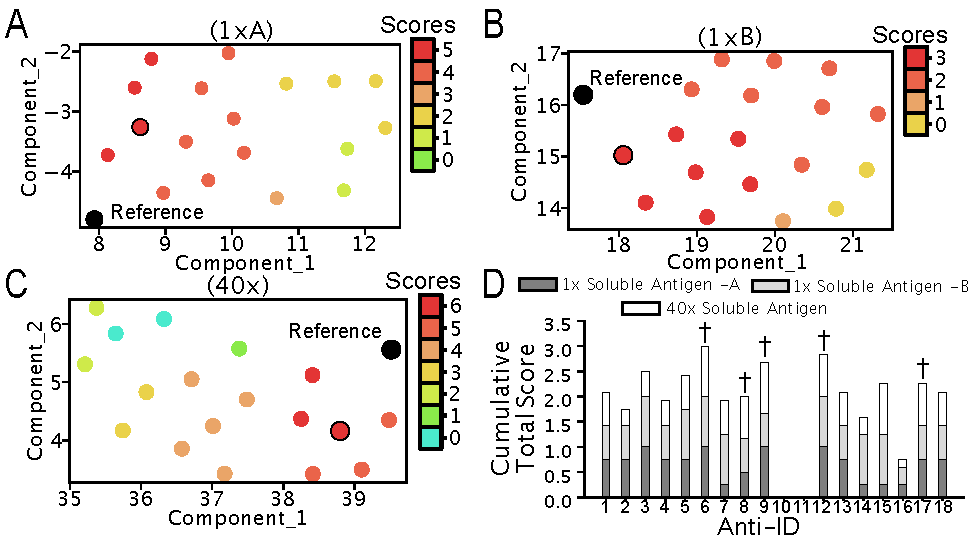
\includegraphics{graphics/ch3/Figure_6.pdf}
 \caption{GMM clustering and by combining all analytical parameters of generic indirect ELISA initial screen of anti-IDs in the presence of matrix and soluble antigens and cumulative scorings. UMAP embeddings of GMM clustered data-points comprised of the four analytical parameters at three concentrations of anti-IDs (total 12-Dimensions). Reference indicates the origin in 12-Dimensions with the best possible score.  A) Clustering of anti-IDs with 1x soluble antigen -A.  B) Clustering of anti-IDs with 1x soluble antigen -B.  C) Clustering of anti-IDs with 40x soluble antigen.  D) Cumulative total scores for anti-IDs in the presence of 1x or 40x soluble antigen.  (†) indicates anti-IDs selected for labeling by using human-defined thresholds for scoring.}
 \end{figure}

\begin{figure}[H]
 \centering
 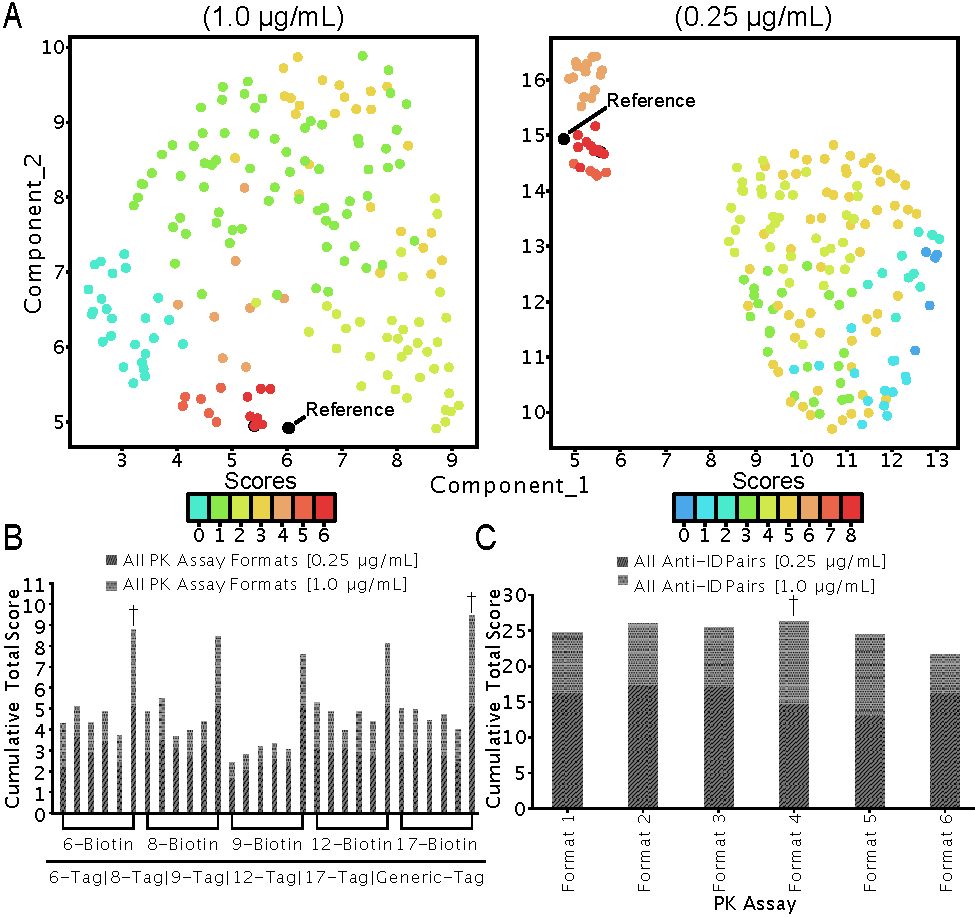
\includegraphics{graphics/ch3/Figure_7.pdf}
 \caption{GMM clustering and cumulative scoring of anti-ID pairings across several sandwich PK assay formats by combining all analytical parameters. UMAP embeddings of GMM clustered data-points comprised of the five analytical parameters, with ULT and LLT and signal to noise used in the presence and in absence of soluble antigen and soluble antigen interference at three separate drug concentrations (total 10-Dimensions). A) GMM clustering on a combination of all ten metrics at a concentration of 1 µg/mL and at a concentration of 0.25 µg/mL. Reference indicates the origin in 10-Dimensions with the best possible score. B) Cumulative total scores of anti-ID pairings across all formats.  Anti-ID pairings are plotted such that a biotinylated reagent and its six Sulfo-tag pairings are plotted sequentially, with the sequence of Sulfo-tag reagents repeating (see Figure 3A). C)  Cumulative total scores of PK assay formats across all anti-ID pairings.  (†) indicate the top anti-ID pairings and PK assay formats selected using human-defined thresholds for scoring.}
 \end{figure}

The data dependent scoring using GMMs broadly captured the robustness of the top assay conditions selected using human based thresholds for the analytical parameters used for scoring (Figure 6, 7, S7, S9).  While both evaluating parameters individually or in unison with GMMs fully replicated the selection of anti-ID pairings and formats for PK assays (Figure 9B-C, S9), the visualized results of individual parameter evaluation by GMMs show further differentiation of assay conditions compared to human based thresholds (Figure S5-7, S9).  Notable examples of the robustness of the GMM based scoring approach are displayed when fitting individual GMMs to PK assay screening results (Figure S9), such as where exceptional results regarding ULT sensitivity are furtherly reinforced.  The use of an automated data driven method for scoring assays removes a large component of human bias and eliminates errors introduced when scoring manually.  Future work on the scoring system aims to leverage automated data science driven approaches towards developing active learning methods. Such predictive machine learning algorithms will facilitate the generation of screening conditions to further expedite the selection and discovery of the optimal anti-IDs with minimum number of experiments.  We envision that developing automated frameworks will facilitate the development of ligand-based assays to enhance the discovery process without human bias.

\section{Conclusion}
An automated bioanalytical workflow for screening anti-IDs to determine the optimal pairing of reagents and PK assay format has been developed.  Fixed plate maps were employed for use with automation with an optimal and flexible scoring system to create a strategy that resulted in significant savings of time (days versus weeks) and resources to develop a novel and robust PK assay for a mAb.  With the increase of therapeutic antibodies as novel drugs, an automated assay and data dependent analysis strategy that allows for rapid identification of critical reagents and development of PK assay will become increasingly more important for supporting human clinical trials.  The proposed automated workflow and tools were successfully used to develop a bioanalytical assay for supporting a clinical program is being implemented for the continued support of antibody drugs. Automation based on learning from data will result in faster discovery and removal of human bias from data interpretation and candidate selection to develop new antibody drugs.

\section{Future Directions}

\newcolumntype{?}[1]{!{\vrule width #1}}

\begin{table}[H]
\begin{center}
\caption{Long Title}
\label{tab:test}
\begin{tabular}{?{1.5pt}m{.78in}?{1.5pt}m{1.25in}| m{1.21in}| m{1.21in}|}
\Xhline{1.5pt}  
&\multicolumn{3}{?{1.5pt}l|}{\cellcolor{grey!25}\textbf{Screening (OD450 nm)}} \\
\Xhline{1.5pt}  
\cellcolor{grey!25}\textbf{Clone No.}&\cellcolor{grey!25}\textbf{Therapeutic mAb} &\cellcolor{grey!25}\textbf{Human IgG#1} & \cellcolor{grey!25}\textbf{Human IgG#2}\\
\Xhline{1.5pt}  
1	&2.98&	0.31	&0.32\\
\hline
2	&3.24	&0.21	&0.26\\
\hline
3	&3.26	&0.24	&0.28\\
\hline
4&	3.19	&0.17	&0.23\\
\hline
5&	3.45	&0.21	&0.26\\
\hline
6&	3.43	&0.26	&0.21\\
\hline
7&	3.31	&0.26	&0.29\\
\hline
8&	3.31	&0.16	&0.2\\
\hline
9&	3.31	&0.26	&0.32\\
\hline
10&	3.22	&0.16	&0.19\\
\hline
11	&3.1	&0.18	&0.22\\
\hline
12	&3.35	&0.26	&0.28\\
\hline
13	&2.93	&0.16	&0.24\\
\hline
14	&3.31	&0.18	&0.22\\
\hline
15	&3.25	&0.34	&0.33\\
\hline
16	&3.31	&0.19	&0.24\\
\hline
17	&3.28	&0.27	&0.32\\
\hline
18	&3.27	&0.18	&0.2\\
\Xhline{1.5pt}  
\end{tabular}
\end{center}
\end{table}


\begin{table}[H]
\begin{center}
\caption{Long Title}
\label{tab:test}
\begin{tabular}{?{1.5pt}m{.78in}?{1.5pt}m{1.25in}| m{1.21in}|m{1.21in}|m{1.21in} ?{1.5pt}}
\Xhline{1.5pt}  
Anti-ID 	Response (nm)	ka(1/Ms)	kd(1/s)	KD(M) \\
\Xhline{1.5pt}  
1&	1.1136 &	4.00E+05 &	4.63E-05 &	1.16E-10 \\
2&	0.9738 &	1.61E+05 &	<1.0E-07 &	<1.0E-12\\
3&	0.6571 &	1.45E+05 &	<1.0E-07 &	<1.0E-12\\
4&	0.8131 &	2.40E+05 &	<1.0E-07 &	<1.0E-12\\
5&	0.7325 &	1.56E+05 &	<1.0E-07 &	<1.0E-12\\
6&	1.0209 &	3.35E+05 &	<1.0E-07 &	<1.0E-12\\
7&	0.9974 &	2.77E+05 &	3.44E-05 &	1.24E-10\\
8&	1.1209 &	3.15E+05 &	<1.0E-07 &	<1.0E-12\\
9&	0.8491 &	1.79E+05 &	<1.0E-07 &	<1.0E-12\\
10&	0.4543 &	1.12E+05 &	3.30E-05 &	2.96E-10\\
11&	0.7766 &	1.50E+05 &	7.37E-05 &	4.91E-10\\
12&	0.566 &	1.76E+05 &	<1.0E-07 &	<1.0E-12\\
13&	1.2347 &	3.44E+05 &	4.99E-05 &	1.45E-10\\
14&	0.7411 &	1.24E+05 &	<1.0E-07 &	<1.0E-12\\
15&	0.494 &	1.64E+05 &	<1.0E-07 &	<1.0E-12\\
16&	0.5956 &	4.98E+04 &	<1.0E-07 &	<1.0E-12\\
17&	0.6875 &	1.96E+05 &	2.55E-06 &	1.31E-11\\
18 &	1.0977 &	3.02E+05 &	1.39E-05 &	4.61E-11\\
\Xhline{1.5pt}  


\ProvidesFile{ch-4.tex}[2022-06-14 fourth chapter]

\chapter{ALGORITHM GUIDED EXPERIMENTATION OF ION-MOLECULE REACTIONS IN MASS SPECTROMETRY}

This chapter is available as\\
\indent Ruth O. Anyaeche, Armen Beck, Prageeth Wijewardhane, Sanjay Iyer, Yue Fu, Judy Kuan-Yu Liu, Jifa Zhang, Kawthar Z. Alzarieni, Erlu Feng, Ryan T. Hilger, Christopher Welch, Hilkka I. Kenttämaa, Gaurav Chopra. Machine Learning-Guided Automated HPLC/MS\textsuperscript{2} Platform Based on Diagnostic Gas-phase Ion-molecule Reactions for Structural Characterization of Unknown Organic Compounds in Mixtures

% Summary and/or conclusions are optional but often used.
% The summary and/or conclusions often are the last
% the last major division(s) of the text.
% Reference: TM2017 page 32.
% CHANGE NEXT LINE?
\ProvidesFile{ch-summary.tex}[2021-08-23 summary chapter]

\begin{VerbatimOut}{z.out}
\chapter{SUMMARY}

This is the summary chapter.


\section{First Section}

This is the first section of the summary chapter.
\end{VerbatimOut}

\MyIO


% Recommendations are optional.
% You may include recommendations as a major division if your
% subject matter and research dictate.
% Reference: TM2017 page 32.
% CHANGE NEXT LINE?
\ProvidesFile{ch-recommendations.tex}[2021-08-23 recommedations chapter]

\chapter{RECOMMENDATIONS}

Buy low.
Sell high.


% Test \begin{refsection}...\end{refsection}.
\ProvidesFile{ch-test.tex}[2021-08-23 test chapter]

\begin{refsection}
\chapter{TEST}

\verb+\cite[page v]{knuth2012}+ gives ``\cite[page v]{knuth2012}''.

\noindent
\verb+\cite[back cover]{lamport1994}+ gives ``\cite[back cover]{lamport1994}''.

\noindent
\verb+\cite{thesis2017}+ gives ``\cite{thesis2017}''.

\noindent
\verb+\cite{thesis2020}+ gives ``\cite{thesis2020}''.

\begin{singlespace}
\def\sllnsez{[1] }
\PrintChapterBibliography
\end{singlespace}
\end{refsection}


% \immediate\setlength{\bibhang}{-3in}
% \immediate\setlength{\itemindent}{3in}
% \immediate\setlength{\rightmargin}{3in}

\makeatletter
    \defbibenvironment{bibliography}
    {%
        \list
        {%
            \printtext[labelnumberwidth]%
            {%
                \printfield{prefixnumber}%
                \printfield{labelnumber}%
            }%
        }%
        {%
            \setlength{\bibhang}{0pt}%
            \setlength{\itemindent}{0pt}%  -\leftmargin}
            \setlength{\itemsep}{\bibitemsep}%
            \setlength{\leftmargin}{0pt}%  .22in} % 0.42in}
            \setlength{\parsep}{\bibparsep}%
            \setlength{\rightmargin}{0.33in}%
        }%
    }
    {\endlist}
    {\item}
\makeatother

%\immediate\setlength{\labelnumberwidth}{1.5in}
\setlength{\labelwidth}{1.5in}
\def\sllnsez{[999] }
{%
  % Make _ in URLs visible
%%%%  \def\t{\char'137}%
  \catcode`*=\active
  
  \def*{\char'137}%  \char'137 is _
  
  \PrintBibliography
  
}


% Appendices are optional.
% Appendices are not necessarily a part of every thesis.
% An appendix is used for supplementary illustrative material,
% original data, computer programs, and other material that
% is not necessarily appropriate for inclusion within the
% text of your thesis.
% Reference: TM2017 page 33.
% Use ``\appendix'' for one appendix or ``\appendices'' for more than one
% appendix.
% CHANGE NEXT LINES AND LINES FOLLOWING IT?
\appendices

% My filename conventions:
%     FILE THAT START WITH    ARE
%     ap-                     appendices
%     ch-                     chapters
%     pa-                     packages
%     z                       temporary files

% For "About Appendices" appendix.
%\ProvidesFile{ap-about-appendices.tex}[2021-08-23 about the appendicies appendix]

\begin{VerbatimOut}{z.out}
\chapter{ABOUT THE APPENDICES}

% Use single spacing in the appendices from now on to save space.
\ZZbaselinestretch{1}

\textcolor{red}{%
  \textbf{%
    These appendices are single-spaced to save space.
    Your thesis should use the default~1.5 line spacing.%
  }%
}

There are two groups of appendices.
The first group are general appendices;
the second group are domain-specific appendices.

These appendices are a series of examples.
They are a work in progress.

Each example consists of some \LaTeX\ output
followed by the corresponding input lines.
Some \LaTeX\ input lines only define things
and don't produce any output.
Each chunk in the input file begins with
\verb+\begin{VerbatimOut}{z.out}+
then has the \LaTeX\ input for the example,
% Don't literally end VerbatimOut on next line.
and ends with {\tt \char'134 end\char'173 VerbatimOut\char'175},
followed by a blank line,
followed by a line that begins with
\verb+\My+.

\end{VerbatimOut}

\MyIO


\begin{VerbatimOut}{z.out}

  
\section{Paragraphs}

This is the first paragraph.
Paragraphs are separated by blank lines.

This is the second paragraph.


\section{Section Heading}

This is a sentence.
This is a sentence.
This is a sentence.
This is a sentence.
This is a sentence.


\subsection{Subsection heading}

This is a sentence.
This is a sentence.
This is a sentence.
This is a sentence.
This is a sentence.


\subsubsection{Subsubsection heading}

This is a sentence.
This is a sentence.
This is a sentence.
This is a sentence.
This is a sentence.
\end{VerbatimOut}

\MyIO



\begin{VerbatimOut}{z.out}


\section{Text math}

If items in a list are narrow like these Greek characters,\\
    \I2 \verb+$\alpha$, $\beta$, and $\gamma$+\\
I'd input the line like this\\
    \I2 \verb+$\alpha$,~$\beta$, and~$\gamma$+\\
where the \verb+~+ is a tie
that ties together what's before and after it on the same line of the output
\cite[page~92]{knuth2012}.

This text is the correct length to show what happens with and without ties:
$\alpha$,
$\beta$,
and $\gamma$.
See how the line gets split
and the~$\gamma$ is at the beginning of the line?

This text is the correct length to show what happens with and without ties:
$\alpha$,~$\beta$,
and~$\gamma$.
See how the line gets compressed a little bit so the~$\gamma$
is not at the beginning of the line?
\end{VerbatimOut}

\MyIO


% For "Bugs" appendix.
%\ProvidesFile{ap-bugs}[2021-08-23 bugs appendix]

\newcommand{\bug}{\vspace{6pt}}  
\newcommand{\checkedok}[1]{{\bfseries Checked ok on #1.}}
\newcommand{\waitingon}[1]{{\bfseries Waiting on #1.}}

\chapter{BUGS}

See ap-bugs.tex file for \LaTeX\ input.


\section{These problems need to be fixed}

% I need to fix the following things in \PurdueThesis.
% They are listed in decreasing order in priority.

\bug
Allow manual line break in \verb+\title+.
{\small (Mark Senn <mark@purdue.edu>.)}

\bug
Allow comma in \verb+\title+.
{\small (Mark Senn <mark@purdue.edu>).}

\bug
Table of Contents uses double-spaced instead of 1\sfrac12 spacing.
Tighten up section and less significant heading spacing?
{\small (Anita Adams Sale <aasale@iupui.edu>, 2021-03-17, 11:16.)}
 
\bug
List of Figures indented $\approx$\sfrac14 inch
more than List of Tables.
{\small (Anita Adams Sale <aasale@iupui.edu>, 2021-03-17, 11:16.)}

\bug
Left reference section margin is ok if a person has 10--99 references.
Figure out how to adjusting margin for 1--9 or over 99 references.
{\small (Mark Senn <mark@purdue.edu>.)}

\bug
Change citation, e.g., ``[6], [71]'' to ``[6,71]''.
{\small (Mark Senn <mark@purdue.edu>, 2021-04-07, 11:55.)}

\bug
Change citation, e.g., ``[6], [7], [8]'' to ``[6-8]''.
{\small (Mark Senn <mark@purdue.edu>, 2021-04-07, 11:55.)}

\bug
APA reference style indents references too far on left.
{\small (Mark Senn <mark@purdue.edu>, 2021-04-08, 21:42.)}

\bug
Use ``Last Accessed: dd/mm/yy.'' urldate in bibliography.
{\small (Priyank Kalgaonkar <pkalgaon@iupui.edu>, 2021-04-06, 15:58.)}

\bug
Use ``Last Accessed: yyyy-mm-dd.'' urldate in bibliography.
{\small (Mark Senn <mark@purdue.edu>, 2021-04-19, 17:05.)}

\bug
Check that \verb+@{}+ is before the left column
and after the right column in all tables.
{\small (Mark Senn <mark@purdue.edu>, 2021-04-19, 21:32.)}

\bug  
Add DTECH degree.


\section{These issues have been reported}

\bug
Bibliography change.
Change,
for example,
``Acoustical Science and Technology, vol.~23, no.~1''
to
``Acoustical Science and Technology {\bfseries 23\/} ({\bfseries 1\/})''.
{\small (Daniel Joesph Carr <djcarr@purdue.edu>, 2021-06-16, 09:33.)}

\bug
Bibliography change.
Change,
for example,
``M.~Abramowitz and I.A.~Stegun, Eds.,''
to
``M.~Abramowitz and I.A.~Stegun, editors,''
{\small (Daniel Joesph Carr <djcarr@purdue.edu>, 2021-06-16, 09:33.)}

\bug
Section headings containing a SmallCaps font do not work.
{\small (Javad (Nima) Darivandpour" <jdarivan@purdue.edu>, 2021-06-29, 10:25.}
See \ref{section-headings-with-smallcaps-font}

\section{These problems are waiting on a reply}

\verb+linktoc = section+ does not work with captions with \verb+\frac+.
{\small
  (Mark Senn <mark@purdue.edu>, 2021-05-27, 13:09.
  In the short-term check with Ashlee Messersmith <amiley@purdue.edu>
  if \verb+linktoc = page+ can be used.
  If that's ok make the change
  and look into changing captions from my code
  to \LaTeX's code.)%
}
\waitingon{Ashlee}


\section{These problems have been fixed}

Non-nested description environments have bold items.
Nested description environments have non-bold items.
How come?
Are the indentations correct?
{\small (Mark Senn <mark@purdue.edu>, 2021-04-09, 16:49.)}
\checkedok{2021-05-31}



% Check margins.
%\ProvidesFile{ap-check-margins.tex}[2021-08-23 check margins appendix]

\begin{VerbatimOut}{z.out}
\chapter{CHECK MARGINS}
\end{VerbatimOut}

\MyIO


\begin{VerbatimOut}{z.out}

\MyRepeat{This is a sentence. }{300}
\end{VerbatimOut}

\MyIO


\begin{VerbatimOut}{z.out}
{
  \tiny
  \MyRepeat{This is a sentence. }{600}
}
\end{VerbatimOut}


% Citations and references.
%\ProvidesFile{ap-citations.tex}[2021-08-23 citations and references appendix]

\begin{VerbatimOut}{z.out}
\chapter{CITATIONS AND REFERENCES}
\end{VerbatimOut}

\MyIO


\begin{VerbatimOut}{z.out}
This chapter contains information about citations
and references---how to cite a reference in the text
and the fine points of defining a bibliography
(also called ``References'')
entry.
\end{VerbatimOut}

\MyIO


\begin{VerbatimOut}{z.out}
\section{Citations}
\end{VerbatimOut}

\MyIO


\begin{VerbatimOut}{z.out}
For \LaTeX\ answers I refer to
\cite{lamport1994}
and then to
\cite{goossens1994}
or
\cite{kopka1999}.
\cite{kopka1999}
is an update to \cite{kopka1995} (the 1995 edition).
\end{VerbatimOut}

\MyIO


Here is an example .bib file entry:

\begin{VerbatimOut}{z.out}
@misc{example2020,
  address   = {Imaginaryville, Indiana},
  author    = {Andrew Anteater and Bertha Bear and Charles Cheetah and Davida Deer and Ethan Eagle},
  date      = {2020-10-27},
  doi       = {00.0000/000-0-000-00000-0},
  editor    = {Mark Senn},
  edition   = {2},
  isbn      = {{000\FigureDash 0\FigureDash 000\FigureDash 00000\FigureDash 0}},
  publisher = {Bogus International Publishing Company},
  title     = {An Imaginary Document Not About {Mark Senn} or {NASA}},
  url       = {https://bogus.com/bogus.html},
  urldate   = {2020-10-27},
  version   = {1.0},
}
\end{VerbatimOut}

\MyIO


Here are some example BibLaTeX citations.
Depending on the style being used these will produce different results.

\mbox{}\\
\begin{tabular}{@{}ll@{}}
  \bf Input&                        \bf Output\\
  \verb+\cite{example2020}+&        \cite{example2020}\\
  \verb+\cite*{example2020}+&       \cite*{example2020}\\
  \verb+\citeauthor{example2020}+&  \citeauthor{example2020}\\
  \verb+\citeauthor*{example2020}+& \citeauthor*{example2020}\\
  \verb+\citedate{example2020}+&    \citedate{example2020}\\
  \verb+\citetitle{example2020}+&   \citetitle{example2020}\\
  \verb+\citetitle*{example2020}+&  \citetitle*{example2020}\\
  \verb+\citeurl{example2020}+&     \citeurl{example2020}\\
  \verb+\citeyear{example2020}+&    \citeyear{example2020}\\
  \verb+\parencite{example2020}+&   \parencite{example2020}\\
  \verb+\textcite{example2020}+&    \textcite{example2020}\\
\end{tabular}

\begin{VerbatimOut}{z.out}
\section{References}
\end{VerbatimOut}

\MyIO


\begin{VerbatimOut}{z.out}
  Emily Spreen wrote that the following URLs are invisible in the PDF file.
  They worked fine for me on 2021-04-08.
  See \cite{hambleton}, \cite{gerstenmaier}, and \cite{gerstenmaier2} in the REFERENCES.

{\footnotesize
\begin{verbatim}
@misc{hambleton,
  key = {Deep Space Gateway},
  title = {{Deep Space Gateway to Open Opportunities for Distant Destinations}},
  note = {Editor: Kathryn Hambleton},
  year = {2018},
  month = {August 24,},
  howpublished = {\url{https://www.nasa.gov/feature/deep-space-gateway-to-open-...}},
  organization = {NASA},
}
\end{verbatim}
}

{\footnotesize
\begin{verbatim}
@misc{gerstenmaier,
  author = {William H. Gerstenmaier},
  title = {{Progress in Defining the Deep Space Gateway and Transport Plan}},
  month = {March},
  year = {2017},
  howpublished = {\url{https://www.nasa.gov/sites/default/files/atoms/files/...}},
  organization = {NASA},
}
\end{verbatim}
}

I suggest using the following
(added a `2' to the key so they'd have separate entries in the references.).
{\footnotesize
\begin{verbatim}
@misc{gerstenmaier2,
  author = {William H. Gerstenmaier},
  date = {2017-03},
  title = {{Progress in Defining the Deep Space Gateway and Transport Plan}},
  url = {https://www.nasa.gov/sites/default/files/atoms/files/nss_chart_v23.pdf},
  organization = {NASA},
}
\end{verbatim}
}
\end{VerbatimOut}



\MyIO


% Common mistakes.
%\ProvidesFile{ap-common-mistakes.tex}[2021-08-23 common mistakes appendix]

\begin{VerbatimOut}{z.out}
\chapter{COMMON MISTAKES}

The following Headings, Mathematics, and Text
sections describe some common mistakes.


\section{Headings}

\ifthen{\equal{\bibprocessor}{biblatex}}
{\textcite[page~289]{farkas2011} }%
\ifthen{\equal{\bibprocessor}{bibtex}}
{\cite{farkas2011} }%
wrote

\begin{quotation}
  The practice of stacking headings
  is routinely condemned by style manuals
  and other authorities.
  Here is a typical statement,
  taken from Houghton Mifflin's guidelines for authors.
  \begin{quotation}
    Avoid ``stacking'' heads,
    or placing two levels
    of headings together without intervening text.
    A heading cannot substitute
    for the transitional
    or introductory paragraphs
    that guide the reader through a chapter.
    Remember too that a chapter opening looks better in type
    when one
    or more paragraphs
    of text precede the first heading.
  \end{quotation}
\end{quotation}
\end{VerbatimOut}

\MyIO

\begin{VerbatimOut}{z.out}


\section{Mathematics}

\subsection{Put a little extra horizontal space before dx.}
\end{VerbatimOut}
\MyIO


\begin{VerbatimOut}{z.out}


\section{Text}
\end{VerbatimOut}

\MyIO


\begin{VerbatimOut}{z.out}

\subsection{e.g.,}
\ix{e.g.}

``e.g.'' should always be followed by a comma.
\end{VerbatimOut}

\MyIO


\begin{VerbatimOut}{z.out}

\subsection{``et al.'' is an abbreviation}
\ix{et al.}

The phrase ``et al.''
is an abbreviation
and should always be followed by a period.
It should be in the normal font for your document---%
do not italicize or underline it.

Example:\\[6pt]
\indent\indent
\begin{tabular}{@{}ll@{}}
  input&   \verb+Thun et al.~used data from Santa Claus.+\\
  output&  Thun et al.~used data from Santa Claus.\\
  comment& my recommendation\\[6pt]
  input&   \verb+Thun et al. used data from Santa Claus.+\\
  output&  Thun et al. used data from Santa Claus.\\
  comment& too much space after period---\LaTeX\ thinks period is end of sentence\\[6pt]
  input&   \verb+Thun et al\@. used data from Santa Claus.+\\
  output&  Thun et al\@. used data from Santa Claus.\\
  comment& spacing is right but the ``et al.'' could occur at end of a line\\
\end{tabular}
\end{VerbatimOut}

\MyIO


\begin{VerbatimOut}{z.out}

\subsection{i.e.,}
\ix{i.e.}

``i.e.'' should always be followed by a comma.
\end{VerbatimOut}

\MyIO


% Defining commands.
%\ProvidesFile{ap-defining-commands.tex}[2021-08-23 defining commands appendix]

\begin{VerbatimOut}{z.out}
\chapter{DEFINING COMMANDS}

The next paragraph demonstrates how to define and use a command.

\renewcommand{\t}[2]
{%
  Editors recommend that a #1 should never be
  followed by a #2 without some intervening text.
}

\t{chapter title}{section heading}
I suggest writing for readers.
Break the rules if necessary.

\end{VerbatimOut}

\MyIO


% Demonstrate how to do separate appendices per chapter.
%\ProvidesFile{ap-chapter-appendices.tex}[2021-08-23 chapter appendices appendix]

\begin{VerbatimOut}{z.out}
\chapter{CHAPTER APPENDICES}

Using \verb+\chapterappendix+ or \verb+\chapterappendices+
in the first chapter will number sections, for example,
1.1, 1.2, 1.A.

Using \verb+\chapterappendix+ or \verb+\chapterappendices+
in the first appendix will number sections, for example,
A.1, A.2, A.A.

Only use \verb+\chapterappendix+ or \verb+\chapterappendices+
in chapters.
Using them in appendices is too confusing.

\section{This is a section headings}

This is a paragraph.

Use \verb+\chapterappendix+ or \verb+chapterappendices+
to make sections until the end of the next chapter
be appendices.

\chapterappendix

\section{This is a chapter appendix}

This is a paragraph.
\end{VerbatimOut}

\MyIO


% Demonstrate how to do separate references per chapter.
%\ProvidesFile{ap-chapter-references.tex}[2021-08-23 chapter references appendix]

\begin{VerbatimOut}{z.out}
\begin{refsection}
\chapter{CHAPTER REFERENCES}

This is a paragraph.

\section{This is a section heading}

This is a paragraph.

\verb+\cite{reid2013}+ gives \cite{reid2013}.
\verb+\cite{test-long-title}+ gives \cite{test-long-title}.
\verb+\cite{sexon2012}+ gives \cite{sexon2012}.
\verb+\cite{test-long-titleb}+ gives \cite{test-long-titleb}.

\PrintChapterBibliography
\end{refsection}
\end{VerbatimOut}

\MyIO


% Figures.
%\ProvidesFile{ap-figures.tex}[2021-08-23 figures appendix]

\begin{VerbatimOut}{z.out}
\chapter{FIGURES}

\end{VerbatimOut}

\MyIO


\begin{VerbatimOut}{z.out}

The
\verb+h+
specifier used in all the examples below
tells \LaTeX\ to put the figure
``here''
instead of trying
to find a good spot
at the top or bottom of a page.
Specifiers can be combined,
for example,
``\verb+\begin{figure}[htbp!]+''.
\end{VerbatimOut}

\MyIO


\begin{VerbatimOut}{z.out}

The complete list of specifiers:
\vspace*{6pt}
\begin{center}
  \begin{tabular}{@{}ll@{}}
    \toprule
    \bf Specifier& \bf Description\\
    \midrule
    \noalign{\vspace*{2pt}}
    \tt b& bottom of page\\
    \tt h& here on page\\
    \tt p& on separate page of figures\\
    \tt t& top of page\\
    \tt !& try hard to put figure as early as possible\\
    \bottomrule
  \end{tabular}
\end{center}
\end{VerbatimOut}

\MyIO


% !!!! Label ``fi:not-centered'' is ``\ref{fi:not-centered}''.
% !!!! Label ``sf:four-parts-c'' is ``\ref{sf:four-parts-c}''.

\begin{VerbatimOut}{z.out}

% MyRepeat is defined in MyRepeat.sty.
\MyRepeat{This is the first paragraph.  }{5}
\end{VerbatimOut}

\MyIO


\begin{VerbatimOut}{z.out}

\begin{figure}
  This is the figure.
  \caption{%
    Allocation to Common Edge for
    \(p(x_i) = 1-e^{-x_iz}\)% \frac{-x_i}z}\)%
  }
\end{figure}
\end{VerbatimOut}

\MyIO



\begin{VerbatimOut}{z.out}

\begin{figure}[ht]
  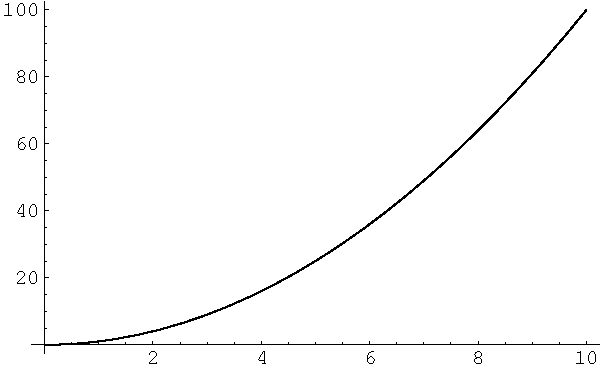
\includegraphics{gr-plot.pdf}
  \caption
  {%
    By default figures are not centered.
    This is a long caption to demonstrate that captions are single spaced.
    This is a long caption to demonstrate that captions are single spaced.%
  }
  \label{fi:not-centered}
\end{figure}
\end{VerbatimOut}

\MyIO


\begin{VerbatimOut}{z.out}

\MyRepeat{This is the second paragraph.  }{10}
\end{VerbatimOut}

\MyIO


\begin{VerbatimOut}{z.out}

\begin{figure}[ht]
  \centering
  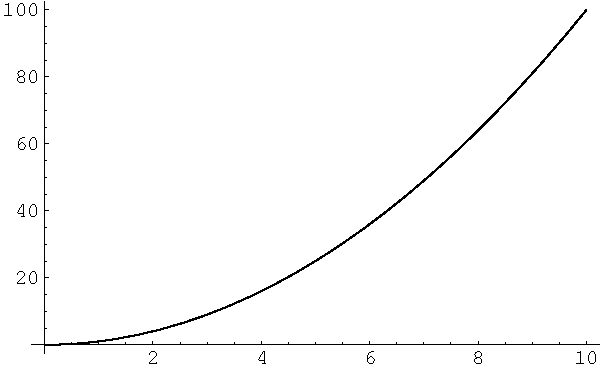
\includegraphics{gr-plot.pdf}
  \caption{Use {\tt \char'134centering\/} to center figures.}
  \label{fi:centered}
\end{figure}
\end{VerbatimOut}

\MyIO


\begin{VerbatimOut}{z.out}

\MyRepeat{This is the third paragraph.  }{15}
\end{VerbatimOut}

\MyIO


\begin{VerbatimOut}{z.out}

\begin{figure}[ht]
  \centering
  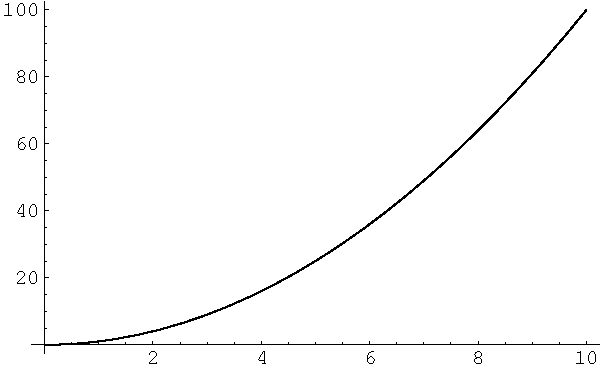
\includegraphics{gr-plot.pdf}
  \caption{This is another figuure.}
  \label{fi:another}
\end{figure}
\end{VerbatimOut}

\MyIO


\begin{VerbatimOut}{z.out}

\MyRepeat{This is the fourth paragraph.  }{10}
\end{VerbatimOut}

\MyIO


\begin{VerbatimOut}{z.out}
  
% See pages 4--5 of
%   http://mirrors.ibiblio.org/CTAN/macros/latex/contrib/caption/subcaption.pdf
% for how to use \subcaptionbox.
\begin{figure}[ht]
  % Center the entire figure (containing the two subfigures).
  \centering 
    % The \subcaptionbox for the first subfigure.
    \subcaptionbox
      % The first subcaption with a \label.
      % Use \ref{sf:two-parts-a} to print the subcaption number.
      {First subcaption.\label{sf:two-parts-a}}%
      % The first subfigure is this wide.
      [2in]%
      % This is the first subfigure.
      % You'll usually use an \includegraphics{filename}
      % inside the braces on the next line.
      {\bfseries First subfigure.}%
    % Put 0.5 inches of blank space between the subfigures.
    \hskip 0.5truein
    \subcaptionbox
      {Second subcaption.\label{sf:two-parts-b}}%
      [2in]%
      {\bfseries Second subfigure.}%
    % The caption for the entire figure (containing two subfigures).
    \caption{This figure has two parts.}
    % The label for the entire figure.
    \label{fi:two-parts}
\end{figure}
\end{VerbatimOut}

\MyIO


\begin{VerbatimOut}{z.out}

\MyRepeat{This is the fifth paragraph.  }{10}
\end{VerbatimOut}

\MyIO


\begin{VerbatimOut}{z.out}
  
\newpage

\begin{figure}[ht]
  \centering
    \subcaptionbox
      {First subcaption.\label{sf:four-parts-a}}
      [2in]%
      {\bfseries First subfigure.}%
    \hskip 0.5truein
    \subcaptionbox
      {Second subcaption.\label{sf:four-parts-b}}
      [2in]%
      {\bfseries Second subfigure.}%
    \vspace*{\baselineskip}
    \subcaptionbox
      {Third subcaption.\label{sf:four-parts-c}}
      [2in]%
      {\bfseries Third subfigure.}%
    \hskip 0.5truein
    \subcaptionbox
      {Fourth subcaption.\label{sf:four-parts-d}}
      [2in]%
      {\bfseries Fourth subfigure.}%
  \caption{This figure has four parts.}
  \label{fi:four-parts}
\end{figure}
\end{VerbatimOut}

\MyIO


\begin{VerbatimOut}{z.out}

\MyRepeat{This is the sixth paragraph.  }{10}
\end{VerbatimOut}

\MyIO


\begin{VerbatimOut}{z.out}

\newpage

\begin{figure}[ht]
  \centering 
    % Use a 5" font.
    {\fontsize{5in}{5in}\selectfont\(\hspace*{-0.07em}\sqrt 2\)}
    \caption{%
      A big ``\(\sqrt 2\)''.
      \LaTeX\ can make output big enough for T-shirts or posters.
      Square roots are printed with space before them,
      I put some negative horizontal space before this one to center it.%
    }
\end{figure}
\end{VerbatimOut}

\MyIO


\begin{figure}
  This is the figure.
  \caption{%
    Allocation to Common Edge for
    \(p(x_i) = 1-e^{-x_iz}\)% \frac{-x_i}z}\)%
  }
\end{figure}

\begin{VerbatimOut}{z.out}

\newpage

The remainder of this file tests having lots of figures.
There are 20 figures in this test.

\begin{figure}[ht]
  \centering
  
\includegraphics[scale=0.5]{gr-tally-01.pdf}
  \caption{Test figure 1 of 20.}
  \label{fi:1of20}
\end{figure}

\begin{figure}[ht]
  \centering
  
\includegraphics[scale=0.5]{gr-tally-02.pdf}
  \caption{Test figure 2 of 20.}
  \label{fi:2of20}
\end{figure}

\begin{figure}[ht]
  \centering
  
\includegraphics[scale=0.5]{gr-tally-03.pdf}
  \caption{Test figure 3 of 20.}
  \label{fi:3of20}
\end{figure}

\begin{figure}[ht]
  \centering
  
\includegraphics[scale=0.5]{gr-tally-04.pdf}
  \caption{Test figure 4 of 20.}
  \label{fi:4of20}
\end{figure}

\begin{figure}[ht]
  \centering
  
\includegraphics[scale=0.5]{gr-tally-05.pdf}
  \caption{Test figure 5 of 20.}
  \label{fi:5of20}
\end{figure}

\begin{figure}[ht]
  \centering
  
\includegraphics[scale=0.5]{gr-tally-06.pdf}
  \caption{Test figure 6 of 20.}
  \label{fi:6of20}
\end{figure}

\begin{figure}[ht]
  \centering
  
\includegraphics[scale=0.5]{gr-tally-07.pdf}
  \caption{Test figure 7 of 20.}
  \label{fi:7of20centered7}
\end{figure}

\begin{figure}[ht]
  \centering
  
\includegraphics[scale=0.5]{gr-tally-08.pdf}
  \caption{Test figure 8 of 20.}
  \label{fi:8of20}
\end{figure}

\begin{figure}[ht]
  \centering
  
\includegraphics[scale=0.5]{gr-tally-09.pdf}
  \caption{Test figure 9 of 20.}
  \label{fi:9of20}
\end{figure}

\begin{figure}[ht]
  \centering
  
\includegraphics[scale=0.5]{gr-tally-10.pdf}
  \caption{Test figure 10 of 20.}
  \label{fi:10of20}
\end{figure}

\begin{figure}[ht]
  \centering
  
\includegraphics[scale=0.5]{gr-tally-11.pdf}
  \caption{Test figure 11 of 20.}
  \label{fi:11of20}
\end{figure}

\begin{figure}[ht]
  \centering
  
\includegraphics[scale=0.5]{gr-tally-12.pdf}
  \caption{Test figure 12 of 20.}
  \label{fi:12of20}
\end{figure}

\begin{figure}[ht]
  \centering
  
\includegraphics[scale=0.5]{gr-tally-13.pdf}
  \caption{Test figure 13 of 20.}
  \label{fi:13of20}
\end{figure}

\begin{figure}[ht]
  \centering
  
\includegraphics[scale=0.5]{gr-tally-14.pdf}
  \caption{Test figure 14 of 20.}
  \label{fi:14of20}
\end{figure}

\begin{figure}[ht]
  \centering
  
\includegraphics[scale=0.5]{gr-tally-15.pdf}
  \caption{Test figure 15 of 20.}
  \label{fi:15of20}
\end{figure}

\begin{figure}[ht]
  \centering
  
\includegraphics[scale=0.5]{gr-tally-16.pdf}
  \caption{Test figure 16 of 20.}
  \label{fi:16of20}
\end{figure}

\begin{figure}[ht]
  \centering
  
\includegraphics[scale=0.5]{gr-tally-17.pdf}
  \caption{Test figure 17 of 20.}
  \label{fi:17of20}
\end{figure}

\begin{figure}[ht]
  \centering
  
\includegraphics[scale=0.5]{gr-tally-18.pdf}
  \caption{Test figure 18 of 20.}
  \label{fi:18of20}
\end{figure}

\begin{figure}[ht]
  \centering
  
\includegraphics[scale=0.5]{gr-tally-19.pdf}
  \caption{Test figure 19 of 20.}
  \label{fi:19of20}
\end{figure}

\begin{figure}[ht]
  \centering
  
\includegraphics[scale=0.5]{gr-tally-20.pdf}
  \caption{Test figure 20 of 20.}
  \label{fi:20of20}
\end{figure}
\end{VerbatimOut}

\MyIO


% Graphics.
%\ProvidesFile{ap-graphics.tex}[2021-08-23 graphics appendix]

\begin{VerbatimOut}{z.out}
\chapter{GRAPHICS}

There are many ways to make graphics for \LaTeX.
I like to use a system that uses \LaTeX\ fonts
so the appearance of the output is more professional.
\end{VerbatimOut}

\MyIO


\begin{VerbatimOut}{z.out}


\section{\LaTeX\ \TikZLogo\ package}
\index{TikZ@\TikZLogo}  
\end{VerbatimOut}

\MyIO


\begin{VerbatimOut}{z.out}


\subsection{Yin and yang}

This Yin and yang example was done by Thomas G. Kristensen \cite{kristensen}.
This is the ``traditional Taijitu symbol from Chinese philosophy''.\\
\ix{Kristensen, Thomas G.//Taijitu symbol//Yin and yang symbol}

\index{TikZ@\TikZLogo}  
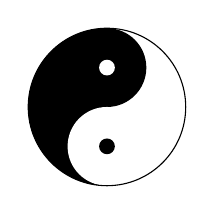
\begin{tikzpicture}
  % Yin and yang
  % Author: Thomas G. Kristensen
  
  % color one half of a unit circle                                              
  \begin{scope}
    \clip (0,0) circle (1cm);
    \fill[black] (0cm,1cm) rectangle (-1cm, -1cm);
  \end{scope}

  % fill heads                                                                   
  \fill[black] (0,0.5) circle (0.5cm);
  \fill[white] (0,-0.5) circle (0.5cm);

  % fill eyes                                                                    
  \fill[white] (0,0.5) circle (0.1cm);
  \fill[black] (0,-0.5) circle (0.1cm);

  % outer line                                                                   
  \draw (0,0) circle (1cm);

\end{tikzpicture}
\end{VerbatimOut}

\MyIO



\begin{VerbatimOut}{z.out}

\section{Mathematica (which uses Wolfram Language)}
\ix{Mathematica}
\end{VerbatimOut}

\MyIO


\begin{VerbatimOut}{z.out}

\section{MATLAB}
\ix{MATLAB}
\end{VerbatimOut}

\MyIO


\begin{VerbatimOut}{z.out}

\section{\protect\METAPOSTLogo\ (uses \LaTeX\ fonts)}
\index{METAPOST@\METAPOSTLogo}  

I did these \METAPOSTLogo\ \cite{metapost} examples
for Yanghyun Kim \cite{kim2009}.
\ix{Kim, Yanghyun}
\end{VerbatimOut}

\MyIO


\begin{VerbatimOut}{z.out}

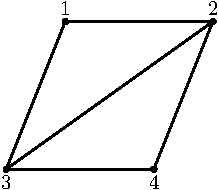
\includegraphics{gr-kim1.pdf}
\todoerror{need source code}  

\vspace{0.1truein}

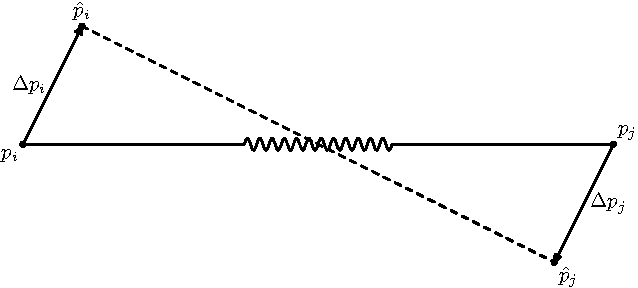
\includegraphics{gr-kim2.pdf}
\todoerror{need source code}  
\end{VerbatimOut}

\MyIO


\begin{VerbatimOut}{z.out}

\subsection{\METAPOSTLogo\ Tally Example}
\label{ss:tally-example}

Whenever I use files with numbers in them I like to put leading zeros
in the names so they will be listed in order in the directory.

These 20 graphics (gr-tally-01.pdf through gr-tally-20.pdf)

\vspace*{6pt}

{%
  % Let * represent zero or more spaces!
  % Method 1: \def\g#1{ requires using \g*{10} for 10.
  %           Two shifted characters, { and } are needed.
  % Method 2: \def\g#1/{ requires using \g*10/ for 10.
  %           One unshifted character, / is needed.
  \def\g#1/{\includegraphics[scale=0.5]{gr-tally-#1.pdf}}%

  % Note that tabular* instead of tabular is used below.
  %   The {\textwidth} makes the total width of the table the width
  % of the printed area of the page.
  %   The @{\kern2\parindent} puts blank space the width of two
  % paragraph indents before the first column.
  %   The @{extracolsep{\fill}} adds \fill space between all subsequent
  % columns.
  %   The lll left justifies the next three columns.
  % after the column.
  %   The @{\kern2\parindent} puts blank space the width of two
  % paragraph indents before the first column.
  \begin{tabular*}{\textwidth}{@{\kern2\parindent}@{\extracolsep{\fill}}lll@{\kern2\parindent}}%
    \g 01/& \g 02/& \g 03/\\
    \g 04/& \g 05/& \g 06/\\
    \g 07/& \g 08/& \g 09/\\
    \g 10/& \g 11/& \g 12/\\
    \g 13/& \g 14/& \g 15/\\
    \g 16/& \g 17/& \g 18/\\
    \g 19/& \g 20/\\
  \end{tabular*}%
}
\noindent were produced by

\MyI{misc/tally.mp}

\end{VerbatimOut}

\MyIO


\begin{VerbatimOut}{z.out}

\section{R}
\ix{R}
\end{VerbatimOut}

\MyIO


\begin{VerbatimOut}{z.out}

\section{\TikZLogo\ and PGF (uses \LaTeX\ fonts)}
\index{TikZ@\TikZLogo}
\ix{PGF}
\end{VerbatimOut}

\MyIO


\begin{VerbatimOut}{z.out}

\subsection{Clock}
\end{VerbatimOut}

\MyIO


\begin{VerbatimOut}{z.out}

The idea for this clock was originally
from a Google+ posting by
Afamefuna ``Ferdy'' Ibeabuchia.  \ix{Ibeabuchia, Afamefuna ``Ferdy''//PGF}
\index{TikZ@\TikZLogo}

\hbox to\textwidth{%
  \hfil
  \begin{tikzpicture}
    \def\CenterRadius{0.04cm}
    \def\InnerTickRadius{3.6cm}
    \def\OuterTickRadius{3.8cm}
    % Make \LR be an abbreviation for \LabelRadius so the
    % lines below will fit within the width of the page.
    \def\LabelRadius{4.5cm}      \let\LR=\LabelRadius
    \def\HourHandRadius{2.5cm}   \def\HourHandBase{0.3cm}
    \def\MinuteHandRadius{3cm}   \def\MinuteHandBase{0.4cm}
    \def\SecondHandRadius{3.5cm} \def\SecondHandBase{0.5cm}
    \def\DS{\displaystyle}
    \fill (0,0) circle (\CenterRadius);
    \foreach \i in {0,30,...,330}
    \draw (\i:\InnerTickRadius)--(\i:\OuterTickRadius);
    \node at (  0:\LR) {$\DS \qquad \sqrt9 + 9 - 9$};        %  3
    \node at ( 30:\LR) {$\DS \frac{9+9}9$};                  %  2
    \node at ( 60:\LR) {$\DS \frac{\sqrt9\sqrt9}9$};         %  1
    \node at ( 90:\LR) {$\DS 9 + \frac9{\sqrt9}$};           % 12
    \node at (120:\LR) {$\DS \frac{99}9$};                   % 11
    \node at (150:\LR) {$\DS 9 + \frac99$};                  % 10
    \node at (180:\LR) {$\DS \sqrt[\scriptstyle 9]{9^9}$};   %  9
    \node at (210:\LR) {$\DS 9 - \frac99$};                  %  8
    \node at (240:\LR) {$\DS 9 - \sqrt9 + \lceil.9\rceil$};  %  7
    \node at (270:\LR) {$\DS 9 - \frac9{\sqrt9}$};           %  6
    \node at (300:\LR) {$\DS \sqrt9\,! - \frac99$};          %  5
    \node at (330:\LR) {$\DS \sqrt9 + \frac99$};             %  4
    % In the following
    %   ABBREVIATION    DESCRIPTION
    %   deg             degrees
    %   min             minutes
    %   sec             seconds
    % for second hand:
    %   (9 sec/60 sec) * 360 deg = 54 deg;
    %   90 deg - 54 deg = 36 deg
    \draw[rotate around={36:(0,0)}]
      (-\SecondHandBase,\SecondHandBase) -- (\SecondHandRadius,0)
        -- (-\SecondHandBase,-\SecondHandBase) -- cycle;
    % for minute hand:
    %   (9 min/60 min) * 360 deg = 54 deg;
    %   90 deg - 54 deg = 36 deg
   \draw[rotate around={36:(0,0)}]
     (-\MinuteHandBase,\MinuteHandBase) -- (\MinuteHandRadius,0)
       -- (-\MinuteHandBase,-\MinuteHandBase) -- cycle;
    % for hour hand:
    %   (9 min * (60 sec/1 min)) + 9 sec) / 3600 sec
    %     = 549 sec / 3600 sec = 0.1525
    %   The hour hand is 0.1525 of the way from 9:00 to 10:00.
    %   Each hour is 30 degrees on the clock, so the hour hand
    %   position is
    %     30 deg * 0.1525 = 4.575 deg past 9:00
    %   180 deg - 4.575 deg = 175.425 deg
    \draw[rotate around={175.425:(0,0)}]
      (-\HourHandBase,\HourHandBase) -- (\HourHandRadius,0)
      -- (-\HourHandBase,-\HourHandBase) -- cycle;
  \end{tikzpicture}
  \hfil
}
\end{VerbatimOut}

\MyIO


\begin{VerbatimOut}{z.out}

\subsection{Glider}
\ix{Hirzel, Alex//Glider emblem representing the hacker community}

The glider
is a pattern from the Game of Life,
and it's used as an emblem representing the hacker community.

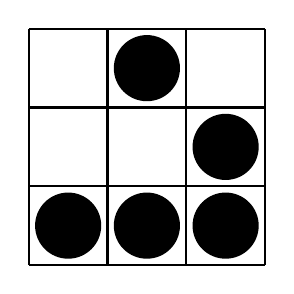
\begin{tikzpicture}[thick]
  \draw (0,0) grid (3,3);
  \foreach \c in {(0,0), (1,0), (2,0), (2,1), (1,2)}
    \fill \c + (0.5,0.5) circle (0.42);
\end{tikzpicture}
\end{VerbatimOut}

\MyIO


% Numbers and Units.
%\ProvidesFile{ap-numbers-and-units.tex}[2021-08-23 numbers and units appendix]

%  Primary sources:
%      See https://www.bipm.org/utils/common/pdf/si-brochure/SI-Brochure-9-EN.pdf.
%      See https://www.nist.gov/pml/special-publication-811/nist-guide-si-chapter-4-two-classes-si-units-and-si-prefixes.
%
%  Notes:
%      See https://www.iso.org/standard/60241.html.

% Historic Vote Ties Kilogram and Other Units to Natural Constants
% NIST
% https://www.nist.gov/news-events/news/2018/11/historic-vote-ties-kilogram-and-other-units-natural-constants
% created 2018-11-16
% updated 2018-12-21
% last retrieved 2018-12-22

% https://www.bipm.org/utils/common/pdf/CGPM-2018/26th-CGPM-Resolutions.pdf
% Resolutions adopted
% 26^e CGPM
% Versailes
% 13--16 November 2018
% last retrieved 2018-12-30

% author Joseph Wright
% date 2018-05-17
% retrieved 2018-12-29
% url ftp://ftp.dante.de/tex-archive/macros/latex/exptl/siunitx/siunitx.pdf


\begin{VerbatimOut}{z.out}
\chapter{NUMBERS AND UNITS}
\end{VerbatimOut}

\MyIO


\begin{VerbatimOut}{z.out}

Note to self: scientific prefixes, scientific suffixes, tables.

The puthesis 2.0 and after documentclass uses the siunitx
package with some extra definitions in the puthesis.cls
file to do numbers and units.
\end{VerbatimOut}

\MyIO


\begin{VerbatimOut}{z.out}

\section{Number Examples}
\end{VerbatimOut}

\MyIO


\begin{VerbatimOut}{z.out}
\noindent\begin{tabular}{@{}lll@{}}
  \bfseries Input& \bfseries Output& \bfseries Comment\\
  \tabularspace
  \verb+\num{-0.12345}+& \num{-0.12345}& note the small space after the ``3''\\
  \verb+\num{-0.1234}+&
    \num{-0.1234}&
    note no space between the ``3'' and ``4''\\
  \verb+\num{-.123}+& \num{-.123}& the ``0.'' is inserted automatically\\
  \verb+\num{123}+& \num{123}\\
  \verb+\num{1234}+& \num{1234}\\
  \verb+\num{12345}+& \num{12345}& note the small space after the ``2''\\
  \verb+\num{2e4}+& \num{2e4}\\
  \verb+\num{e5}+& \num{e5}\\
  \verb+\num{2.34567e6}+&
    \num{2.34567e6}&
    note the small space after the ``5''\\
\end{tabular}
\end{VerbatimOut}

\MyIO


\begin{VerbatimOut}{z.out}

\section{Unit Examples}
\end{VerbatimOut}

\MyIO


\begin{VerbatimOut}{z.out}

See page~\pageref{se:Complete-List-of-Units}
for the complete list
of units defined by \PurdueThesisLogo.

\noindent\begin{tabular}{@{}lll@{}}
  \bfseries Input& \bfseries Output& \bfseries Comment\\
  \tabularspace
  \verb+\si{\kg}+& \si{\kg}& kilogram\\
  \verb+\si{\m}+& \si{\m}& meter\\
  \verb+\si{\kg\per\m\squared}+&
    \si{\kg\per\m\squared}&
    \(= \si{\kg}/\si{\m\squared}\)\\
\end{tabular}
\end{VerbatimOut}

\MyIO


\begin{VerbatimOut}{z.out}

\section{Combined Number and Unit Examples}
\end{VerbatimOut}

\MyIO


\begin{VerbatimOut}{z.out}
\begin{tabular}{@{}lll@{}}
  \bfseries Input& \bfseries Output& \bfseries Comment\\
  \tabularspace
  \verb+\SI{12}{\kg}+& \SI{12}{\kg}& 12 kilograms\\
  \verb+\SI{34}{\m}+&  \SI{34}{\m}& 34 meters\\
  % The next input line is too wide for the margins
  % so I'm splitting it into pieces.
  \verb+\SI{4.5e3}{\kg\per\m\squared}+&
    \SI{4.5e3}{\kg\per\m\squared}&
    \(= \num{4.5e3}\,\si{\kg}/\si{\m\squared}\)\\
\end{tabular}
\end{VerbatimOut}

\MyIO


\begin{VerbatimOut}{z.out}

How many seconds are in a non-leap year that does not have any leap seconds?
% I tried several things and couold not get \cancel to work with \per.
% Mark Senn    2019-12-29
\begin{align*}
           \frac{\SI{365}{\cancel\d}}{\si{\y}}
    \times \frac{\SI{24}{\cancel\h}}{\si{\cancel\d}}
    \times \frac{\SI{60}{\cancel\min}}{\si{\cancel\h}}         
    \times \frac{\SI{60}{\s}}{\si{\cancel\min}}         
    % From http://www.emerson.emory.edu/services/latex/latex_119.html
    %     Spacing in Math Mode
    %     In a math environment, LaTeX ignores the spaces you type
    %     and puts in the spacing that it thinks is best. LaTeX formats
    %     mathematics the way it's done in mathematics texts. If you
    %     want different spacing, LaTeX provides the following four
    %     commands for use in math mode:
    %         \; - a thick space
    %         \: - a medium space
    %         \, - a thin space
    %         \! - a negative thin space
    & = \num{31536000}\;\frac{\si{\s}}{\si{\y}}\\
    & = \SI{31536000}{\s\per\y}\\
    & \approx \SI{3e7}{\s\per\y}\\
    & \approx \text{30 million\,}\si{\s\per\y}\\
\end{align*}
\end{VerbatimOut}

\MyIO


\begin{VerbatimOut}{z.out}

\section{Binary Prefixes}
\end{VerbatimOut}

\MyIO


\begin{VerbatimOut}{z.out}

The \verb+\kibi+ \ldots \verb+\yobi+
commands are defined immediately after the \verb+\usepackage{siunitx}+ command
in the PurdueThesis.cls file.
\end{VerbatimOut}

\MyIO


\begin{VerbatimOut}{z.out}

\newcolumntype{m}{>{$}r<{$}}  % math mode version of "r" column type
\renewcommand{\t}[4]{\(2^{#1}\) bytes is a #2, \(10^{#3}\) bytes is a #4}
\begin{tabular}{@{}mllll@{}}
  \multicolumn{1}{l}{\bfseries Power}&
    \bfseries Prefix&
    \bfseries Symbol&
    \bfseries Command&
    \bfseries Comment\\
  \tabularspace
  10& kibi& \unit{\kibi\nounit}& \verb+\si{\kibi}+& \t{10}{KB}{3}{KiB}\\
  20& mebi& \unit{\mebi\nounit}& \verb+\si{\mebi}+& \t{20}{MB}{6}{MiB}\\
  30& gibi& \unit{\gibi\nounit}& \verb+\si{\gibi}+& \t{30}{GB}{9}{GiB}\\
  40& tebi& \unit{\tebi\nounit}& \verb+\si{\tebi}+& \t{40}{TB}{12}{TiB}\\
  50& pebi& \unit{\pebi\nounit}& \verb+\si{\pebi}+& \t{50}{PB}{15}{PiB}\\
  60& exbi& \unit{\exbi\nounit}& \verb+\si{\exbi}+& \t{60}{EB}{18}{EiB}\\
  70& zebi& \unit{\zebi\nounit}& \verb+\si{\zebi}+& \t{70}{ZB}{21}{ZiB}\\
  80& yobi& \unit{\yobi\nounit}& \verb+\si{\yobi}+& \t{80}{YB}{24}{YiB}\\
\end{tabular}
\end{VerbatimOut}

\MyIO


\begin{VerbatimOut}{z.out}

\section{Decimal Prefixes}
\end{VerbatimOut}

\MyIO

\begin{VerbatimOut}{z.out}

\newcolumntype{m}{>{$}r<{$}}  % math mode version of "r" column type
\begin{tabular}{@{}mllll@{}}
  \multicolumn{1}{l}{\bfseries Power}&
    \bfseries Prefix&
    \bfseries Symbol&
    \bfseries Command&
    \bfseries Comment\\
  \tabularspace
  -24& yocto& \unit{\yocto\nounit}& \verb+\si{\yocto}+\\
  -21& zepto& \unit{\zepto\nounit}& \verb+\si{\zepto}+\\
  -18& atto&  \unit{\atto\nounit}&  \verb+\si{\atto}+\\
  -15& femto& \unit{\femto\nounit}& \verb+\si{\femto}+\\
  -12& pico&  \unit{\pico\nounit}&  \verb+\si{\pico}+\\
   -9& nano&  \unit{\nano\nounit}&  \verb+\si{\nano}+\\
   -6& micro& \unit{\micro\nounit}& \verb+\si{\micro}+\\
   -3& milli& \unit{\milli\nounit}& \verb+\si{\milla}+\\
   -2& centi& \unit{\centi\nounit}& \verb+\si{\centi}+\\
   -1& deci&  \unit{\deci\nounit}&  \verb+\si{\deci}+\\
    1& deca&  \unit{\deca\nounit}&  \verb+\si{\deca}+\\
    1& deka&  \unit{\deka\nounit}&  \verb+\si{\deka}+& same as \verb+\si{\deca}+\\
    2& hecto& \unit{\hecto\nounit}& \verb+\si{\hecto}+\\
    3& kilo&  \unit{\kilo\nounit}&  \verb+\si{\kilo}+\\
    6& mega&  \unit{\mega\nounit}&  \verb+\si{\mega}+\\
    9& giga&  \unit{\giga\nounit}&  \verb+\si{\giga}+\\
   12& tera&  \unit{\tera\nounit}&  \verb+\si{\tera}+\\
   15& peta&  \unit{\peta\nounit}&  \verb+\si{\peta}+\\
   18& exa&   \unit{\exa\nounit}&   \verb+\si{\exa}+\\
   21& zetta& \unit{\zetta\nounit}& \verb+\si{\zetta}+\\
   24& yotta& \unit{\yotta\nounit}& \verb+\si{\yotta}+\\
\end{tabular}
\end{VerbatimOut}

\MyIO


\begin{VerbatimOut}{z.out}

\section{SI Units}
\end{VerbatimOut}

\MyIO


\begin{VerbatimOut}{z.out}

The International System of Units
(SI)
% !!! Doing
% !!!     \include{tipa}
% !!! in thesis.tex so \textprimstress works
% !!! apparently causes problems with math commands.
% !!! Figure out why the following doesn't work later.
% (%
%   SI,
%   abbreviated from the French Syst\`eme International
%   (d\textprimstress unit\'es)%
% )
is the modern form of the metric system.
There are seven SI base units:

\hspace{40pt}
\begin{tabular}{@{}lll@{}}
  \tabularspace
  \bfseries Name& \bfseries Unit Of&         \bfseries Symbol\\
  \tabularspace
  ampere&         electrical current&        \si{\ampere}\\
  candela&        luminous intensity&        \si{\candela}\\
  kelvin&         thermodynamic temperature& \si{\kelvin}\\
  kg&             mass&                      \si{\kilogram}\\
  meter&          length&                    \si{\meter}\\
  mole&           amount of substance&       \si{\mole}\\
  second&         time&                      \si{\second}\\
\end{tabular}
\end{VerbatimOut}

\MyIO


\begin{VerbatimOut}{z.out}

\section{Complete List of Units}
\label{se:Complete-List-of-Units}
\end{VerbatimOut}

\MyIO

\begin{VerbatimOut}{z.out}

{%
  \ZZbaselinestretch{1}
  \newcommand\vsp{\noalign{\vspace*{6pt}}}
  % From
  % https://tex.stackexchange.com/questions/31508/flushleft-with-p-option-in-tabular
  %     It's necessary to use the \arraybackslash in the last column,
  %     otherwise \\ would not end the table row.  You can use \newline
  %     to end lines in the last column cells (and the regular \\ in
  %     the other column cells).
  %     ...
  %     If you need it often, consider defining a new column type using
  %     array features, as I did here:
  %         \newcolumntype{P}[1]{>{\raggedright\arraybackslash}p{#1}}
  \newcolumntype{P}[1]{>{\raggedright\arraybackslash}p{#1}}%
% \begin{longtable}{@{}P{1.4in}P{1in}llP{1.8in}@{}}
% \begin{longtable}{@{}P{1in}P{1in}llP{1.8in}@{}}
% \begin{longtable}{@{}P{1.2in}P{1in}llP{1.8in}@{}}
% \begin{longtable}{@{}P{90.72pt}P{1in}llP{1.8in}@{}}  % 1.2in (86.72pt) + 4pt = 90.72pt
  \begin{longtable}{@{}P{1.4in}P{1in}llP{1.8in}@{}}% 1.2in (86.72pt) + 4pt = 90.72pt
      \caption{Units and Corresponding Symbols}\\
      \bfseries Name&
        \bfseries Unit Of&
        \bfseries Symbol&
        \bfseries Command&
        \bfseries Is equal to\\
      \vsp
    \endfirsthead
      \caption[]{~\emph{continued}}\\
      \bfseries Name&
        \bfseries Unit Of&
        \bfseries Symbol&
        \bfseries Command&
        \bfseries Is equal to\\
      \vsp
    \endhead
      \vsp
      % I don't know why the \hspace*{-7.5mm} was
      % needed to center this horizontally.
      \multicolumn{5}{@{}c@{}}{\hspace*{-7.5mm}\emph{continued on next page}}%
    \endfoot    
    \endlastfoot
    ampere&
      electrical current&
      \si{\A}&
      \verb+\si{\A}+&
      (SI base unit)\\
    \quad picoampere&
      \ditto&
      \si{\pA}&
      \verb+\si{\pA}+&
      \SI{e-12}{\A}\\ 
    \quad nanoampere&
      \ditto&
      \si{\nA}&
      \verb+\si{\nA}+&
      \SI{e-9}{\A}\\
    \quad microampere&
      \ditto&
      \si{\uA}&
      \verb+\si{\uA}+&
      \SI{e-6}{\A}\\
    \quad milliampere&
      \ditto&
      \si{\mA}&
      \verb+\si{\mA}+&
      \SI{e-3}{\A}\\
    \quad kiloampere&
      \ditto&
      \si{\kA}&
      \verb+\si{\kA}+&
      \SI{e3}{\A}\\
    \vsp
    % \aa ngstr\"om&
    %   length&
    %   \si{\AA}&
    %   \verb+\si{\AA}+&
    %   \SI{e-10}{\m}\\
    \vsp
    arcminute&
      plane angle&
      \si{\arcmin}&
      \verb+\si{\arcmin}+&
      % Changed
      %     \SI{1/60}{\degree}\\
      % to
      1/60\unit{\degree\nounit}\\
    arcsecond&
      plane angle&
      \si{\arcsec}&
      \verb+\si{\arcsec}+&
      % Changed
      %     \SI{1/60}{\arcmin}\\
      % to
      1/60\unit{\arcmin\nounit}\\
    \vsp
    astronomical unit&
      length&
      \si{\au}&
      \verb+\si{\au}+&
      mean earth to\newline sun distance\\
    \vsp
    % From
    %     siunitx - A comprehensive (SI) units package
    %     Joseph Wright
    %     Released 2021-08-04
    %     (this describes v3.0.24, last revised 2021-08-04)
    %     https://mirror.las.iastate.edu/tex-archive/macros/latex/contrib/siunitx/siunitx.pdf
    % page 51:
    %     ...the unit \atomicmassunit has similar deprecated status:
    %     this was listed as with experimentally-determined units
    %     in the 8th Edition of the si Brochure but is equivalent
    %     to the dalton, a unit which remains accepted.
    % atomic mass unit&
    %   mass&
    %   \si{\amu}&
    %   \verb+\si{\amu}+&
    %   \(1/12\) mass of\newline carbon-12 atom\\
    % \vsp
    bar&
      pressure&
      \si{\bar}&
      \verb+\si{\bar}+&
      \SI{e-5}{\Pa}\\
    \quad millibar&
      \ditto&
      \si{\mbar}&
      \verb+\si{\mbar}+&
      \SI{e-3}{\bar}\\
    \vsp
    barn&
      area&
      \si{\b}&
      \verb+\si{\b}+&
      \SI{e-28}{\m\squared}\\
    \vsp
    becquerel&
      radioactivity&
      \si{\Bq}&
      \verb+\si{\Bq}+&
      one radioactive\newline decay per second\\
    \vsp
    bel&
      sound intensity&
      \si{\B}&
      \verb+\si{\B}+&
      10 decibels\\
    \quad decibel&
      \ditto&
      \si{\dB}&
      \verb+\si{\dB}+&
      \SI{e-1}{\B}\\
    \vsp
    bohr&
      length&
      \si{\bohr}&
      \verb+\si{\bohr}+&
      distance between\newline nucleus and electron\newline in hydrogen atom\\
    \vsp
    bushel&
      quantity&
      \si{\bu}&
      \verb+\si{\bu}+&
      see \cite{wikipedia-bushel}\\
    \vsp
    candela&
      luminous intensity&
      \si{\cd}&
      \verb+\si{\cd}+&
      (SI base unit)\\
    \vsp
    coulomb&
      electrical charge&
      \si{\C}&
      \verb+\si{\C}+&
      \si{\A\per\s}\\
    \vsp
    dalton&
      mass&
      \si{\Da}&
      \verb+\si{\Da}+&
      another name for\newline atomic mass unit\\
    \vsp
    day&
      time&
      \si{\d}&
      \verb+\si{\d}+&
      \SI{86400}{\s}\\
    \vsp
    degree&
      plane angle&
      \si{\degree}&
      \verb+\si{\degree}+&
      1/360 of a cicle\\
    \vsp
    degree Celsius&
      temperature&
      \si{\celsius}&
      \verb+\si{\celsius}+&
      xxx\\
    \vsp
    electron mass&
      mass&
      \si{\em}&
      \verb+\si{\em}+&
      xxx\\
    \vsp
    electronvolt&
      energy&
      \si{\eV}&
      \verb+\si{\eV}+&
      xxx\\
    \quad millielectronvolt&
      \ditto&
      \si{\meV}&
      \verb+\si{meV}+&
      \SI{e-3}{\eV}\\
    \quad kiloelectronvolt&
      \ditto&
      \si{\keV}&
      \verb+\si{keV}+&
      \SI{e3}{\eV}\\
    \quad megaelectronvolt&
      \ditto&
      \si{\MeV}&
      \verb+\si{MeV}+&
      \SI{e6}{\eV}\\
    \quad gigaelectronvolt&
      \ditto&
      \si{\GeV}&
      \verb+\si{\GeV}+&
      \SI{e9}{\eV}\\
    \quad teraelectronvolt&
      \ditto&
      \si{\TeV}&
      \verb+\si{\TeV}+&
      \SI{e12}{\eV}\\
    \vsp
    elementary charge&
      electrical charge&
      \si{\ec}&
      \verb+\si{\ec}+&
      \href{https://en.wikipedia.org/wiki/Elementary_charge}{\SI{\approx 1.6e19}{\C}}\\
    \vsp
    farad&
      electrical capacitance&
      \si{\F}&
      \verb+\si{\F}+&
      \si{\s\tothe{4}\A\squared\per\m\squared\per\kg}\\
    \quad femtofarad&
      \ditto&
      \si{\fF}&
      \verb+\si{\fF}+&
      \SI{e-15}{\F}\\
    \quad picofarad&
      \ditto&
      \si{\pF}&
      \verb+\si{\pF}+&
      \SI{e-12}{\F}\\
    \vsp
    foot&
      length&
      \si{\ft}&
      \verb+\si{\ft}+&
      \SI{0.3048}{\m}\\  % not an SI unit
    \vsp
    % gauss: The gauss, symbol G, sometimes Gs, is the cgs unit of measurement of magnetic flux.
    gray&
      absorbed dose of ionizing radiation&
      \si{\Gy}&
      \verb+\si{\Gy}+&
      \si{\J\per\kg}\\
    \vsp
    hartree&
      energy used in molecular orbital calculations&
      \si{\hartree}&
      \verb+\si{\hartree}+&
      xxx\\
    \vsp
    hectare&
      area&
      \si{\ha}&
      \verb+\si{\ha}+&
      \SI{e4}{\m\squared}\\
    \vsp
    henry&
      electrical inductance&
      \si{\H}&
      \verb+\si{\H}+&
      \si{\kg\m\squared\per\s\squared\per\A\squared}\\
    \vsp
    hertz&
      frequency&
      \si{\Hz}&
      \verb+\si{\Hz}+&
      \si{\per\s}\\
    \quad millihertz&
      \ditto&
      \si{\mHz}&
      \verb+\si{\mHz}+&
      \SI{e-3}{\Hz}\\
    \quad kilohertz&
      \ditto&
      \si{\kHz}&
      \verb+\si{\kHz}+&
      \SI{e3}{\Hz}\\
    \quad megahertz&
      \ditto&
      \si{\MHz}&
      \verb+\si{\MHz}+&
      \SI{e6}{\Hz}\\
    \quad gigahertz&
      \ditto&
      \si{\GHz}&
      \verb+\si{\GHz}+&
      \SI{e9}{\Hz}\\
    \quad terahertz&
      \ditto&
      \si{\THz}&
      \verb+\si{\THz}+&
      \SI{e12}{\Hz}\\
    \vsp
    horsepower&
      power&
      \si{\hp}&
      \verb+\si{\hp}+&
      \SI{\approx 745.7}{\W}, {\bfseries IMPORTANT:\newline
        see \href{https://en.wikipedia.org/wiki/Horsepower#Mechanical_horsepower}{Horsepower}}\\
        % not an SI unit
    \vsp
    hour&
      time&
      \si{\h}&
      \verb+\si{\h}+&
      \SI{3600}{\s}\\
    \vsp
    inch&
      length&
      \si{\in}&
      \verb+\si{\in}+&
      \SI{25.4}{\mm}\\  % not an SI unit
    \vsp
    joule&
      work or energy&
      \si{\J}&
      \verb+\si{\J}+&
      \si{\kg\m\squared\per\s\squared}\\
    \quad microjoule&
      \ditto&
      \si{\uJ}&
      \verb+\si{\uJ}+&
      \SI{e-6}{\J}\\
    \quad millijoule&
      \ditto&
      \si{\mJ}&
      \verb+\si{\mJ}+&
      \SI{e-3}{\J}\\
    \quad kilojoule&
      \ditto&
      \si{\kJ}&
      \verb+\si{\kJ}+&
      \SI{e3}{\J}\\
    \quad megajoule&
      \ditto&
      \si{\MJ}&
      \verb+\si{\MJ}+&
      \SI{e6}{\J}\\
    \vsp
    katal&
      catalytic activity&
      \si{\kat}&
      \verb+\si{\kat}+&
      \si{\mol\per\s}\\
    \vsp
    kelvin&
      thermodynamic temperature&
      \si{\K}&
      \verb+\si{\K}+&
      (SI base unit)\\
    \vsp
    kilogram&
      mass&
      \si{\kg}&
      \verb+\si{\kg}+&
      (SI base unit)\\
    \quad femtogram&
      \ditto&
      \si{\fg}&
      \verb+\si{\fg}+&
      \SI{e-15}{\g}\\
    \quad picogram&
      \ditto&
      \si{\pg}&
      \verb+\si{\pg}+&
      \SI{e-12}{\g}\\
    \quad nanogram&
      \ditto&
      \si{\ng}&
      \verb+\si{\ng}+&
      \SI{e-9}{\g}\\
    \quad microgram&
      \ditto&
      \si{\ug}&
      \verb+\si{\ug}+&
      \SI{e-6}{\g}\\
    \quad milligram&
      \ditto&
      \si{\mg}&
      \verb+\si{\mg}+&
      \SI{e-3}{\g}\\
    \quad gram&
      \ditto&
      \si{\g}&
      \verb+\si{\g}+&
      \SI{e-3}{\kg}\\
    \vsp
    kilowatt hour&
      electrical energy&
      \si{\kWh}&
      \verb+\si{\kWh}+&
      \si{\kW\h}\\
    \vsp
    knot&
      speed&
      \si{\kn}&
      \verb+\si{\kn}+&
      \si{\M\per\h}\\
    \vsp
    liter&
      volume&
      \si{\L}&
      \verb+\si{\L}+&
      \SI{e-3}{m\cubed}\\
    \quad microliter&
      \ditto&
      \si{\uL}&
      \verb+\si{\uL}+&
      \SI{e-6}{\L}\\
    \quad milliliter&
      \ditto&
      \si{\mL}&
      \verb+\si{\mL}+&
      \SI{e-3}{\L}\\
    \quad hectoliter&
      \ditto&
      \si{\hL}&
      \verb+\si{\hL}+&
      \SI{e2}{\L}\\
    \vsp
    lumen&
      luminous flux&
      \si{\lm}&
      \verb+\si{\lm}+&
      \si{\cd\sr}\\
    \vsp
    lux&
      illumination&
      \si{\lx}&
      \verb+\si{\lx}+&
      \si{\lm\per\m\squared}\\
    \vsp
    meter&
      length&
      \si{\m}&
      \verb+\si{\m}+&
      (SI base unit)\\
    \quad picometer&
      \ditto&
      \si{\pm}&
      \verb+\si{\pm}+&
      \SI{e-12}{\m}\\
    \quad nanometer&
      \ditto&
      \si{\nm}&
      \verb+\si{\nm}+&
      \SI{e-9}{\m}\\
    \quad micrometer&
      \ditto&
      \si{\um}&
      \verb+\si{\um}+&
      \SI{e-6}{\m}\\
    \quad millimeter&
      \ditto&
      \si{\mm}&
      \verb+\si{\mm}+&
      \SI{e-3}{\m}\\
    \quad centimeter&
      \ditto&
      \si{\cm}&
      \verb+\si{\cm}+&
      \SI{e-2}{\m}\\
    \quad decimeter&
      \ditto&
      \si{\dm}&
      \verb+\si{\dm}+&
      \SI{e-1}{\m}\\
    \quad kilometer&
      \ditto&
      \si{\km}&
      \verb+\si{\km}+&
      \SI{e3}{\m}\\
    \vsp
    % mile: not an SI unit
    millimeter of mercury&
      pressure&
      \si{\mmHg}&
      \verb+\si{\mmHg}+&
      \href{https://en.wikipedia.org/wiki/Millimetre_of_mercury}{\SI{\approx 133}{\Pa}}\\
    \vsp
    minute&
      time&
      \si{\min}&
      \verb+\si{\min}+&
      \SI{60}{\s}\\
    \vsp
    mole&
      amount of substance&
      \si{\mol}&
      \verb+\si{\mol}+&
      (SI base unit)\\
    \quad femtomole&
      \ditto&
      \si{\fmol}&
      \verb+\si{\fmol}+&
      \SI{e-15}{\mol}\\
    \quad picomole&
      \ditto&
      \si{\pmol}&
      \verb+\si{\pmol}+&
      \SI{e-12}{\mol}\\
    \quad nanomole&
      \ditto&
      \si{\nmol}&
      \verb+\si{\nmol}+&
      \SI{e-9}{\mol}\\
    \quad micromole&
      \ditto&
      \si{\umol}&
      \verb+\si{\umol}+&
      \SI{e-6}{\mol}\\
    \quad millimole&
      \ditto&
      \si{\mmol}&
      \verb+\si{\mmol}+&
      \SI{e-3}{\mol}\\
    \quad kilomole&
      \ditto&
      \si{\kmol}&
      \verb+\si{\kmol}+&
      \SI{e3}{\mol}\\
    \vsp
    nautical mile&
      distance&
      \si{\M}&
      \verb+\si{\M}+&
      \SI{1852}{\m}\\
    \vsp
    neper&
      gain, loss, and relative values&
      \si{\Np}&
      \verb+\si{\Np}+&
      1\\
    \vsp
    newton&
      force&
      \si{\N}&
      \verb+\si{\N}+&
      \si{\kg\m\per\s\squared}\\
    \quad millinewton&
      \ditto&
      \si{\mN}&
      \verb+\si{\mN}+&
      \SI{e-3}{\N}\\
    \quad kilonewton&
      \ditto&
      \si{\kN}&
      \verb+\si{\kN}+&
      \SI{e3}{\N}\\
    \quad meganewton&
      \ditto&
      \si{\MN}&
      \verb+\si{\MN}+&
      \SI{e6}{\N}\\
    \vsp
    ohm&
      electrical resistance&
      \si{\ohm}&
      \verb+\si{\ohm}+&
      \si{\kg\m\squared\per\s\cubed\per\A\squared}\\
    \quad milliohm&
      \ditto&
      \si{\mohm}&
      \verb+\si{\mohm}+&
      \SI{e-3}{ohm}\\
    \quad kiloohm&
      \ditto&
      \si{\kohm}&
      \verb+\si{\kohm}+&
      \SI{e3}{ohm}\\
    \quad megaohm&
      \ditto&
      \si{\Mohm}&
      \verb+\si{\Mohm}+&
      \SI{e6}{ohm}\\
    \vsp
    pascal&
      pressure&
      \si{\Pa}&
      \verb+\si{\Pa}+&
      \si{\kg\per\m\per\s\squared}\\
    \qquad kilopascal&
      \ditto&
      \si{\kPa}&
      \verb+\si{\kPa}+&
      \SI{e3}{\Pa}\\
    \qquad megapascal&
      \ditto&
      \si{\MPa}&
      \verb+\si{\MPa}+&
      \SI{e6}{\Pa}\\
    \qquad gigapascal&
      \ditto&
      \si{\GPa}&
      \verb+\si{\GPa}+&
      \SI{e9}{\Pa}\\
    \vsp
    percent&
      hundredths&
      \si{\percent}&
      \verb+\si{\percent}+&
      \SI{e-2}{}\\
    \vsp
    pound&
      weight&
      \si{\lb}&
      \verb+\si{\lb}+&
      \SI{.45359237}{\kg}\\  % not an SI unit
    \vsp
    radian&
      plane angular measurement&
      \si{\rad}&
      \verb+\si{\rad}+&
      \(180/\pi\) \unit{\degree\nounit}\\
    \vsp
    reduced Planck constant&
      angular momentum&
      \si{\planckbar}&
      \verb+\si{\planckbar}+&
      \(\approx \SI{1.05e-34}{\J\s}\)\\
    \vsp
    second&
      time&
      \si{\s}&
      \verb+\si{\s}+&
      (SI base unit)\\
    \quad attosecond&
      \ditto&
      \si{\as}&
      \verb+\si{\as}+&
      \SI{e-18}{\s}\\
    \quad femtosecond&
      \ditto&
      \si{\fs}&
      \verb+\si{\fs}+&
      \SI{e-15}{\s}\\
    \quad picosecond&
      \ditto&
      \si{\ps}&
      \verb+\si{\ps}+&
      \SI{e-12}{\s}\\
    \quad nanosecond&
      \ditto&
      \si{\ns}&
      \verb+\si{\ns}+&
      \SI{e-9}{\s}\\
    \quad microsecond&
      \ditto&
      \si{\us}&
      \verb+\si{\us}+&
      \SI{e-6}{\s}\\
    \quad millisecond&
      \ditto&
      \si{\ms}&
      \verb+\si{\ms}+&
      \SI{e-3}{\s}\\
    \vsp
    siemens&
      conductance&
      \si{\S}&
      \verb+\si{\S}+&
      \si{\per\kg\per\m\squared\s\cubed\A\squared}\\
    \vsp
    sievert&
      dosage of ionizing radiation&
      \si{\Sv}&
      \verb+\si{\Sv}+&
      \si{\m\squared\per\s\squared}\\
    \vsp
    speed of light&
      speed&
      \si{\clight}&
      \verb+\si{\clight}+&
      \SI{299792458}{\m\per\s}\\
    \vsp
    standard deviation&
      amount of variation&
      \si{\SD}&
      \verb+\si{\SD}+&
      $\displaystyle \sqrt{\frac 1{N-1} \sum_{i=1}^N(x_i-\bar x)^2}$\\
    \vsp
    steradian&
      measure of solid angles&
      \si{\sr}&
      \verb+\si{\sr}+&
      \SI{1}{\m\squared\per\m\squared}\\
    \vsp
    tesla&
      magnetic flux density&
      \si{\T}&
      \verb+\si{\T}+&
      \si{\kg\per\s\squared\per\A}\\
    \vsp
    metric ton&
      mass&
      \si{\t}&
      \verb+\si{\t}+&
      \SI{e3}{\kg}\\
    \vsp
    volt&
      electrical potential difference&
      \si{\V}&
      \verb+\si{\V}+&
      \si{\kg\m\squared\per\s\cubed\per\A}\\
    \quad picovolt&
      \ditto&
      \si{\pV}&
      \verb+\si{\pV}+&
      \SI{e-12}{\V}\\
    \quad nanovolt&
      \ditto&
      \si{\nV}&
      \verb+\si{\nV}+&
      \SI{e-9}{\V}\\
    \quad microvolt&
      \ditto&
      \si{\uV}&
      \verb+\si{\uV}+&
      \SI{e-6}{\V}\\
    \quad millivolt&
      \ditto&
      \si{\mV}&
      \verb+\si{\mV}+&
      \SI{e-3}{\V}\\
    \quad kilovolt&
      \ditto&
      \si{\kV}&
      \verb+\si{\kV}+&
      \SI{e3}{\V}\\
    \vsp
    watt&
      power&
      \si{\W}&
      \verb+\si{\W}+&
      \si{\kg\m\squared\per\s\cubed}\\
    \quad microwatt&
      \ditto&
      \si{\uW}&
      \verb+\si{\uW}+&
      \SI{e-6}{\W}\\
    \quad milliwatt&
      \ditto&
      \si{\mW}&
      \verb+\si{\mW}+&
      \SI{e-3}{\W}\\
    \quad kilowatt&
      \ditto&
      \si{\kW}&
      \verb+\si{\kW}+&
      \SI{e3}{\W}\\
    \quad megawatt&
      \ditto&
      \si{\MW}&
      \verb+\si{\MW}+&
      \SI{e6}{\W}\\
    \quad gigawatt&
      \ditto&
      \si{\GW}&
      \verb+\si{\GW}+&
      \SI{e9}{\W}\\
    \vsp
    weber&
      magnetic flux&
      \si{\Wb}&
      \verb+\si{\Wb}+&
      \si{\kg\m\squared\per\s\squared\per\A}\\
    \vsp
    yard&
      length&
      \si{\yd}&
      \verb+\si{\yd}+&
      \SI{.9144}{\m}\\  % not an SI unit
    \vsp
    year&
      time&
      \si{\y}&
      \verb+\si{\y}+&
      \SI{\approx 365.25}{\d}\\  % not an SI unit
  \end{longtable}
}
\end{VerbatimOut}

\MyIO
\endinput

%   Non-SI units accepted for use with the International System of Units.
%   
%   % From
%   %     https://www.bipm.org/en/publications/si-brochure/section2-2-1.html
%   \begin{tabular}{@{}llll@{}}
%     \bfseries Symbol& \bfseries Command& \bfseries Name& \bfseries Unit of\\
%     m^{-1}& reciprocal meter& wavenumber\\
%     m^2& square meter& area\\
%     m^3& cubic meter& volume\\
%     m/s& meter per second& & speed, velocity\\
%     m/s^2& meter per second squared& acceleration\\
%   \end{tabular}
%   
%   In  addition  to  the  units  themselves,
%   siunitx
%   provides  pre-defined  macros  for  all
%   
%   
%   % xxx needs lots more work above and maybe below
%   
%   \section{angles}
%   
%   \ang{1}
%   \ang{1;2}
%   \ang{1;2;3}
%   \ang{;2}
%   \ang{;;3}
%   -\ang{;2}
%   
%   
%   \ang{10}    \\
%   \ang{12.3}  \\
%   \ang{4,5}   \\
%   \ang{1;2;3} \\
%   \ang{;;1}   \\
%   \ang{+10;;} \
%   
%       degrees
%       degrees,minutes
%       degrees,minutes,seconds
%   
%       \degree
%       \arcminute
%       \arcsecond
%   
%       \SI{3.1415}{\degree}
%   
%       \ang{-0;1;}
%   
%       list
%           \SIlist{10;20}{\meter}
%           \SIlist{10;20;30}{\meter}
%       
%   temperatures
%   
%       \degreeCelsius
%       \celsius
%       
%       range
%           \SIrange{1}{5}{\metre}
%           \SIrange{1}{5}{\milli\metre}
%       
%   
%   numbers
%   
%   123                \num{123}     \\
%   1234               \num{1234}    \\
%   12 345             \num{12345}   \\
%   0.123              \num{0.123}   \\
%   0.1234             \num{0.1234}  \\
%   0.123 45           \num{.12345}  \\
%   3.45 x 10-4        \num{3.45d-4} \\
%   -10^{10}           \num{-e10}
%                      \num{12345.67890}
%                      \num{1+-2i}
%                      \num{.3.45}
%   
%       number list
%           \numlist{10;20}
%           \numlist{10;20;30}
%       
%       number range
%           \numrange{10}{20}
%       \celsius


% Resources.
%\ProvidesFile{ap-resources.tex}[2021-08-23 resources appendix]

\begin{VerbatimOut}{z.out}
\chapter{RESOURCES}

From the
IEEE Author Center \cite{ieee-author-center}:
\begin{itemize}
  \item
    The
    IEEE Editorial Style Manual for Authors \cite{ieee-editorial-style-manual-for-authors}
    contains a formal set of editorial guidelines.
  \item
    Editing Mathematics \cite{editing-mathematics}
    illustrates how to do mathematics.
  \item
    The
    IEEE Reference Guide \cite{ieee-reference-guide}
    outlines how to cite references.
\end{itemize}

\end{VerbatimOut}

\MyIO


% Tables.
%\ProvidesFile{ap-tables.tex}[2021-08-23 tables appendix]

\begin{VerbatimOut}{z.out}
\chapter{TABLES}
\ix{table}
\end{VerbatimOut}

\MyIO


% \newlength{\ta}
% \newlength{\tb}
% \newlength{\tc}
% 
% \settowidth{\ta}{\vbox{\hbox{Money}\hbox{Market}}}
% \settowidth{\tb}{\vbox{\hbox{Stocks}\hbox{and}\hbox{Bonds}}}
% \settowidth{\tc}{\vbox{\hbox{Money}\hbox{Market}\hbox{and}\hbox{Stocks}}}
% 
% {
%     \renewcommand{\baselinestretch}{1}
%     \begin{table}
%       \caption{%
%         \hfil Allocation of the IRA and Keogh Wealth\hfil\break
%         \mbox{}\hfil for Investors With or Without Brokerage Accounts\hfil
%       }
%       \label{tab:ira}
%       \begin{center}
%         \begin{tabular}%
%           {%
%             |%
%             c%
%             |%
%             >{\centering\hspace{0pt}}m{\the\ta}%  Money Market
%             |%
%             c%                                    Stocks 
%             |%
%             c%                                    Bonds
%             |%
%             c%                                    Diversified
%             |%
%             >{\centering\hspace{0pt}}m{\the\tb}%  Stocks and Bonds
%             |%
%             >{\centering\hspace{0pt}}m{\the\tc}%  Money Market and Stocks
%             |%
%             c%                                    Others
%             |%
%           }
%           \hline
%           IMP&
%             Money Market&
%             Stocks&
%             Bonds&
%             Diversified&
%             Stocks and Bonds&
%             Money Market and Stocks&
%             Others\tabularnewline
%           \hline
%           1& 14.19\%& 57.71\%& 12.21\%& 4.50\%& 7.36\%& 3.04\%& 0.99\%\tabularnewline \hline
%           2& 14.08\%& 58.18\%& 12.32\%& 4.44\%& 7.30\%& 2.80\%& 0.88\%\tabularnewline \hline
%           3 &14.26\%& 58.09\%& 12.27\%& 4.50\%& 7.19\%& 2.75\%& 0.94\%\tabularnewline \hline
%           4 &13.94\%& 58.11\%& 12.14\%& 4.78\%& 7.35\%& 2.68\%& 0.99\%\tabularnewline \hline
%           5 &13.92\%& 58.13\%& 11.93\%& 4.56\%& 7.60\%& 2.98\%& 0.88\%\tabularnewline \hline
%         \end{tabular}
%       \end{center}
%       This table presents the allocations of the wealth in the IRA
%       and Keogh accounts in various asset classes.
%       Results from each set of imputed data are presented here.
%       The first column lists the number of the imputations,
%       and rest of the columns lists various allocations.
%       Entrees under each asset class show the percentage of investors
%       who have most of their IRA
%       and Keogh wealth invested in that particular asset class.
%       The asset class Diversified
%       includes stocks,
%       bonds,
%       and money market investments.
%       The asset class Others
%       include investments in various life insurance products,
%       annuities,
%       real estate, etc.
%       \medskip
%     \footnotesize SOURCE: Survey of Consumer Finances,
%     2001,
%     Federal Reserve Board,
%     USA.\par
%   \end{table}
% }


\begin{VerbatimOut}{z.out}

Here is a really simple table.
I was greatly influenced by Herbert Voss' following ideas on typsetting tables \cite{voss2011}:
Use |\toprule|, |\midrule|, and |\bottomrule|.
\index{\verb+\toprule+}
\index{\verb+\midrule+}
\index{\verb+\bottomrule+}
Don't have blank horizontal space to left or right of body of table.
\ix{Voss, Herbert}

% "h" means put table "here"---don't let it float to top or bottom of page
\begin{table}[ht]
  \caption{The first three American Presidents.}
  \vspace*{6pt}
  \centering
    % Table format:
    %     WHAT    DESCRIPTION
    %     @{}     don't put extra space before first column
    %     r       right justify first column
    %     l       left justify second column
    %     @{}     don't put extra space after second column
    \begin{tabular}{@{}rl@{}}
      \toprule
      \bf Number& \bf Name\\
      \midrule
      1& George Washington\\
      2& John Adams\\
      3& Thomas Jefferson\\
      \bottomrule
    \end{tabular}
  \label{ta:first-three-american-presidents}
\end{table}
\ix{table}
\index{\verb+\begin{table}+}
\end{VerbatimOut}

\MyIO


\begin{VerbatimOut}{z.out}

\newpage

Here is the same table with a longer caption.

% "h" means put table "here"---don't let it float to top or bottom of page
\begin{table}[ht]
  \caption{%
    The first three American Presidents.
    This caption is
    much, much, much, much, much, much,
    much, much, much, much, much, much
    longer.%
  }
  \vspace*{6pt}
  \centering
    % Table format:
    %     WHAT    DESCRIPTION
    %     @{}     don't put extra space before first column
    %     r       right justify first column
    %     l       left justify second column
    %     @{}     don't put extra space after second column
    \begin{tabular}{@{}rl@{}}
      \toprule
      \bf Number& \bf Name\\
      \midrule
      1& George Washington\\
      2& John Adams\\
      3& Thomas Jefferson\\
      \bottomrule
    \end{tabular}
  \label{ta:first-three-american-presidents-longer-caption}
\end{table}
\end{VerbatimOut}

\MyIO


\begin{VerbatimOut}{z.out}

\newpage

\LaTeX\ can print horizontal
and vertical rules in tables.
I don't like the way this looks 
and suggest you do not use tables
with lots of horizontal and vertical lines.
\begin{table}[ht]
  \caption{The first three American Presidents with horizontal and vertical lines}
  \vspace*{6pt}
  \centering
    % Table format:
    %     WHAT    DESCRIPTION
    %     @{}     don't put any space left of first column
    %     |       print a vertical rule
    %     c       center column 
    %     |       print a vertical rule
    %     l       left justify column
    %     |       print a vertical rule
    %     @{}     don't put any space right of last column
    \begin{tabular}{@{}|c|l|@{}}
      % "\hline" prints a horizontal rule
      \hline
      \bf \#& \bf Name\\
      \hline
      1& George Washington\\
      \hline
      2& John Adams\\
      \hline
      3& Thomas Jefferson\\
      \hline
    \end{tabular}
  \label{ta:American-Presidents-with-horizontal}
\end{table}
\end{VerbatimOut}

\MyIO


\begin{VerbatimOut}{z.out}

\newpage

Here is a more complicated table.

{
  \UndefineShortVerb{\|}
\begin{table}[ht]
  \caption{C Bitwise Operators}
  \vspace*{6pt}
  \centering
    % Table format:
    %     WHAT    DESCRIPTION
    %     @{}     don't put extra space before first column
    %     c       first column is centered
    %     c       second column is centered
    %     c       third column is centered
    %     c       fourth column is centered
    %     @{}     don't put extra space after fourth column
    \begin{tabular}{@{}cccc@{}}
      \toprule
      \bf A& \bf B& \bf A\(|\)B& \bf A\&B\\[2pt]
      \midrule
      0& 0& 0& 0\\
      0& 1& 1& 0\\
      1& 0& 1& 0\\
      1& 1& 1& 1\\
      \bottomrule
    \end{tabular}
  \label{ta:C-Bitwise}
\end{table}
}
\end{VerbatimOut}

\MyIO


% Plain Tex's \halign command can be used to make tables but it is not
% worth telling users about.  LaTeX is more convenient to make tables
% with generally.
% 
% \begin{VerbatimOut}{z.out}
% 
% You can use Plain \TeX's \verb+\halign+ command to make tables also.
% If you can't do a complicated table using \LaTeX\ commands
% you may want to try using Plain \TeX\ commands.
% \LaTeX's table making commands use Plain \TeX\ commands.
% 
% \begin{table}[ht]
%   \caption{American Presidents using {\tt\char'134 halign}}
%   \hbox to \textwidth{\hss\vbox{\halign{%
%     \strut #&      % 0. \strut
%     \hfil#\qquad&  % 1. Number
%     #\hfil\cr      % 2. Name
%     %
%     & \bf Number& \bf Name\cr
%     & 1& George Washington\cr
%     & 2& John Adams\cr
%     & 3& Thomas Jefferson\cr
%   }}\hss}
%   \label{ta:American-Presidents-using}
% \end{table}
% \end{VerbatimOut}
% 
% \MyIO


\begin{VerbatimOut}{z.out}
\begin{table}[ht]
  \caption{Participant descriptors for twelve practitioners engaged in co-creation activities}
  \label{tab:22participants}
  \center
  \begin{tabular}{@{}cllS@{}}
    \toprule
    \multicolumn{1}{@{}l}{\textbf{Pseudonym}}&
      \textbf{Disciplinary Role}&
      \textbf{Company Type}&
      \multicolumn{1}{l@{}}{\textbf{\# Years of Experience}}\\
    \midrule
    \multicolumn{4}{@{}l@{}}%
    {%
      \textbf{Sequence 1:} $\text{A1.1}\to\text{B2.1}$:
      Overlapping dilemma cards to strengthen and represent%
    }\\
    \multicolumn{4}{@{}l}{ethical complexity
      through practitioner's current ecological complexity model}\\
    1P1& UX Designer& Enterprise (B2C)& 1.5\\
    1P2& Product Manager& Enterprise (B2B)& 5\\
    1P3& Data Scientist& Agency or Consultancy& 1\\
    \noalign{\vspace{8pt}}
    \multicolumn{4}{@{}l@{}}%
    {%
      \textbf{Sequence 2:} $\text{B2.1}\to\text{A1.1}$:
      Building and tracing complexity based on Dilemmas Cards%
    }\\
    \multicolumn{4}{@{}l}{to reconstruct and reflect on their experience}\\
    2P1& UX Designer& Agency or Consultancy& 8\\
    2P2& Product Manager& Agency or Consultancy& 2\\
    2P3& Software Engineer& Enterprise (B2B)& 2\\
    \bottomrule
  \end{tabular}
\end{table}
\end{VerbatimOut}

\MyIO


\begin{VerbatimOut}{z.out}

\newpage

Here is a table that is too long to fit on one page.

% This is very loosely based on page 106 of _A Guide to LaTeX_, third edition,
% by Helmut Kopka and Patrick W. Daly.
\begin{longtable}{@{}ll@{}}
    \caption{State Abbreviations}\\
    \toprule
    \bf State& \bf Abbreviation\\
    \hline
  \endfirsthead
    \caption[]{\emph{continued}}\\
    \midrule
    \bf State& \bf Abbreviation\\
    \midrule
  \endhead
    \hline
    \multicolumn{2}{r}{\emph{continued on next page}}
  \endfoot
    \bottomrule
  \endlastfoot
  Alabama& AL\\
  Alaska& AK\\
  American Samoa& AS\\
  Arizona& AZ\\
  Arkansas& AR\\
  Armed Forces Europe& AE\\
  Armed Forces Pacific& AP\\
  Armed Forces the Americas& AA\\
  California& CA\\
  Colorado& CO\\
  Connecticut& CT\\
  Delaware& DE\\
  District of Columbia& DC\\
  Federated States of Micronesia& FM\\
  Florida& FL\\
  Georgia& GA\\
  Guam& GU\\
  Hawaii& HI\\
  Idaho& ID\\
  Illinois& IL\\
  Indiana& IN\\
  Iowa& IA\\
  Kansas& KS\\
  Kentucky& KY\\
  Louisiana& LA\\
  Maine& ME\\
  Marshall Islands& MH\\
  Maryland& MD\\
  Massachusetts& MA\\
  Michigan& MI\\
  Minnesota& MN\\
  Mississippi& MS\\
  Missouri& MO\\
  Montana& MT\\
  Nebraska& NE\\
  Nevada& NV\\
  New Hampshire& NH\\
  New Jersey& NJ\\
  New Mexico& NM\\
  New York& NY\\
  North Carolina& NC\\
  North Dakota& ND\\
  Northern Mariana Islands& MP\\
  Ohio& OH\\
  Oklahoma& OK\\
  Oregon& OR\\
  Pennsylvania& PA\\
  Puerto Rico& PR\\
  Rhode Island& RI\\
  South Carolina& SC\\
  South Dakota& SD\\
  Tennessee& TN\\
  Texas& TX\\
  Utah& UT\\
  Vermont& VT\\
  Virgin Islands& VI\\
  Virginia& VA\\
  Washington& WA\\
  West Virginia& WV\\
  Wisconsin& WI\\
  Wyoming& WY\\
  \multicolumn{2}{c}{make this three pages long}\\
  \multicolumn{2}{c}{make this three pages long}\\
  \multicolumn{2}{c}{make this three pages long}\\
  \multicolumn{2}{c}{make this three pages long}\\
  \multicolumn{2}{c}{make this three pages long}\\
  \multicolumn{2}{c}{make this three pages long}\\
  \multicolumn{2}{c}{make this three pages long}\\
  \multicolumn{2}{c}{make this three pages long}\\
  \multicolumn{2}{c}{make this three pages long}\\
  \multicolumn{2}{c}{make this three pages long}\\
  \multicolumn{2}{c}{make this three pages long}\\
  \multicolumn{2}{c}{make this three pages long}\\
  \multicolumn{2}{c}{make this three pages long}\\
  \multicolumn{2}{c}{make this three pages long}\\
  \multicolumn{2}{c}{make this three pages long}\\
  \multicolumn{2}{c}{make this three pages long}\\
  \multicolumn{2}{c}{make this three pages long}\\
  \multicolumn{2}{c}{make this three pages long}\\
  \multicolumn{2}{c}{make this three pages long}\\
  \multicolumn{2}{c}{make this three pages long}\\
  \multicolumn{2}{c}{make this three pages long}\\
  \multicolumn{2}{c}{make this three pages long}\\
  \multicolumn{2}{c}{make this three pages long}\\
  \multicolumn{2}{c}{make this three pages long}\\
  \multicolumn{2}{c}{make this three pages long}\\
  \multicolumn{2}{c}{make this three pages long}\\
  \multicolumn{2}{c}{make this three pages long}\\
  \multicolumn{2}{c}{make this three pages long}\\
  \multicolumn{2}{c}{make this three pages long}\\
  \multicolumn{2}{c}{make this three pages long}\\
  \multicolumn{2}{c}{make this three pages long}\\
  \multicolumn{2}{c}{make this three pages long}\\
  \multicolumn{2}{c}{make this three pages long}\\
  \multicolumn{2}{c}{make this three pages long}\\
  \multicolumn{2}{c}{make this three pages long}\\
\end{longtable}
\end{VerbatimOut}

\MyIO


\begin{VerbatimOut}{z.out}

% The table is on the next page.

\newpage

% Set \LTcapwidth (the longtable caption width)
% to \textwidth minus 4 paragraph indent widths.
\setlength{\LTcapwidth}{\textwidth}
\addtolength{\LTcapwidth}{-4\parindent}

\newlength{\twidth}
\newlength{\theight}

\setlength{\twidth}{\textwidth}
\setlength{\theight}{\textheight}

\begin{sidewaystable}
  % The following two lines compensate for what I think is a bug.
  \setlength{\textwidth}{\theight}
  \setlength{\textheight}{\twidth}
  \caption{Sidewaystable of the first three American Presidents.}
  \vspace*{6pt}
  \centering
    \begin{tabular}{@{}rl@{}}
      \toprule
      \bf Number& \bf Name\\
      \midrule
      1& George Washington\\
      2& John Adams\\
      3& Thomas Jefferson\\
      \bottomrule
    \end{tabular}
\end{sidewaystable}
\end{VerbatimOut}

\MyIO

\begin{VerbatimOut}{z.out}
\begin{sidewaystable}
  % The following two lines compensate for what I think is a bug.
  \setlength{\textwidth}{\theight}
  \setlength{\textheight}{\twidth}
  \caption{Two tables can be placed vertically in a sidewaystable environment.}
  \vspace*{6pt}
  \centering
    \begin{tabular}{@{}rl@{}}
      \toprule
      \bf Number& \bf Name\\
      \midrule
      1& George Washington\\
      2& John Adams\\
      3& Thomas Jefferson\\
      \bottomrule
    \end{tabular}
  \vspace*{2\baselineskip}
  \caption{This is the second table in the sideways environment.}
  \vspace*{6pt}
    \begin{tabular}{@{}rl@{}}
      \toprule
      \bf Number& \bf Name\\
      \midrule
      1& George Washington\\
      2& John Adams\\
      3& Thomas Jefferson\\
      \bottomrule
    \end{tabular}
\end{sidewaystable}
\end{VerbatimOut}

\MyIO


% Plain Tex's \halign command can be used to make tables but it is not
% worth telling users about.  LaTeX is more convenient to make tables
% with generally.
% 
% \begin{VerbatimOut}{z.out}
%
% \begin{sidewaystable}
%   % The following two lines compensate for what I think is a bug.
%   \setlength{\textwidth}{\theight}
%   \setlength{\textheight}{\twidth}
%   \caption{%
%     sidewaystable
%     {\tt\cbackslash halign\copencurly}\ldots{\tt\cclosecurly\/} table%
%   }
%   \hbox to \textwidth{\hss\vbox{\halign{%
%     \strut #&      % 0. \strut
%     \hfil#\qquad&  % 1. Number
%     #\hfil\cr      % 2. Name
%     %
%     & \bf Number& \bf Name\cr
%     \noalign{\vskip 2pt}
%     & 1& George Washington\cr
%     & 2& John Adams\cr
%     & 3& Thomas Jefferson\cr
%   }}\hss}
% \end{sidewaystable}
% \end{VerbatimOut}
%
% \MyIO


\begin{VerbatimOut}{z.out}
\begin{sidewaystable}[ht]%
  % The following two lines compensate for what I think is a bug.
  \setlength{\textwidth}{\theight}%
  \setlength{\textheight}{\twidth}%
  \caption{Live Guitar Open String Testing Data - Pitch (\textit{f\textsubscript{0}})}
  \vspace*{6pt}%
  \label{ta:live-guitar}%
  % Define "Live Guitar Test" column.
  \def\lgt#1{\bf Live Guitar Test #1}
  % Define "Note", "Computed", "Measured", "%", and "Accuracy" column headings.
  \def\note{\bf Note}
  \def\cal{\bf Computed}
  \def\mea{\bf Measured}
  \def\per{\bf \%}
  \def\acc{\bf Accuracy}
  % Define "Name", "f_0 (Hz)", "Error", and "Range (\textcent)" column headings.
  \def\name{\bf Name}
  \def\fsz{\bf \textit{f\textsubscript{0}} (Hz)}
  \def\err{\bf Error}
  \def\ran{\bf Range (\textcent)}
  % Make "!" be an invisible character the width of a digit.
  % (All digits in the normal font are the same width.)
  \catcode`\!=\active    \def!{\hphantom 1}
  \hbox to \textwidth
  {%
    \hss
    % From http://zerocapcable.com/?page_id=225
    %     The units of tuning accuracy are cents. A cent is one hundredth
    %     of a semitone.  Since there are 12 semitones in an octave, there
    %     are 1200 cents in an octave.
    % The default \tabcolsep is 6.0pt.
    \setlength{\tabcolsep}{5pt}%
    \begin{tabular}{@{}cc|ccc|ccc|ccc@{}}
      \hline
      \multicolumn{2}{c|}{ }&
        \multicolumn{3}{c|}{\lgt1}&
        \multicolumn{3}{c|}{\lgt2}&
        \multicolumn{3}{c}{\lgt3}\\
      \cline{3-11}
      \note& \cal& \mea& \per& \acc& \mea& \per& \acc& \mea& \per& \acc\\
      \name& \fsz& \fsz& \err& \ran& \fsz& \err& \ran& \fsz& \err& \ran\\
      \hline
      E\textsubscript 2& !82.407& !82.333& 0.0897& $+2$& !82.616& 0.2538& $+6$& !82.474& 0.0814& $+2$\\
      A\textsubscript 2& 110.000& 110.092& 0.0836& $+2$& 110.092& 0.0836& $+2$& 110.092& 0.0836& $+2$\\
      D\textsubscript 3& 146.832& 146.789& 0.0295& $-2$& 146.789& 0.0295& $-2$& 147.239& 0.2769& $+6$\\
      G\textsubscript 3& 195.998& 196.721& 0.3690& $+8$& 195.918& 0.0407& $+2$& 196.721& 0.3690& $+8$\\
      B\textsubscript 3& 246.942& 247.423& 0.1949& $+4$& 246.517& 0.1720& $-4$& 247.423& 0.1949& $+4$\\
      E\textsubscript 4& 329.628& 331.034& 0.4267& $+8$& 331.034& 0.4267& $+8$& 331.034& 0.4267& $+8$\\
      \hline
      \multicolumn{11}{@{}l}{Thanks to Kathryn Schmidt for donating this table.}\\
    \end{tabular}
    \hss
  }
\end{sidewaystable}
\end{VerbatimOut}

\MyIO


\begin{VerbatimOut}{z.out}
% Define a control sequence to save typing.
% Let * represent zero or more spaces!
% Method 1: \def\g#1{ requires using \g*{10} for 10.
%           Two shifted characters, { and } are needed.
% Method 2: \def\g#1/{ requires using \g*10/ for 10.
%           One unshifted character, / is needed.
% Method 2 requires less work than Method 1.
\def\g#1/{\includegraphics[scale=0.5]{gr-tally-#1.pdf}}%

% Define a length for use later.
\newlength{\tlen}
\setlength{\tlen}{2\parindent}
\end{VerbatimOut}

\MyIO


\begin{VerbatimOut}{z.out}
\begin{table}[h]%
  \label{ta:first-tally-table}
  \caption
  [%
    First tally table.  Use this method.%
  ]%
  {%
    First tally table.  Use this method.  I think it is the simplest.
  }
  \vspace*{6pt}
  %   Note that tabular* instead of tabular is used below.
  %   The {\textwidth} makes the total width of the table the width
  % of the printed area of the page.
  %   The @{\kern\tlen} puts blank space the width of two paragraph indents
  % before the first column.
  %   The @{extracolsep{\fill}} adds \fill space between all subsequent
  % columns.
  %   The lll left justifies the next three columns.
  % after the column.
  %   The @{\kern\tlen} puts blank space the width of two
  % paragraph indents before the first column.
  \begin{tabular*}{\textwidth}{@{\kern\tlen}@{\extracolsep{\fill}}lll@{\kern\tlen}}%
    \g 01/& \g 02/& \g 03/\\
    \g 04/& \g 05/\\
  \end{tabular*}%
\end{table}
\end{VerbatimOut}

\MyIO


\begin{VerbatimOut}{z.out}
\begin{table}[h]
  \caption{%
    Second tally table.
    Don't use this method.
    The method used in the first tally table
    is easier to understand.%
  }%  
  \vspace*{6pt}
  %   Note that tabularx instead of tabular is used below.
  %   The {\textwidth} makes the total width of the table the width
  % of the printed area on the page.
  %   The @{\kern\tlen} puts blank space the width of two paragraph indents
  % before the first column.
  %   The XX makes the first two columns the same width including the space
  % after the column.
  %   The l left justifies the last column.
  %   The @{\kern\tlen} puts blank space the width of two paragraph indents
  % after the last column.
  \begin{tabularx}{\textwidth}{@{\kern\tlen}XXl@{\kern\tlen}}%
    \g 01/& \g 02/& \g 03/\\
    \g 04/& \g 05/\\
  \end{tabularx}%
\end{table}
\end{VerbatimOut}

\MyIO


\begin{VerbatimOut}{z.out}
\begin{table}[h!]
  \caption{
    Third tally table.
    Don't use this method.
    The method used in the first tally table
    is easier to understand.%
  }%
  \vspace*{6pt}
  \def\t #1/#2/#3/%
  {%
    \hbox to\textwidth{%
      \kern\tlen \g #1/\hfil \g #2/\hfil \g #3/\kern\tlen
    }%
  }%
  \vbox{
    \t 01/02/03/
    \hbox to\textwidth{%
      \kern\tlen \g 04/\hfil \g 05/\hfil \phantom{\g 05/}\kern\tlen
    }%
    }
  \end{table}
\end{VerbatimOut}

\MyIO
  

\begin{VerbatimOut}{z.out}


% Process all unprocessed floats.
% None of the current floats will be after the \FloatBarrier.
\FloatBarrier
\end{VerbatimOut}

\MyIO





%\newlength{\ta}
%\settowidth{\ta}{\vbox{\hbox{Money}\hbox{Market}}}
%\newlength{\tb}
%\settowidth{\tb}{\vbox{\hbox{Stocks}\hbox{and}\hbox{Bonds}}}
%\newlength{\tc}
%\settowidth{\tc}{\vbox{\hbox{Money}\hbox{Market}\hbox{and}\hbox{Stocks}}}
%
%  {\renewcommand{\baselinestretch}{1}
%\begin{table}
%  \caption{\hfil Allocation of the IRA and Keogh Wealth\hfil\break\mbox{}\hfil for Investors With or Without Brokerage Accounts\hfil}
%  \label{tab:ira}
%  \begin{center}
%    \begin{tabular}%
%      {%
%        |%
%        c%
%        |%
%        >{\centering\hspace{0pt}}m{\the\ta}%  Money Market
%        |%
%        c%                                    Stocks 
%        |%
%        c%                                    Bonds
%        |%
%        c%                                    Diversified
%        |%
%        >{\centering\hspace{0pt}}m{\the\tb}%  Stocks and Bonds
%        |%
%        >{\centering\hspace{0pt}}m{\the\tc}%  Money Market and Stocks
%        |%
%        c%                                    Others
%        |%
%      }
%      \hline
%      IMP&
%        Money Market&
%        Stocks&
%        Bonds&
%        Diversified&
%        Stocks and Bonds&
%        Money Market and Stocks&
%        Others\tabularnewline
%      \hline
%      1& 14.19\%& 57.71\%& 12.21\%& 4.50\%& 7.36\%& 3.04\%& 0.99\%\tabularnewline \hline
%      2& 14.08\%& 58.18\%& 12.32\%& 4.44\%& 7.30\%& 2.80\%& 0.88\%\tabularnewline \hline
%      3 &14.26\%& 58.09\%& 12.27\%& 4.50\%& 7.19\%& 2.75\%& 0.94\%\tabularnewline \hline
%      4 &13.94\%& 58.11\%& 12.14\%& 4.78\%& 7.35\%& 2.68\%& 0.99\%\tabularnewline \hline
%      5 &13.92\%& 58.13\%& 11.93\%& 4.56\%& 7.60\%& 2.98\%& 0.88\%\tabularnewline \hline
%    \end{tabular}
%  \end{center}
%  This table presents the allocations of the wealth in the IRA
%  and Keogh accounts in various asset classes.
%  Results from each set of imputed data are presented here.
%  The first column lists the number of the imputations,
%  and rest of the columns lists various allocations.
%  Entrees under each asset class show the percentage of investors
%  who have most of their IRA
%  and Keogh wealth invested in that particular asset class.
%  The asset class Diversified
%  includes stocks,
%  bonds,
%  and money market investments.
%  The asset class Others
%  include investments in various life insurance products,
%  annuities,
%  real estate, etc.
%  \medskip
%  \footnotesize SOURCE: Survey of Consumer Finances,
%  2001,
%  Federal Reserve Board,
%  USA.\par
%\end{table}
%  }


% Testing.
%\ProvidesFile{ch-testing.tex}[2021-08-23 testing appendix]

\chapter{TESTING (THIS APPENDIX IS USED FOR TESTING, DOES THIS
  VERY, VERY, VERY, VERY, VERY, VERY, VERY,
  VERY, VERY, VERY, VERY, VERY, VERY, VERY,
  LONG TITLE LOOK OK?)}

\ix{Testing chapter}

\METAPOSTLogo


% {
%   \makeatletter
%     \renewcommand\@makechapterhead[1]%
%     {{%
%       \renewcommand{\baselinestretch}{1} \reset@font
%       \large\bf\thechapter. #1\endgraf
%     }}
% 
%     \chapter{TEST CHAPTER---THIS IS A VERY, VERY, VERY, VERY, VERY, VERY, VERY, VERY, VERY, VERY LONG CHAPTER NAME}
%   \makeatother
% }

\vspace*{0.2in}
\begin{tabular}{@{}lll@{}}
  \bfseries Input&         \bfseries Output&   Comment\\
  \verb+PurdueThesis+&      PurdueThesis&                 just ordinary text\\
  \verb+\PurdueThesisLogo+& \PurdueThesisLogo& PurdueThesis logo, less space between\\
    & & P and u, e and T, and T and h\\
  \verb+\PuThLogo+&         \PuThLogo&         PuTh abbreviation logo\\
\end{tabular}
\vspace*{0.2in}

\ix{%
  alpha//beta//gamma//delta//epsilon//zeta//%
  eta//theta//iota//kappa//lambda//mu//%
  nu//xi//omicron//pi//rho//sigma//%
  tau//upsilon//phi//chi//psi//omega%
}

\section{Figure Captions}


\begin{VerbatimOut}{z.out}

\begin{figure}[h]
  This is the figure.
  \caption
  [%
    This is the caption.  This is the caption.  This is the caption.
    This is the caption.  This is the caption.  This is the caption.%
  ]%
  {%
    This is the caption.  This is the caption.  This is the caption.
    This is the caption.  This is the caption.  This is the caption.%
  }
\end{figure}
\end{VerbatimOut}

\MyIO
  

\begin{VerbatimOut}{z.out}


\section{Apostrophes}

Test apostrophes in text mode: f', f'', and f'''.

Test apostrophes in math mode: \(f',\ f'',\text{ and }f'''\).
\end{VerbatimOut}

\MyIO


\begin{VerbatimOut}{z.out}


\section{Citations}

Do a bunch of citations to make bibliography over 100 items:\\
\cite{t001,t002,t003,t004,t005,t006,t007,t008,t009,t010}\\
\cite{t011,t012,t013,t014,t015,t016,t017,t018,t019,t020}\\
\cite{t021,t022,t023,t024,t025,t026,t027,t028,t029,t030}\\
\cite{t031,t032,t033,t034,t035,t036,t037,t038,t039,t040}\\
\cite{t041,t042,t043,t044,t045,t046,t047,t048,t049,t050}\\
\cite{t051,t052,t053,t054,t055,t056,t057,t058,t059,t060}\\
\cite{t061,t062,t063,t064,t065,t066,t067,t068,t069,t070}\\
\cite{t071,t072,t073,t074,t075,t076,t077,t078,t079,t080}\\
\cite{t081,t082,t083,t084,t085,t086,t087,t088,t089,t090}\\
\cite{t091,t092,t093,t094,t095,t096,t097,t098,t099,t100}.
\end{VerbatimOut}

\MyIO


\begin{VerbatimOut}{z.out}


\section{Footnote}

This is a footnote\footnote{This is a footnote.}%
\index{\verb+\footnote+}%
\ix{footnote}
\end{VerbatimOut}

\MyIO


\section{Section heading in {\protect\scshape SmallCaps} font}
\label{section-headings-with-smallcaps-font}

Section headings with \verb+{\protect\scshape SmallCaps}+ don't work.%
\todoerror{Section headings with {\protect\scshape SmallCaps} don't work.}

\mbox{}

\todowarn{Putting this section in a VerbatimOut environment
  caused a ``'! LaTeX Error: Float(s) lost.'' error.}

This does not work:
\begin{verbatim}
\section{Section heading in {\protect\scshape SmallCaps} font}
\end{verbatim}
use
\begin{verbatim}
\section
  [Section heading with {\protect\scshape SmallCaps}]%
  {Section heading with S{\protect\scriptsize MALL}C{\protect\scriptsize APS}}
\end{verbatim}
instead.


\begin{VerbatimOut}{z.out}


\section{To-do notes}

Make a todo comment.%
\todocomment{Some people use ``to-do'',
  but I want to be consistent with command names.}

The Purdue football game is at noon tomorrow.%
\todowarn{Leave at 10:00---the traffic will be terrible.}

\[
  \sum_1^n = 1, 2, \ldots, n - 1
\]%
\todoerror{$n-1$ should be $n$.}
\end{VerbatimOut}

\MyIO


\begin{VerbatimOut}{z.out}
Cite a reference with a very, very, very, \ldots long title
\cite{test-long-title}.
\end{VerbatimOut}

\MyIO


\begin{VerbatimOut}{z.out}
Emily Spreen wrote that the following URLs are invisible in the PDF file.

\begin{verbatim}
@misc{gerstenmaier,
  author = {William H. Gerstenmaier},
  title = {{Progress in Defining the Deep Space Gateway and Transport Plan}},
  month = {March},
  year = {2017},
  howpublished = {\url{https://www.nasa.gov/sites/default/files/atoms/files/nss_chart_v23.pdf}},
  organization = {NASA}
}
\end{verbatim}

I suggest using the following
(added a `2' to the key so they'd have separate entries in the references.).
\begin{verbatim}
@misc{gerstenmaier2,
  author = {William H. Gerstenmaier},
  title = {{Progress in Defining the Deep Space Gateway and Transport Plan}},
  date = {2017-03},
  url = {https://www.nasa.gov/sites/default/files/atoms/files/nss_chart_v23.pdf},
  organization = {NASA}
}
\end{verbatim}

See \cite{gerstenmaier} and \cite{gerstenmaier2} in the REFERENCES.
\end{VerbatimOut}


@misc{hambleton,
  key = {Deep Space Gateway},
  title = {{Deep Space Gateway to Open Opportunities for Distant Destinations}},
  note = {Editor: Kathryn Hambleton},
  year = {2018},
  month = {August 24,},
  howpublished = {\url{https://www.nasa.gov/feature/deep-space-gateway-to-open-opportunities-for-distant-destinations}},
  organization = {NASA}
}
              
\MyIO


% Text.
%\ProvidesFile{ap-text.tex}[2021-08-23 text appendix]

\begin{VerbatimOut}{z.out}
\chapter{TEXT}

\ix{Text}

\newcommand\sentence[1]{\MyRepeat{This is a sentence.  }{#1}}

\section{Description, enumerate, and itemize environments}
\ix{description environment//enumerate environment//itemize environment}
\index{\verb+\begin{description}+}
\index{\verb+\begin{enumerate}+}
\index{\verb+\begin{itemize}+}

The first example:

\begin{description}
  \item[elephant]
    \MyRepeat{This is the elephant item of a description environment. }{3}
  \item[frog]
    \MyRepeat{This is the frog item of a description environment. }{3}
\end{description}

\begin{enumerate}
  \item
    \MyRepeat{This is the first item of an enumerate environment. }{3}
  \item
    \MyRepeat{This is the second item of an enumerate environment. }{3}
\end{enumerate}

\begin{itemize}
  \item
    \MyRepeat{This is the first item of an itemize environment. }{3}
  \item
    \MyRepeat{This is the second item of an itemize environment. }{3}
\end{itemize}
\end{VerbatimOut}
\ix{description environment//enumerate environment//itemize environment}
\index{\verb+\begin{description}+}
\index{\verb+\begin{enumerate}+}
\index{\verb+\begin{itemize}+}

\MyIO


\begin{VerbatimOut}{z.out}
The second example:

\begin{description}
  \item[elephant]
    \MyRepeat{This is the elephant item of a level zero description environment. }{2}
    \begin{enumerate}
      \item
        \MyRepeat{This is the first item of a level one enumerate environment. }{2}
      \begin{itemize}
        \item
          \MyRepeat{This is the first item of a level two itemize environment. }{2}
        \item
          \MyRepeat{This is the first item of a level two itemize environment. }{2}
      \end{itemize}
      \item
        \MyRepeat{This is the second iitem of a level one enumerate environment. }{2}
    \end{enumerate}
  \item[frog]
    \MyRepeat{This is the frog item of a level zero description environment. }{2}
\end{description}
\end{VerbatimOut}

\MyIO


\begin{VerbatimOut}{z.out}
\section{Computer program listings}

See the \LaTeX\ input in ap-text.tex
to see how to do typeset computer programs.

\lstset{language=Pascal}

\begin{figure}
  \caption{A Pascal Program}
  \begin{CenteredBox}
    \begin{lstlisting}
for i:=maxint to 0 do
begin
    { do nothing }
end;
Write('Case insensitive ');
WritE('Pascal keywords.');
    \end{lstlisting}
  \end{CenteredBox}
\end{figure}
\end{VerbatimOut}

\MyIO


\begin{VerbatimOut}{z.out}
  

\section{Frenchspacing}%
\ix{frenchspacing//nonfrenchspacing}
\index{\verb+\frenchspacing+}
\index{\verb+\nonfrenchspacing+}

The
\def\t{{\tt\char'134 frenchspacing}}
\def\u{{\tt\char'134 nonfrenchspacing}}
\raise6pt\hbox{\rlap{\t}}%
\lower6pt\hbox{\u}
command puts approximately
\raise6pt\hbox{\rlap{one}}%
\lower6pt\hbox{two}
spaces after sentences.
The\\[3pt]
default is |\nonfrenchspacing|.

{\frenchspacing
Lorem ipsum dolor sit amet, consectetuer adipiscing elit. Nam
cursus. Morbi ut mi. Nullam enim leo, egestas id, condimentum at,
laoreet mattis, massa. Sed eleifend nonummy diam. Praesent mauris
ante, elementum et, bibendum at, posuere sit amet, nibh. Duis
tincidunt lectus quis dui viverra vestibulum. Suspendisse
vulputate aliquam dui. Nulla elementum dui ut augue. Aliquam
vehicula mi at mauris. Maecenas placerat, nisl at consequat
rhoncus, sem nunc gravida justo, quis eleifend arcu velit quis
lacus. Morbi magna magna, tincidunt a, mattis non, imperdiet
vitae, tellus. Sed odio est, auctor ac, sollicitudin in,
consequat vitae, orci. Fusce id felis. Vivamus sollicitudin metus
eget eros.\endgraf
}

Lorem ipsum dolor sit amet, consectetuer adipiscing elit. Nam
cursus. Morbi ut mi. Nullam enim leo, egestas id, condimentum at,
laoreet mattis, massa. Sed eleifend nonummy diam. Praesent mauris
ante, elementum et, bibendum at, posuere sit amet, nibh. Duis
tincidunt lectus quis dui viverra vestibulum. Suspendisse
vulputate aliquam dui. Nulla elementum dui ut augue. Aliquam
vehicula mi at mauris. Maecenas placerat, nisl at consequat
rhoncus, sem nunc gravida justo, quis eleifend arcu velit quis
lacus. Morbi magna magna, tincidunt a, mattis non, imperdiet
vitae, tellus. Sed odio est, auctor ac, sollicitudin in,
consequat vitae, orci. Fusce id felis. Vivamus sollicitudin metus
eget eros.
\end{VerbatimOut}

\MyIO


\begin{VerbatimOut}{z.out}
\section{Multiple Columns}

Depending on what version of \LaTeX\ you're running
the \verb+multicols+ package may or may not do what
you want.

% The multicols package must be loaded for this to work.
% To load the multicols package put
%     \usepackage{multicols}
% between the "\documentclass" and "\begin{document}" commands.

% Put this amount of space between the columns.
% Let's use the default column separation to see what happens.
% \setlength{\columnsep}{0.5truein}

% Separate the columns with a vertical rule this wide.
% Make the column three times the default width.
\setlength{\columnseprule}{1.2pt}

This is one column\MyRepeat{This is one column.  }{10}

\begin{multicols}{2}
  \MyRepeat{This is two columns.  }{12}
\end{multicols}

\begin{multicols}{3}
  \MyRepeat{This is three columns.  }{9}
\end{multicols}

\begin{multicols}{4}
  \MyRepeat{This is four columns.  }{10}
\end{multicols}

\begin{multicols}{5}
  \MyRepeat{This is five columns.  }{10}
\end{multicols}
\end{VerbatimOut}

\MyIO


\begin{VerbatimOut}{z.out}


\section{Words}

\newenvironment{entry}
{%
  \bigskip
  % Start a \vbox here.
  % Everything in a \vbox is guaranteed to be on the same page.
  \vbox\bgroup
    \noindent
}
{%
  % End the \vbox here.
  \egroup
}

\begin{entry}
  {\bfseries irregardless}\qquad
  is a nonstandard word that means regardless.
  Use \emph{regardless} instead
  \cite{merriam-webster-irregardless}.
\end{entry}

\begin{entry}
  {\bfseries out of date / out-of-date}\qquad
  means ``outmoded, obsolete''.
  \cite{merriam-webster-out-of-date}.

  When it comes after the noun,
  the compound adjective usually doesn't get a hyphen.
  So we say an easy-to-remember number,
  but the number is easy to remember.
  Same goes for up to date---if it's before a noun it needs a hyphen.
  A document is up to date but it's an up-to-date document
  \cite{thewriter-to-hyphenate-or-not-to-hyphenate}.
  Also see
  \cite{oed-out-of-date}.

  In the context of writing about out-of-date software you may want to
  use ``deprecated'' \cite{merriam-webster-deprecated} instead.
\end{entry}

\begin{entry}
  {\bfseries start-up / start-up company}\qquad
  means a fledgling business enterprise
  \cite{wikipedia-startup-company}.
  I would use the more modern \emph{startup}
  and only use \emph{company} if not clear from the context.
\end{entry}

\begin{entry}
  {\bfseries peace out}\qquad
  means
  ``goodbye''
  \cite{online-slang-dictionary-peace-out}
\end{entry}
\end{VerbatimOut}

\MyIO


% Video.
%%%%% \ProvidesFile{ap-video.tex}[2021-08-23 video appendix]

\begin{VerbatimOut}{z.out}
\chapter{VIDEO}

% The following is based on information in
%     http://ctan.math.washington.edu/tex-archive/macros/latex/contrib/media9/doc/media9.pdf
% with the following details
%     The media9 Package, v1.19
%     Alexander Grahn
%     https://gitlab.com/agrahn/media9
%     29th July 2021
% See section 2 on page 3 of the document for software dependencies.
% Embed a YouTube video.

This video example doesn't work for me using Firefox on Linux.

\includemedia[
  activate  = pageopen,
  flashvars =
  {
    autohide        = 1   % Autohide controlbar.
    &modestbranding = 1   % No YouTube logo in control bar.
    &rel            = 0   % No related videos after end of this video.
    &showinfo       = 0   % No title and other info before start of video.
  },
  height    = 2.25in,     % 9 x 16 aspect ratio
  width     = 4in
]{}{https://www.youtube.com/watch?v=C0DPdy98e4c}
\end{VerbatimOut}

\MyIO


% PART: Domain-specific Examples
% https://doi.org/10.6084/m9.figshare.4483784.v2
%\ProvidesFile{ap-astronomy.tex}[2021-08-23 astronomy appendix]

\begin{VerbatimOut}{z.out}
\chapter{ASTRONOMY}
\ix{astronomy//Astronomy appendix}

\ix{astronomy}  

\end{VerbatimOut}

\MyIO

%\ProvidesFile{ap-biology.tex}[2021-08-23 biology appendix]

\begin{VerbatimOut}{z.out}
\chapter{BIOLOGY}

\ix{Biology chapter}
\end{VerbatimOut}

\MyIO

%\ProvidesFile{ap-chemistry.tex}[2021-08-23 chemistry appendix]

\begin{VerbatimOut}{z.out}
\chapter{CHEMISTRY}
\label{ch:chemistry}

\ix{chemistry}
\ix{Chemistry appendix}

\end{VerbatimOut}

\MyIO


\begin{VerbatimOut}{z.out}


\section{Chemical Diagrams}

The chemplants package \cite{feffin2019}
extends the
\href{http://ctan.math.washington.edu/tex-archive/graphics/pgf/base/doc/pgfmanual.pdf}{\TikZLogo} package
to draw chemical process units.
\end{VerbatimOut}

\MyIO


\begin{VerbatimOut}{z.out}


\section{Chemical Equations}

The mhchem Bundle \cite{hensel2018}
contains mhchem v4.08 (chemical equations),
hpstatement v1.02 (official hazard and precautionary statements),
and rsphrase v3.11 (official rist and safety phrases).
\end{VerbatimOut}

\MyIO


\begin{VerbatimOut}{z.out}

Defined in thesis.tex: \nitrate.
\end{VerbatimOut}

\MyIO


\begin{VerbatimOut}{z.out}

% See page 1 of
%     https://www.thoughtco.com/what-is-a-chemical-equation-604026
\ce{CH4 + 2O2 -> CO2 + 2H2O}
\end{VerbatimOut}

\MyIO


\begin{VerbatimOut}{z.out}

% See page 1 of
%     https://www.thoughtco.com/what-is-a-chemical-equation-604026
\ce{2H2(g) + O2(g) -> 2H2O(l)}
\end{VerbatimOut}

\MyIO


\begin{VerbatimOut}{z.out}

% See page 1 of
% https://www.thoughtco.com/definition-of-ionic-equation-605262
\ce{Ag+(aq) + NO3-(aq) + Na+(aq) + Cl-(aq) -> AgCl(s) + Na+(aq) + NO3-(aq)}
is an ionic equation of the chemical reaction:
\ce{AgNO3(aq) + NaCl(aq) -> AgCl(s) + NaNO3(aq)}
\end{VerbatimOut}

\MyIO


\begin{VerbatimOut}{z.out}

% See page 1 of
%     https://www.thoughtco.com/definition-of-balanced-equation-and-examples-604380
\ce{Fe2O3 + C -> Fe + CO2}
\end{VerbatimOut}

\MyIO


\begin{VerbatimOut}{z.out}

% From page 1 of
%     https://www.thoughtco.com/definition-of-molecular-equation-605366

For example, in the reaction between sodium chloride
(\ce{NaCl})
and silver nitrate
(\ce{AgNO3}),
the molecular reaction is:

\ce{NaCl(aq) + AgNO3 -> NaNO3(aq) + AgCl(s)}
\end{VerbatimOut}

\MyIO


\begin{VerbatimOut}{z.out}

The complete ionic equation is:

\ce{Na+(aq) + Cl-(aq) + Ag+(aq) + NO3-(aq) -> AgCl(s) + Na+(aq) + NO3-(aq)}
\end{VerbatimOut}

\MyIO


\begin{VerbatimOut}{z.out}

Ruben Meerman \cite[starting at 5:25]{meerman} claims this equation
\begin{center}
  \ce{C55H104O6 + 78O2 -> 55CO2 + 52H2O + energy}\endgraf
\end{center}
describes weight loss.
\end{VerbatimOut}

\MyIO


\begin{VerbatimOut}{z.out}

And with better annotation:

\begin{center}
  \newcommand{\vph}{{\vphantom{\large Ag}}}
  \ce{
    $\underset{\text{\vph \footnotesize human fat}}{\ce{C55H104O6}}$
    +
    $\underset{\text{\vph \footnotesize oxygen}}{\ce{78O2}}$
    ->
    $\underset{\text{\vph \footnotesize carbon dioxide}}{\ce{55CO2}}$
    +
    $\underset{\text{\vph \footnotesize water}}{\ce{52H2O}}$
    +
    $\underset{\text{\vph \footnotesize body heat, moving, thinking, growing}}{\text{energy}}$
  }
\end{center}
\end{VerbatimOut}

\MyIO


\begin{VerbatimOut}{z.out}

And with still better annotation:

\begin{center}
  \newcommand{\Fs}{\scriptsize}
  \begin{tabular}{@{}c@{}c@{}c@{}c@{}c@{}c@{}c@{}c@{}c@{}}
    &                                                       %  1. C55H10406
      &                                                     %  2. +
      &                                                     %  3. 78O2
      &                                                     %  4. ->
      &                                                     %  5. 55CO2
      &                                                     %  6. +
      &                                                     %  7. 52H2O
      &                                                     %  8. +
      \Fs calories\\                                        %  9. energy
    %
    \Fs kg&                                                 %  1.
      &                                                     %  2.
      \Fs kg&                                               %  3.
      &                                                     %  4.
      \Fs kg&                                               %  5.
      &                                                     %  6.
      \Fs kg&                                               %  7.
      &                                                     %  8.
      \Fs kJ\\                                              %  9.
    %
    \noalign{\vspace{3pt}}
    %
    \ce{C55H104O6}                                          %  1.
      & \ce{+}                                              %  2.
      & \ce{78O2}                                           %  3.
      & \ce{->}                                             %  4.
      & \ce{55CO2}                                          %  5.
      & \ce{+}                                              %  6.
      & \ce{52H2O}                                          %  7.
      & \ce{+}                                              %  8.
      & energy\\                                            %  9.
    %
    \Fs human fat&                                          %  1.
      &                                                     %  2.
      \Fs oxygen&                                           %  3.
      &                                                     %  4.
      \Fs carbon dioxide&                                   %  5.
      &                                                     %  6.
      \Fs water&                                            %  7.
      &                                                     %  8.
      \Fs body heat, moving, thinking, growing\\            %  9.
  \end{tabular}
\end{center}
\end{VerbatimOut}

\MyIO


\begin{VerbatimOut}{z.out}


\section{Chemical Figures}

Below is an example of how to use the chemfig package \cite{tellechea2021}.

% Chicago Manual of Style Online, 17 edition, section 9.61 states
% that 72--73, not 72--3, should be used.
Here is the chemical figure
for Penicillin \cite[pages~72--73]{tellechea2021}:\\

\chemfig{
  [:-90]HN(-[::-45](-[::-45]R)=[::+45]O)>[::+45]*4(-(=O)-N*5(-(<:(=[::-60]O)
  -[::+60]OH)-(<[::+0])(<:[::-108])-S>)--)
}
\end{VerbatimOut}

\MyIO


\begin{VerbatimOut}{z.out}
\newpage
\section{Chemical Schemes}

Below are some examples of how to do schemes.

\begin{scheme}[ht]
  \caption{This is the first scheme caption.}
  \vspace*{6pt}
  \begin{center}
    This is the first scheme.
  \end{center}
\end{scheme}
\end{VerbatimOut}

\MyIO


\begin{VerbatimOut}{z.out}
\begin{scheme}[ht]
  \caption{This is the second scheme caption.}
  \vspace*{6pt}
  \begin{center}
    % Next line was added to make scheme a little smaller.
    \scriptsize\setchemfig{bond offset=1pt,atom sep=3em,compound sep=6em}
    \schemestart
      \chemfig{-[:30](-[2])-[:-30]OH}
      \arrow
      \chemfig{-[:30](-[2])=^[:-30]O}
    \schemestop
  \end{center}
\end{scheme}
\end{VerbatimOut}

\MyIO


\begin{VerbatimOut}{z.out}
\newpage
\begin{scheme}[ht]
  \caption{%
    The Fischer indole synthesis
    \cite[pages~74--75]{tellechea2021}.%
  }
  \vspace*{6pt}
  \begin{center}
    % Next line was added to make scheme a little smaller.
    \scriptsize\setchemfig{bond offset=1pt,atom sep=3em,compound sep=6em}
    \schemestart
      \chemfig{*6(=-*6(-\chembelow{N}{H}-NH_2)=-=-)}
      \+
      \chemfig{(=[:-150]O)(-[:-30]R_2)-[2]-[:150]R_1}
      \arrow(.mid east--.mid west){->[\chemfig{H^+}]}
      \chemfig{*6(-=*5(-\chembelow{N}{H}-(-R_2)=(-R_1)-)-=-=)}
    \schemestop
  \end{center}
\end{scheme}
\end{VerbatimOut}

\MyIO


\begin{VerbatimOut}{z.out}
\newpage
\begin{scheme}[ht]
  \caption{%
    The Cannizzaro reaction
    \cite[pages~77--78]{tellechea2021}.%
  }
  \vspace*{12pt}
  \begin{center}
    % Next line was added to make scheme a little smaller.
    \scriptsize\setchemfig{bond offset=1pt,atom sep=3em,compound sep=6em}
    \schemestart
      \chemfig{[:-30]*6(=-=(-@{atoc}C([6]=[@{db}]@{atoo1}O)-H)-=-)}
      \arrow(start.mid east--.mid west){->[\chemfig{@{atoo2}\chemabove{O}{\scriptstyle\ominus}}H]}
      \chemmove[-stealth,shorten >=2pt,dash pattern=on 1pt off 1pt,thin]{
        \draw[shorten <=8pt](atoo2) ..controls +(up:10mm) and +(up:10mm)..(atoc);
        \draw[shorten <=2pt](db) ..controls +(left:5mm) and +(west:5mm)..(atoo1);}
      \chemfig{[:-30]*6(=-=(-C([6]-[@{sb1}]@{atoo1}\chembelow{O}{\scriptstyle\ominus})
        ([2]-OH)-[@{sb2}]H)-=-)}
      \hspace{1cm}
      \chemfig{[:-30]*6((-@{atoc}C([6]=[@{db}]@{atoo2}O)-[2]H)-=-=-=)}
      \chemmove[-stealth,shorten <=2pt,shorten >=2pt,dash pattern=on 1pt off 1pt,thin]{
        \draw([yshift=-4pt]atoo1.270) ..controls +(0:5mm) and +(right:10mm)..(sb1);
        \draw(sb2) ..controls +(up:10mm) and +(north west:10mm)..(atoc);
        \draw(db) ..controls +(right:5mm) and +(east:5mm)..(atoo2);}
      \arrow(@start.base west--){0}[-75,2]
      {}
      \arrow
      \chemfig{[:-30]*6(=-=(-C([1]-@{atoo2}O-[@{sb}0]@{atoh}H)([6]=O))-=-)}
      \arrow{0}
      \chemfig{[:-30]*6((-C(-[5]H)(-[7]H)-[2]@{atoo1}\chemabove{O}{\scriptstyle\ominus})-=-=-=)}
      \chemmove[-stealth,shorten >=2pt,dash pattern=on 1pt off 1pt,thin]{
        \draw[shorten <=7pt](atoo1.90) ..controls +(+90:8mm) and +(up:10mm)..(atoh);
        \draw[shorten <=2pt](sb) ..controls +(up:5mm) and +(up:5mm)..(atoo2);}
    \schemestop
  \end{center}
\end{scheme}
\end{VerbatimOut}

\MyIO


%\begin{scheme}[ht]
%  \caption{This is the third scheme caption.}
%  \vspace*{6pt}
%  \begin{center}
%    \schemestart
%      \chemfig{*6(=-=(-(=[2]O)-[%-60]O-[0]O-[%30](=[2]O)-[%-60]*6(=-=-=-))=-)}
%      \arrow{->[$\Delta$]}
%      2 \chemfig{*6(=-=(-(=[2]O)-[%-60]{0.,0})-=-)}
%      \arrow
%      2 \chemfig{*6(=-=(-[,.15,,,draw-none]{0.,})-=-)}\+\ch{2 CO2 ^}
%    \schemestop
%  \end{center}
%\end{scheme}

%\ProvidesFile{ap-computer-science.tex}[2021-08-23 computer science appendix]

\begin{VerbatimOut}{z.out}
\chapter{COMPUTER SCIENCE}
\ix{computer science//Computer Science appendix}

The cryptocode package \cite{mittelbach2020}
\ix{cryptocode//pseudocode//algorithm//protocol}
is used to typeset pseudocode,
algorithms,
and protocols.
\end{VerbatimOut}

\MyIO


\begin{VerbatimOut}{z.out}


\section{Protocol examples}

\begin{protocol}[ht]
  \caption{This is the first protocol caption.}
  This is the first protocol.
\end{protocol}

\begin{protocol}[ht]
  \caption{This is the second protocol caption.}
  \pseudocodeblock
  {
    \textbf{Alice} \> \> \textbf{Bob}\\
    b \sample \bin \> \>\\
    \> \xrightarrow{\text{send over } b} \> \\
    \> \> \text{do something}
  }
\end{protocol}
\end{VerbatimOut}

\MyIO

%\ProvidesFile{ap-electrical-engineering.tex}[2021-08-23 electrical engineering appendix]

\begin{VerbatimOut}{z.out}
\chapter{ELECTRICAL ENGINEERING}
\ix{electrical engineering//Electrical Engineering appendix}
\end{VerbatimOut}

\MyIO


\begin{VerbatimOut}{z.out}


\section{Amplifiers}
\end{VerbatimOut}

\MyIO


\begin{VerbatimOut}{z.out}
This \qty{18}{\W} MOSFET amplifier
with npn transistor was done by Ram\'on Jaramillo
\cite{jaramillo}.
\ix{Jaramillo, Ram\'on}
This example make uses the \CircuiTikZLogo\index{\CircuiTikZLogo}
\cite{redaelli2021}
\ix{Redaelli, Massimo A.}%
and siunitx packages.

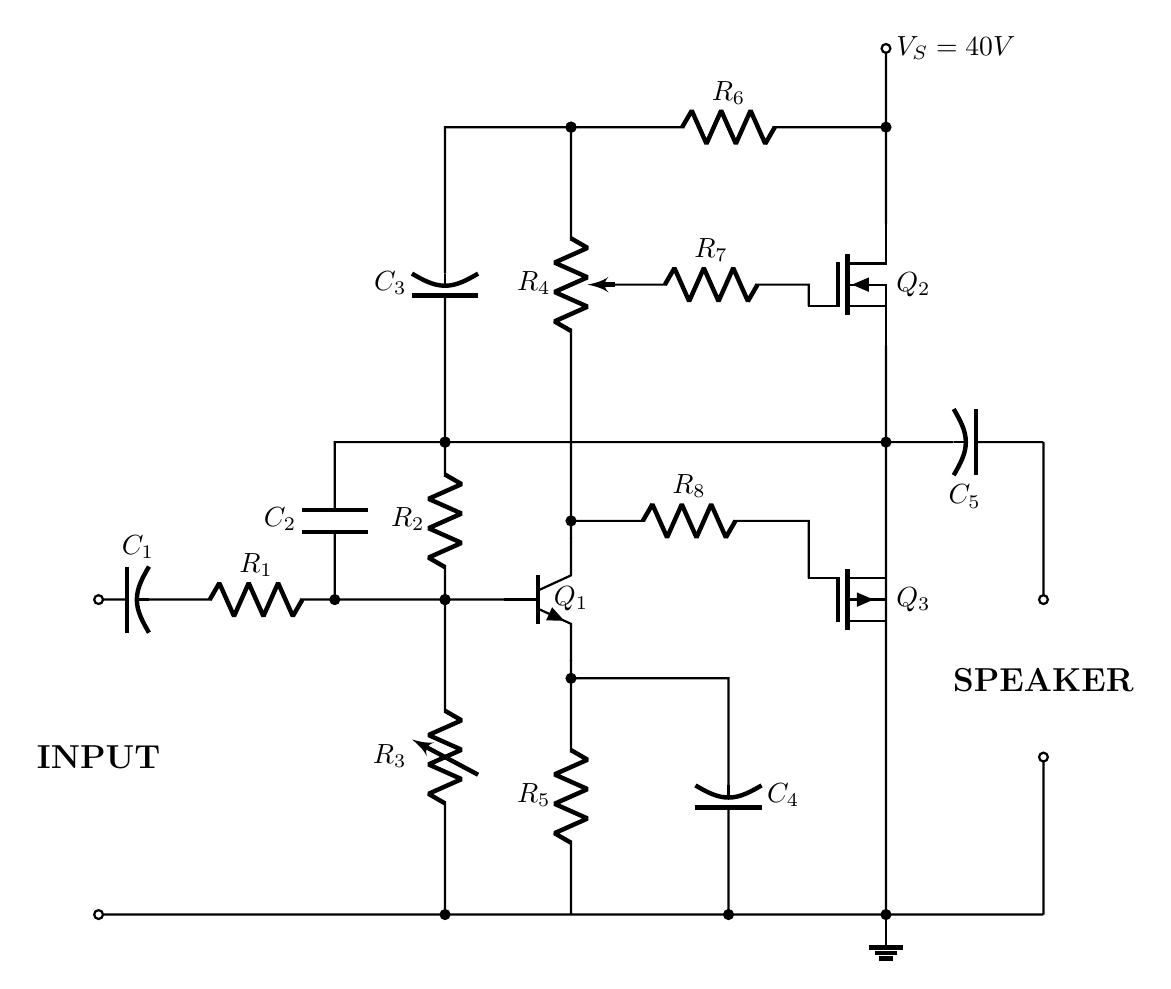
\begin{tikzpicture}[scale=2]
  \draw[color=black, thick]
    (0,0) to [short,o-] (6,0){} % Baseline for connection to ground
    % Input and ground
    (0,1) node[]{\large{\textbf{INPUT}}}
    % Connection of passive components
    (5,0) node[ground]{} node[circ](4.5,0){}
    (0,2) to [cC, l=$C_1$, o-] (0.5,2)
    to [R,l=$R_1$,](1.5,2)
    to node[short]{}(2.6,2)
    (1.5,2) to [C, l=$C_2$, *-] (1.5,3) -| (5,3)
    (2.2,2) to [R, l=$R_2$, *-*] (2.2,3)
    (2.2,3) to [cC, l=$C_3$, *-] (2.2,5) -| (3,5)
    % Transistor Bipolar Q1
    (3,0) to [R,l=$R_5$,-*] (3,1.5)
    to [Tnpn,n=npn1] (3,2.5)
    (npn1.E) node[right=3mm, above=5mm]{$Q_1$} % Labelling the NPN transistor
    (4,0) to [cC, l_=$C_4$, *-] (4, 1.5)--(3,1.5)
    (2.2,0) to [vR, l=$R_3$, *-*] (2.2,2)
    (3,2.5) to node[short]{}(3,3)
    (3,5) to [pR, n=pot1, l_=$R_4$, *-] (3,3)
    (3,5) to [R, l=$R_6$, *-] (5,5)
    to [short,*-o](5,5.5) node[right]{$V_S=40 V$}
    % Mosfet Transistors
    (5,3) to [Tnigfetd,n=mos1] (5,5)
    (mos1.B) node[anchor=west]{$Q_2$} % Labelling MOSFET Q2 Transistor
    (pot1.wiper) to [R, l=$R_7$] (4.5,4) -| (mos1.G)
    (5,1.5) to [Tpigfetd,n=mos2] (5,2.5)
    (5,0) to (mos2.S)
    (3,2.5) to [R, l=$R_8$, *-] (4.5,2.5)
    -| (mos2.G)
    (mos2.B) node[anchor=west]{$Q_3$} % Labelling MOSFET Q3 Transistor
    % Output
    (6,3) to [cC, l=$C_5$,-*](5,3)
    (6,3) to [short,-o] (6,2){}
    (mos1.S)--(mos2.D)
    (6,0) to [short,-o] (6,1){} node[above=7mm]{\large{\textbf{SPEAKER}}}
    ;
\end{tikzpicture}
\end{VerbatimOut}

\MyIO


\begin{VerbatimOut}{z.out}


\section{Kalman Filter System Model}

This Kalman filter system model was done by Burkart Lingner
\cite{lingner2010}.
\ix{Lingner, Burkart}

% An example using TikZ/PGF 2.00
%
% Features: Decorations, Fit, Layers, Matrices, Styles
% Tags: Block diagrams, Diagrams
% Technical area: Electrical engineering

%%%% \documentclass[a4paper,10pt]{article}
%%%% 
%%%% \usepackage[english]{babel}
%%%% \usepackage[T1]{fontenc}
%%%% \usepackage[ansinew]{inputenc}
%%%% 
%%%% \usepackage{lmodern}	% font definition
%%%% \usepackage{amsmath}	% math fonts
%%%% \usepackage{amsthm}
%%%% \usepackage{amsfonts}
%%%% 
%%%% \usepackage{tikz}
%%%% 
%%%% %%%<
%%%% \usepackage{verbatim}
%%%% \usepackage[active,tightpage]{preview}
%%%% \PreviewEnvironment{tikzpicture}
%%%% \setlength\PreviewBorder{5pt}%
%%%% %%%>
%%%% 
%%%% \begin{comment}
%%%% :Title: Kalman Filter System Model
%%%% :Slug: kalman-filter
%%%% :Author: Burkart Lingner
%%%% 
%%%% This is the system model of the (linear) Kalman filter. 
%%%% 
%%%% \end{comment}
%%%% 
%%%% 

\begin{figure}[htbp]
\caption{Kalman filter system model}
\centering
% The state vector is represented by a blue circle.
% "minimum size" makes sure all circles have the same size
% independently of their contents.
\tikzstyle{state}=[circle,
                                    thick,
                                    minimum size=1.2cm,
                                    draw=blue!80,
                                    fill=blue!20]

% The measurement vector is represented by an orange circle.
\tikzstyle{measurement}=[circle,
                                                thick,
                                                minimum size=1.2cm,
                                                draw=orange!80,
                                                fill=orange!25]

% The control input vector is represented by a purple circle.
\tikzstyle{input}=[circle,
                                    thick,
                                    minimum size=1.2cm,
                                    draw=purple!80,
                                    fill=purple!20]

% The input, state transition, and measurement matrices
% are represented by gray squares.
% They have a smaller minimal size for aesthetic reasons.
\tikzstyle{matrx}=[rectangle,
                                    thick,
                                    minimum size=1cm,
                                    draw=gray!80,
                                    fill=gray!20]

% The system and measurement noise are represented by yellow
% circles with a "noisy" uneven circumference.
% This requires the TikZ library "decorations.pathmorphing".
\tikzstyle{noise}=[circle,
                                    thick,
                                    minimum size=1.2cm,
                                    draw=yellow!85!black,
                                    fill=yellow!40,
                                    decorate,
                                    decoration={random steps,
                                                            segment length=2pt,
                                                            amplitude=2pt}]

% Everything is drawn on underlying gray rectangles with
% rounded corners.
\tikzstyle{background}=[rectangle,
                                                fill=gray!10,
                                                inner sep=0.2cm,
                                                rounded corners=5mm]

\begin{tikzpicture}[>=latex,text height=1.5ex,text depth=0.25ex]
    % "text height" and "text depth" are required to vertically
    % align the labels with and without indices.
  
  % The various elements are conveniently placed using a matrix:
  \matrix[row sep=0.5cm,column sep=0.5cm] {
    % First line: Control input
    &
        \node (u_k-1) [input]{$\mathbf{u}_{k-1}$}; &
        &
        \node (u_k)   [input]{$\mathbf{u}_k$};     &
        &
        \node (u_k+1) [input]{$\mathbf{u}_{k+1}$}; &
        \\
        % Second line: System noise & input matrix
        \node (w_k-1) [noise] {$\mathbf{w}_{k-1}$}; &
        \node (B_k-1) [matrx] {$\mathbf{B}$};       &
        \node (w_k)   [noise] {$\mathbf{w}_k$};     &
        \node (B_k)   [matrx] {$\mathbf{B}$};       &
        \node (w_k+1) [noise] {$\mathbf{w}_{k+1}$}; &
        \node (B_k+1) [matrx] {$\mathbf{B}$};       &
        \\
        % Third line: State & state transition matrix
        \node (A_k-2)         {$\cdots$};           &
        \node (x_k-1) [state] {$\mathbf{x}_{k-1}$}; &
        \node (A_k-1) [matrx] {$\mathbf{A}$};       &
        \node (x_k)   [state] {$\mathbf{x}_k$};     &
        \node (A_k)   [matrx] {$\mathbf{A}$};       &
        \node (x_k+1) [state] {$\mathbf{x}_{k+1}$}; &
        \node (A_k+1)         {$\cdots$};           \\
        % Fourth line: Measurement noise & measurement matrix
        \node (v_k-1) [noise] {$\mathbf{v}_{k-1}$}; &
        \node (H_k-1) [matrx] {$\mathbf{H}$};       &
        \node (v_k)   [noise] {$\mathbf{v}_k$};     &
        \node (H_k)   [matrx] {$\mathbf{H}$};       &
        \node (v_k+1) [noise] {$\mathbf{v}_{k+1}$}; &
        \node (H_k+1) [matrx] {$\mathbf{H}$};       &
        \\
        % Fifth line: Measurement
        &
        \node (z_k-1) [measurement] {$\mathbf{z}_{k-1}$}; &
        &
        \node (z_k)   [measurement] {$\mathbf{z}_k$};     &
        &
        \node (z_k+1) [measurement] {$\mathbf{z}_{k+1}$}; &
        \\
    };
    
    % The diagram elements are now connected through arrows:
    \path[->]
        (A_k-2) edge[thick] (x_k-1)	% The main path between the
        (x_k-1) edge[thick] (A_k-1)	% states via the state
        (A_k-1) edge[thick] (x_k)		% transition matrices is
        (x_k)   edge[thick] (A_k)		% accentuated.
        (A_k)   edge[thick] (x_k+1)	% x -> A -> x -> A -> ...
        (x_k+1) edge[thick] (A_k+1)
        
        (x_k-1) edge (H_k-1)				% Output path x -> H -> z
        (H_k-1) edge (z_k-1)
        (x_k)   edge (H_k)
        (H_k)   edge (z_k)
        (x_k+1) edge (H_k+1)
        (H_k+1) edge (z_k+1)
        
        (v_k-1) edge (z_k-1)				% Output noise v -> z
        (v_k)   edge (z_k)
        (v_k+1) edge (z_k+1)
        
        (w_k-1) edge (x_k-1)				% System noise w -> x
        (w_k)   edge (x_k)
        (w_k+1) edge (x_k+1)
        
        (u_k-1) edge (B_k-1)				% Input path u -> B -> x
        (B_k-1) edge (x_k-1)
        (u_k)   edge (B_k)
        (B_k)   edge (x_k)
        (u_k+1) edge (B_k+1)
        (B_k+1) edge (x_k+1)
        ;
    
    % Now that the diagram has been drawn, background rectangles
    % can be fitted to its elements. This requires the TikZ
    % libraries "fit" and "background".
    % Control input and measurement are labeled. These labels have
    % not been translated to English as "Measurement" instead of
    % "Messung" would not look good due to it being too long a word.
    \begin{pgfonlayer}{background}
        \node [background,
                    fit=(u_k-1) (u_k+1),
                    label=left:Entrance:] {};
        \node [background,
                    fit=(w_k-1) (v_k-1) (A_k+1)] {};
        \node [background,
                    fit=(z_k-1) (z_k+1),
                    label=left:Measure:] {};
    \end{pgfonlayer}
\end{tikzpicture}

\end{figure}
\end{VerbatimOut}

\MyIO

%\ProvidesFile{ap-linguistics.tex}[2021-08-23 linguistics appendix]

\begin{VerbatimOut}{z.out}
\chapter{LINGUISTICS}
\ix{linguistics//Linguistics appendix}

See WIKIBOOKS \LaTeX/Linguistics \cite{wikibooks-latex-linguistics}
or google for the information you need.

The doulossil font \cite{tambe2020}
is a TrueType font.
Version 0.1 on September 21, 2020 claimed
``it has characters that are not in other TeX IPA fonts''.
\end{VerbatimOut}

\MyIO

%\ProvidesFile{ap-mathematics.tex}[2021-08-23 mathematics appendix]

\begin{VerbatimOut}{z.out}
\chapter{MATHEMATICS}
\ix{mathematics//Mathematics appendix}

\PurdueThesisLogo\ loads the \AMSmathLogo\ package \cite{amslatex3project2019}
to do mathematics.
\end{VerbatimOut}

\MyIO


\begin{VerbatimOut}{z.out}
There are two types of mathematics in \LaTeX.
Text math is math that that is interspersed with text.
For example, this is text math: \(a = b + c\).
This is display math:
\begin{equation}
  a = b + c
\end{equation}
\end{VerbatimOut}

\MyIO


\begin{VerbatimOut}{z.out}
\newpage

\section{Standard Functions}

Standard functions should be in a roman font.
Like this: \(\cos\theta\).
Here is a list of standard function commands:\\

% The "@{\hspace*{\parindent}}" indents the table
% the same amount as a paragraph.
\begin{tabular}{@{\hspace*{\parindent}}llll@{}}
  \verb+\arccos+& \verb+\csc+& \verb+\ker+&    \verb+\min+\\
  \verb+\arcsin+& \verb+\deg+& \verb+\lg+&     \verb+\Pr+\\
  \verb+\arctan+& \verb+\det+& \verb+\lim+&    \verb+\sec+\\
  \verb+\arg+&    \verb+\dim+& \verb+\liminf+& \verb+\sin+\\
  \verb+\cos+&    \verb+\exp+& \verb+\limsup+& \verb+\sinh+\\
  \verb+\cosh+&   \verb+\gcd+& \verb+\ln+&     \verb+\sup+\\
  \verb+\cot+&    \verb+\hom+& \verb+\log+&    \verb+\tan+\\
  \verb+\coth+&   \verb+\inf+& \verb+\max+&    \verb+\tanh+\\
\end{tabular}
\ix
{%
  arccos//arcsin//arctan//arg//cos//cosh//cot//coth%
  //csc//deg//det//dim//exp//gcd//hom//inf%
  //ker//lg//lim//liminf//limsup//ln//log//max%
  //min//Pr//sec//sin//sinh//sup//tan//tanh%
}
\index{\verb+\arccos+} \index{\verb+\arcsin+} \index{\verb+\arctan+} \index{\verb+\arg+}
\index{\verb+\cos+} \index{\verb+\cosh+} \index{\verb+\cot+} \index{\verb+\coth+}
\index{\verb+\csc+} \index{\verb+\deg+} \index{\verb+\det+} \index{\verb+\dim+}
\index{\verb+\exp+} \index{\verb+\gcd+} \index{\verb+\hom+} \index{\verb+\inf+}
\index{\verb+\ker+} \index{\verb+\lg+} \index{\verb+\lim+} \index{\verb+\liminf+}
\index{\verb+\limsup+} \index{\verb+\ln+} \index{\verb+\log+} \index{\verb+\max+}
\index{\verb+\min+} \index{\verb+\Pr+} \index{\verb+\sec+} \index{\verb+\sin+}
\index{\verb+\sinh+} \index{\verb+\sup+} \index{\verb+\tan+} \index{\verb+\tanh+}
\end{VerbatimOut}

\MyIO


\begin{VerbatimOut}{z.out}
\newpage

\section{English Words in Math}

English words in math should be in a roman font like this:\\
Let the maximum value of \(a\) be \(a_\text{max}\).\\
\(a_\text{max} \ge a_\text{min}\) should always be true.\\
The temperature in the attic is \(t_\text{attic}\).
\end{VerbatimOut}

\MyIO


\begin{VerbatimOut}{z.out}
\section{Text Math}

Use \verb+\(+ to start text math and \verb+\)+ to end text math.
Some people use \verb+$+ to start and end text math---I don't
recommend that because \LaTeX\ can give better error messages
if you use \verb+\(+ and \verb+\)+.
\end{VerbatimOut}

\MyIO


\begin{VerbatimOut}{z.out}
\section{Displayed Equations}

Do not use \verb+$$+ to start or end displayed math like \TeX\ uses
\cite{gratzer2016}.

The \AMSmathLogo\ package provides a number
of additional displayed equation structures
beyond the ones provided in basic \LaTeX.
The augmented set includes \cite{amslatex3project2019b}:

\hbox to\hsize{%
  \hss
  \begin{tabular}{@{}ll@{}}
    \toprule
    \bfseries Environment& \bfseries Used for\\
    \midrule
    \tt equation& used for single equations\\
    \tt multline& split single equations over multiple lines\\
    \tt gather& collect but do not align multiple equations\\
    \tt align& align multiple equations\\
    \tt alignat& aligns multiple equations at multiple places\\
    \tt flalign& aligns multiple equations at multiple places on full length lines\\
    \tt split& split a single equation over multiple lines\\
    \bottomrule
  \end{tabular}%
  \hss
}

All but \verb+split+ can be followed by \verb+*+ to not number equations.
\end{VerbatimOut}

\MyIO


\begin{VerbatimOut}{z.out}

\subsection{\texttt{equation} environment}

The \verb+equation+ environment is used for single equations.

\begin{equation}
  E = mc^2
\end{equation}
\end{VerbatimOut}

\MyIO


\begin{VerbatimOut}{z.out}

The \verb+equation*+ environment does single, unnumbered equations.

\begin{equation*}
  a = b_0c + \frac12 de^2 + {\textstyle \frac12} fg^2
    + h_1 + h_2 + \cdots + h_n
    \qquad \text{for \(c \ne d\) and \(g < \infty\)}
\end{equation*}
\end{VerbatimOut}

\MyIO


\begin{VerbatimOut}{z.out}

\textcite{greene-2021-03-14} wrote
% \begin{quotation}  
  For
  \href{https://twitter.com/hashtag/PiDay?src=hashtag\_click\#PiDay}{\#PiDay},
  one of the coolest formulae for today's honoree:
  \[
    \frac 1\pi
    =
    \frac {\sqrt8} {9801}
    \sum_{n=0}^\infty
    \frac  {(4n!) (1103+26390n)}  {(n!)^4 396^{4n}}
  \]
% \end{quotation}
\end{VerbatimOut}

\MyIO


\begin{VerbatimOut}{z.out}

International standard ISO 80000-2:2019 \cite{iso8000022019}
states that $\mit e$,~$\mit i$,~$\mit j$,
and $\itpi$ should appear as
$e$,~$i$,~$j$
and~$\pi$ because they are constants.
This is done automatically by the pa-mismath package
that is loaded by thesis.tex.
See thesis.tex for more information,
including what to do if you're not using those as constants.

Euler's identity is
\begin{equation*}
  e^{i\pi} + 1 = 0.
\end{equation*}
\end{VerbatimOut}

\MyIO


\begin{VerbatimOut}{z.out}

Here's a simple formula relating $e$,~$i$,~$\pi$, and~$\phi$,
the golden ratio
\begin{equation}
  e^{i\pi} + 2\phi = \sqrt 5.
\end{equation}
I didn't notice anything on the web about putting the symbol for
the golden ratio in a special font even though it is a constant.
\end{VerbatimOut}

\MyIO


\begin{VerbatimOut}{z.out}

International standard ISO 80000-2:2019 \cite{iso8000022019}
states that the ``$d\/$'' in math differentials
should be typeset as ``$\di$''.
So,
\begin{equation*}
  \text{use } \int x\di x\qquad\qquad \text{instead of } \int x\,dx
\end{equation*}
\end{VerbatimOut}

\MyIO


\begin{VerbatimOut}{z.out}

The formula for Bekenstein-Hawking entropy:

\begin{equation*}
  S_\text{BH}
  =
  \frac A {4L_P^2}
  = \frac {c^3A} {4G\hbar}
\end{equation*}
\end{VerbatimOut}

\MyIO


\begin{VerbatimOut}{z.out}

Type in the math and let \LaTeX\ worry about the spacing.
You only need to do fine tuning by hand if it looks bad.

Another \verb+equation*+ environment,
note the spacing before the large close parenthesis:

\begin{equation*}
  \frac ab
    = ab^{-1}
    % Parens are the wrong size.
    = (\sqrt{\frac ab})^2
    % Parens are the right size but closing paren is too close to radical.
    = \left( \sqrt\frac ab \right)^2
    % Parens are right size but a negative thin space puts closing paren on top of radical.
    = \left( \sqrt\frac ab \!\right)^2
    % Parens are right size but a thin space puts closing paren too close to radical.
    = \left( \sqrt\frac ab \,\right)^2
    % Parens are right size but a medium space puts closing paren too close to radical.
    = \left( \sqrt\frac ab \:\right)^2
    % Parens are right size and I think a thick space looks the best.
    = \left( \sqrt\frac ab \;\right)^2
\end{equation*}
\end{VerbatimOut}

\MyIO


\begin{VerbatimOut}{z.out}

\begin{equation*}
  (\cos x)^2 + (\sin x)^2 = \cos^2 x + \sin^2 x = 1
\end{equation*}
\end{VerbatimOut}

\MyIO


\begin{VerbatimOut}{z.out}

\begin{equation}
  x \mod 2 =
  \begin{cases}
    0& \text{if $x$ is even}\\
    1& \text{if $x$ is odd}\\
  \end{cases}
\end{equation}
\end{VerbatimOut}

\MyIO


\begin{VerbatimOut}{z.out}

The first six derivatives of distance are velocity, acceleration, jerk, snap, crackle,
and pop \cite{reid2013}.

\begin{equation}
  % Every array element should be in \displaystyle (a big font).
  \AtBeginEnvironment{array}{\everymath{\displaystyle}}
  % Set space between columns to zero, use {} = ... to add a little space before the = "by hand".
  \arraycolsep = 0pt
  \text{distance derivitives} = \left\{\ %
    \begin{array}{llllllll}
      % I'm formatting the first 4 lines different from the last 3 so this will fit on one page.
      x&      {}=\text{distance}&     {}=vt\\[2pt]
      v&      {}=\text{velocity}&     {}=\frac{\di x}{\di t}\\[9pt]
      a&      {}=\text{acceleration}& {}=\frac{\di v}{\di t}& {}=\frac{\di^2x}{\di t^2}\\[9pt]
      \mit j& {}=\text{jerk}&         {}=\frac{\di a}{\di t}& {}=\frac{\di^2v}{\di t^2}&
        {}=\frac{\di^3x}{\di t^3}\\[9pt]
      s
        & {}=\text{snap}
        & {}=\frac{\di \mit j}{\di t}
        & {}=\frac{\di^2a}{\di t^2}
        & {}=\frac{\di^3v}{\di t^3}
        & {}=\frac{\di^4x}{\di t^4}\\[9pt]
      c
        & {}=\text{crackle}
        & {}=\frac{\di s}{\di t}
        & {}=\frac{\di^2\mit j}{\di t^2}
        & {}=\frac{\di^3a}{\di t^3}
        & {}=\frac{\di^4v}{\di t^4}
        & {}=\frac{\di^5x}{\di t^5}\\[9pt]
      p
        & {}=\text{pop}
        & {}=\frac{\di c}{\di t}
        & {}=\frac{\di^2s}{\di t^2}
        & {}=\frac{\di^3\mit j}{\di t^3}
        & {}=\frac{\di^4a}{\di t^4}
        & {}=\frac{\di^5v}{\di t^5}
        & {}=\frac{\di^6x}{\di t^6}
    \end{array}
  \right.
\end{equation}
\end{VerbatimOut}

\MyIO


\begin{VerbatimOut}{z.out}

\subsection{\texttt{multline} environment}

The \verb+multline+ environment is used
to split single equations over multiple lines.

\begin{multline}
  S = a + b + c + d + e + f + g + h + i + j\\
  + k + l + m + n + o + p\\
  + q + r + s + t + u + v + w + x + y + z
\end{multline}
\end{VerbatimOut}

\MyIO


\begin{VerbatimOut}{z.out}

\begin{multline}
  S = a + b + c + d + e\\
  + f + g + h + i + j\\
  + k + l + m + n + o\\
  + p + q + r + s + t\\
  + u + v + w + x + y\\
  + z
\end{multline}
\end{VerbatimOut}

\MyIO


\begin{VerbatimOut}{z.out}

% Calculate width of space before equation plus equation number.
% (All digits are the same width.)
\newdimen{\tdimen}
\settowidth{\tdimen}{\kern\multlinetaggap (L.5)}
\begin{multline}
  S = a + b + c + d + e\\
  \makebox[\textwidth]{\hfill $+ f + g + h + i + j$\hfill\hfill\hfill\hfill\kern\tdimen}\\
  \makebox[\textwidth]{\hfill\hfill${} + k + l + m + n + o$\hfill\hfill\hfill\kern\tdimen}\\
  \makebox[\textwidth]{\hfill\hfill\hfill${} + p + q + r + s + t$\hfill\hfill\kern\tdimen}\\
  \makebox[\textwidth]{\hfill\hfill\hfill\hfill${} + u + v + w + x + y$\hfill\kern\tdimen}\\
  + z
\end{multline}
\end{VerbatimOut}

\MyIO


\begin{VerbatimOut}{z.out}

\subsection{\texttt{gather} environment}

The \verb+gather+ environment collects but does not align multiple equations.

\begin{gather}
  a = b + c + d + e + f + g + h + i + j + k + l\\
  m = n + o + p + q + r + s + t + u + v + w + x + y + z
\end{gather}
\end{VerbatimOut}

\MyIO


\begin{VerbatimOut}{z.out}

\begin{gather}
  a = b + c + d + e + f + g + h + i + j + k + l\notag\\
  m = n + o + p + q + r + s + t + u + v + w + x + y + z
\end{gather}
\end{VerbatimOut}

\MyIO


\begin{VerbatimOut}{z.out}

\begin{gather*}
  \alpha = \beta + \gamma + \delta + \eta\\
  \theta = \iota + \kappa + \lambda + \mu + \nu + \rho + \tau
\end{gather*}
\end{VerbatimOut}

\MyIO


\begin{VerbatimOut}{z.out}

\begin{gather}
  x_\text{min} + x_\text{max} \le \sum_{i=1}^n x_i\\
  x_\text{min} + x_\text{max}
    = \sum_{i=1}^n x_i - \sum_{i=2}^{n-1} x_i\quad\text{if $x$ is sorted}\\
  x_\text{min} \le \left(\sum_{i=1}^n x_i\right) / n
\end{gather}
\end{VerbatimOut}

\MyIO


\begin{VerbatimOut}{z.out}

\subsection{\texttt{align} environment}

The \verb+align+ environment aligns multiple equations.

\begin{align}
  a &= b + c + d\\
  e &= f + g + h + i + j
\end{align}
\end{VerbatimOut}

\MyIO


\begin{VerbatimOut}{z.out}

\begin{align}
  x = \frac{-b \pm \sqrt{b^2-4ac}}{2a}\notag\\
  % Put a thin space before the b^2 to improve the appearance.
  x = \frac{-b \pm \sqrt{\,b^2-4ac}}{2a}
\end{align}
\end{VerbatimOut}
\ix{align environment}
\index{\verb+\begin{align}+}
\ix{thin space}
\index{\verb+\,+}

\MyIO


\begin{VerbatimOut}{z.out}

Quadratic formula proof \cite{khan}:
\ix{quadratic formula}

% The align environment requires the amsmath package.
% Use \addtolength{\jot}{6pt} to increase the space between rows in an amsmath multi-line math formula.
% That's not done here so everything will fit on one page.
\begin{align}
  ax^2 + bx + c &= 0\\
  ax^2 + bx &= -c\notag\\
  % The "\," adds a thinspace of horizontal space.
  x^2 + \frac ba\,x &= -\frac ca\notag\\
  x^2 + \frac ba\,x + \frac{b^2}{4a^2} &= \frac{b^2}{4a^2} - \frac ca\notag\\
  \left(x + \frac b{2a}\right)^2 &= \frac{b^2}{4a^2} - \frac ca\notag\\
  \left(x + \frac b{2a}\right)^2 &= \frac{b^2}{4a^2} - \frac{4ac}{4a^2}\notag\\
  \left(x + \frac b{2a}\right)^2 &= \frac{b^2-4ac}{4a^2}\notag\\
  \sqrt{\left(x + \frac b{2a}\right)^2}
    &= \sqrt{\left(\frac{b^2-4ac}{4a^2}\right)}\notag\\
  x + \frac b{2a} &= \pm \frac{\sqrt{\,b^2-4ac}}{\sqrt{4a^2}}\notag\\
  x + \frac b{2a} &= \pm \frac{\sqrt{\,b^2-4ac}}{2a}\notag\\
  x &= - \frac b{2a} \pm \frac{\sqrt{\,b^2-4ac}}{2a}\notag\\
  x &= \frac{-b \pm \sqrt{\,b^2-4ac}}{2a}
\end{align}
\end{VerbatimOut}

\MyIO


\begin{VerbatimOut}{z.out}

\subsection{\texttt{alignat} environment}
\index{\verb+\begin{aligo}+@\verb+\begin{alignat}+}
\ix{alignat environment}

The \verb+alignat+ environment aligns multiple equations at multiple places.
\begin{alignat}{2}
  a &= b& \qquad\qquad& \text{set $a$}\\
  c &= d& &             \text{you guessed it, set $c$}\notag\\
  g &= h& &             \text{and finally, set $g$}
\end{alignat}
\index{\verb+\begin{aligo}+@\verb+\begin{alignat}+}
\ix{alignat environment}
  
I like to align input columns on the input if possible
and will sometimes use windows over~250 characters wide to do so.
If that won't work I sometimes do,
for example,
\begin{alignat}{2}
  a
    &= b
    & \qquad\qquad
    & \text{set $a$}\\
  c
    &= d
    &
    &\text{you guessed it, set $c$}\notag\\
  g
    &= h
    &
    &\text{and finally, set $g$}
\end{alignat}
\index{\verb+\begin{aligo}+@\verb+\begin{alignat}+}
\ix{alignat environment}

Do whatever works best for you.

\end{VerbatimOut}

\MyIO


\begin{VerbatimOut}{z.out}

Quadratic formula proof \cite{khan}:

% Make changes to \jot be local to the group that starts on the next line.
{
  % Increase distance between lines by 6pt.
  \addtolength{\jot}{6pt}
  \begin{alignat}{2}
    ax^2 + bx + c
      &= 0
      &
      &\text{subtract $c$}\\
    ax^2 + bx
      &= -c
      &
      &\text{divide by $a$}\notag\\
    % The "\," adds a thinspace of horizontal space.
    x^2 + \frac ba\,x
      &= -\frac ca
      &
      &\text{add $\displaystyle\frac{b^2}{4a^2}$}\notag\\
    x^2+\frac ba\,x+\frac{b^2}{4a^2}
      &= \frac{b^2}{4a^2}-\frac ca
      &
      &\text{factor left hand side}\notag\\
    \left(x+\frac b{2a}\right)^2
      &= \frac{b^2}{4a^2}-\frac ca
      &
      &\text{multiply right-most term by $\displaystyle\frac{4a}{4a}$}\notag\\
    \left(x + \frac b{2a}\right)^2
      &= \frac{b^2}{4a^2}-\frac{4ac}{4a^2}
      &
      &\text{use common denominator}\notag\\
    \left(x + \frac b{2a}\right)^2
      &= \frac{b^2-4ac}{4a^2}
      &
      &\text{take square root of each side}\notag\\
    \sqrt{\left(x + \frac b{2a}\right)^2}
      &= \sqrt{\left(\frac{b^2-4ac}{4a^2}\right)}
      &
      &\text{compute square root of each side}\notag\\
    x + \frac b{2a}
      &= \pm \frac{\sqrt{\,b^2-4ac}}{\sqrt{4a^2}}
      &
      &\text{simplify right hand denominator}\notag\\
    x + \frac b{2a}
      &= \pm \frac{\sqrt{\,b^2-4ac}}{2a}
      &
      &\text{subtract $\displaystyle\frac b{2a}$ from each side}\notag\\
    x
      &= -\frac b{2a} \pm \frac{\sqrt{\,b^2-4ac}}{2a}
      &\qquad
      &\text{use common denominator}\notag\\
    x
      &= \frac{-b \pm \sqrt{\,b^2-4ac}}{2a}
  \end{alignat}
}
\end{VerbatimOut}

\MyIO


\begin{VerbatimOut}{z.out}

\index{\verb+\begin{flalign}+}
\todoindex{Verb+Begin-Ocurly-flalign-Ccurly+}
\ix{falign environment}
\subsection{\texttt{flalign} environment}

The \verb+flalign+ environment aligns multiple equations at multiple places
on full length lines.

\begin{flalign}
  a &= b&   &   & u &= v\\
  c &= d& m &= n& w &= x\notag\\
  g &= h&   &   & y &= z
\end{flalign}
\end{VerbatimOut}

\MyIO


\begin{VerbatimOut}{z.out}

\index{\verb+\begin{split}+}
\todoindex{Verb+Begin-Ocurly-split-Ccurly+}
\ix{split environment}
\subsection{\texttt{split} environment}

The \verb+split+ environment ???.
\end{VerbatimOut}

\MyIO
\index{\verb+\begin{split}+}
\todoindex{Verb+Begin-Ocurly-split-Ccurly+}
\ix{split environment}


\begin{VerbatimOut}{z.out}
\section{Theorem-like environments}

These theorem-like environments are defined
in the amsthm package or in\\  % break line here so we don't go past right margin
\verb+PurdueThesis.cls+.
\end{VerbatimOut}

\MyIO


\begin{VerbatimOut}{z.out}

\index{\verb+\begin{definition}+}
\todoindex{Verb+Begin-Ocurly-definition-Ccurly+}
\ix{definition environment}
\begin{definition}
  This is an example definition.
\end{definition}

\index{\verb+\begin{observation}+}
\todoindex{Verb+Begin-Ocurly-observation-Ccurly+}
\ix{observation environment}
\begin{observation}
  This is an example observation.
\end{observation}

\index{\verb+\begin{proof}+}
\todoindex{Verb+Begin-Ocurly-proof-Ccurly+}
\ix{proof environment}
\begin{proof}
  This is an example proof.
  If \(a = b\) and \(b = c\) then \(a = c\).
\end{proof}

\index{\verb+\begin{proposition}+}
\todoindex{Verb+Begin-Ocurly-proposition-Ccurly+}
\ix{proposition environment}
\begin{proposition}
  This is an example proposition.
\end{proposition}

\index{\verb+\begin{theorem}+}
\todoindex{Verb+Begin-Ocurly-theorem-Ccurly+}
\ix{theorem environment}
\begin{theorem}
  This is an example theorem.
\end{theorem}
\end{VerbatimOut}

\MyIO


\begin{VerbatimOut}{z.out}


\section{Examples}

\subsection{Bayes' Theorem}
\ix{Bayes' Theorem}

Bayes' Theorem \cite{bayes}:
{
  \UndefineShortVerb{\|}
\[
  \text{P}(\text A|\text B)
    % The "\," puts a thin horizontal space there, 1/6 of an "em".
    % An "em" is roughly the width of a lowercase "m".
    = \frac{\text P(\text B|\text A)\,\text P(\text A)}{\text P(\text B)}
\]
}
\end{VerbatimOut}

\MyIO


\begin{VerbatimOut}{z.out}

\subsection{Nicomachus's theorem}
\ix{Nicomachus's theorem}

Nicomachus's theorem \cite{wikipedia-nicomachus} states that
the sum of the first~$n$ cubes is the square of the~$n$th triangular number.
That is,
\[
  1^3 + 2^3 + 3^3 + \cdots + n^3 = (1 + 2 + 3 + \cdots + n)^2.
\]
The same equation may be written more compactly using the mathematical notation for summation:
\[
  \sum_{k=1}^n k^3 = \left(\sum_{k=1}^n k\right)^2.
\]
Also see the diagram on that web page.
\end{VerbatimOut}

\MyIO


\begin{VerbatimOut}{z.out}

\subsection{Prime Number Theorem}
\ix{Prime Number Theorem}

\textcite{li2013} suggested using a functional equation
from the Prime Number Theorem proof
as an example:
\begin{equation}
  \int_1^x
    \sum_{p\le u}
    \left\lfloor\frac{\log u}{\log p}\right\rfloor
    \log p
    \,\text{d}u
    =
    \frac1{2\pi i}
    \int_{c-i\infty}^{c+i\infty}
    \frac{x^{s+1}}{s(s+1)}
    \left(-\frac{\zeta'(s)}{\zeta(s)}\right)
    \text{d}s
\end{equation}
\end{VerbatimOut}

\MyIO


\begin{VerbatimOut}{z.out}

\subsection{Quantum Mechanics}
\ix{Quantum Mechanics}

\textcite{greene-2021-04-04} wrote
\ix{Greene, Brian Randolph}
\begin{quotation}
  Quantum Mechanics in a nutshell:
  A particle goes from here to there
  by sampling every possible trajectory from here to there.

  \[
    \langle x_f,t_f \vert x,t_{\mathit i} \rangle
    =
    \sum_{\text p \in \text{paths}} e^{\mathit iS(\text p) \si{\planckbar}}
  \]
\end{quotation}
\end{VerbatimOut}

\MyIO


%  https://tex.stackexchange.com/questions/96568/how-can-i-align-multiple-cases-environment-simultaneously
\begin{VerbatimOut}{z.out}
\subsection{Question in String Theory / Mass of States / Number Operator}


\textcite{yourlazyphysicist2017} wrote
``I have the following definition of the space-time coordinates'':

\newcommand{\fpt}{{4\pi T}}
\newcommand{\oh}{\frac12}
\newcommand{\snnz}{\sum_{n\ne0}}
\newcommand{\tms}{\tau - \sigma}
\newcommand{\tps}{\tau + \sigma}
\begin{align}
    \text{closed string: }&
        \begin{cases}
            \displaystyle
            X^\mu_R
                = \oh x^\mu
                + \frac1\fpt (\tms) p^\mu
                + \frac i{\sqrt\fpt} \snnz \frac1n \alpha^\mu_n e^{-in(\tms)},\\
            \displaystyle
            X^\mu_L
                = \oh x^\mu
                + \frac1\fpt (\tps) p^\mu
                + \frac i{\sqrt\fpt} \snnz \frac1n \tilde\alpha^\mu_n e^{-in(\tps)}.
        \end{cases}\\[6pt]
    \text{open string: }&
        \begin{cases}
            \displaystyle
            X^\mu_N
                = x^\mu
                + \frac1{\pi T}p^\mu\tau
                + \frac i{\sqrt{\pi T}} \snnz \frac1n \alpha^\mu_n e^{-in\tau} \cos(n\sigma),\\
            \displaystyle
            X^\mu_D
                = x^\mu
                + \frac i{\sqrt{\pi T}} \snnz \frac1n \alpha^\mu_n e^{-in\tau} \sin(n\sigma).
        \end{cases}
\end{align}
\end{VerbatimOut}

\MyIO



% https://www.google.com/url?sa=i&rct=j&q=&esrc=s&source=images&cd=&cad=rja&uact=8&ved=0ahUKEwiSzf370-jmAhXIGs0KHRHyAZQQMwiCASgNMA0&url=https%3A%2F%2Fwww.chegg.com%2Fhomework-help%2Fquestions-and-answers%2Fequations-displacement-atoms-along-linear-chain-d2u-u-m-mass-atoms-c-force-constant-neares-q26052186&psig=AOvVaw1eYq-Q0El0Tbjgbp_Lu2Vv&ust=1578183004388936&ictx=3&uact=3

% M\frac{d^2\mu_n}{dt^2} = C(u_{n_1} - 2u_n + u_{n-1}).

% a^{b} same as a^b     c^{de} f^{g^h} ij^{kl}^{mn}

% superscripts
% subscripts

% operators

%\sum
%\prod

%\alpha
%\beta
%\gamma
%\delta
%\epsilor
%\varepsilon
%\zero
%\eta
%\theta
%\vartheta
%\iota
%\kappa
%\lambda
%\mu
%\nu\xi
%\varrho
%\sigma
%\varsigma
%\tau
%\upsilan
%\pha
%\varphi
%\chi
%\psi
%\omega

%\Gamma
%\Delta
%\Theta
%\Lambda
%\Xi
%\Pi
%\Sigmo
%\Upsilan
%\Phi
%\Psi
%\Omega

%mixed greek and text

%x_min, x_max

%\ldots

%\to

%1 + \frac14 + \frac19 + \cdots = \frac\pi6

%fractions

% frac{\ln x}{\ln\alpha} = log_\alpha x

% \sum_{i=1}^n = 1 + 2 + \cdots + n = \frac{n(n+1)}{2}


% xxxx     \end{verbatim}
% xxxx % Requires \usepackage{amsmath}; use align* for no equation number.
% xxxx \begin{align}
% xxxx   a = {}& b + c\\
% xxxx   x = {}& y + z
% xxxx \end{align}
% xxxx     \vskip\baselineskip
% xxxx     \hrule
% xxxx     \vskip0.5\baselineskip
% xxxx     \filbreak
% xxxx
% xxxx     \begin{verbatim}
% xxxx \[
% xxxx   Z =
% xxxx     \left(
% xxxx       \begin{array}{cc}
% xxxx         a& b\\
% xxxx         c& d
% xxxx       \end{array}
% xxxx     \right)
% xxxx \]
% xxxx     \end{verbatim}
% xxxx \[
% xxxx   Z =
% xxxx     \left(
% xxxx       \begin{array}{cc}
% xxxx         a& b\\
% xxxx         c& d
% xxxx       \end{array}
% xxxx     \right)
% xxxx \]
% xxxx     \vskip\baselineskip
% xxxx     \hrule
% xxxx     \vskip0.5\baselineskip
% xxxx     \filbreak
% xxxx
% xxxx     \begin{verbatim}
% xxxx \begin{equation}
% xxxx   \begin{split}
% xxxx     a = {}& b + c\\
% xxxx       & {} + d + e
% xxxx   \end{split}
% xxxx \end{equation}
% xxxx     \end{verbatim}
% xxxx \begin{equation}
% xxxx   \begin{split}
% xxxx     a = {}& b + c\\
% xxxx       & {} + d + e
% xxxx     \end{split}
% xxxx \end{equation}
% xxxx     \vskip\baselineskip
% xxxx     \hrule
% xxxx     \vskip0.5\baselineskip
% xxxx     \filbreak
% xxxx
% xxxx     \begin{verbatim}
% xxxx \[
% xxxx   (\cos x)^2 + (\sin x)^2 = 1
% xxxx \]
% xxxx     \end{verbatim}
% xxxx \[
% xxxx   (\cos x)^2 + (\sin x)^2 = 1
% xxxx \]
% xxxx     \vskip\baselineskip
% xxxx     \hrule
% xxxx     \vskip0.5\baselineskip
% xxxx     \filbreak
% xxxx
% xxxx     \begin{verbatim}
% xxxx If $X = \cos x$ and $Y = \sin x$ then $X^2 + Y^2 = 1$.
% xxxx     \end{verbatim}
% xxxx If $X = \cos x$ and $Y = \sin x$ then $X^2 + Y^2 = 1$.
% xxxx     \vskip\baselineskip
% xxxx     \hrule
% xxxx     \vskip0.5\baselineskip
% xxxx     \filbreak
% xxxx
% xxxx

%\ProvidesFile{ap-music.tex}[2021-08-23 music appendix]

\begin{VerbatimOut}{z.out}
\chapter{MUSIC}
\ix{music//Music appendix}

To get the following printed music score I did the following steps.
\begin{itemize}
  \item
    Get the ``Example of LilyPond input file''
    from the Wikipedia LilyPond page \cite{wikipedia-lilypond}
    and put it in a \verb+fib.ly+ file.
  \item
    Ran \verb+lilypond fib.ly+ and got the following \verb+fib.pdf+ file:
\end{itemize}
\ix{LilyPond music typesetting software}

\noindent 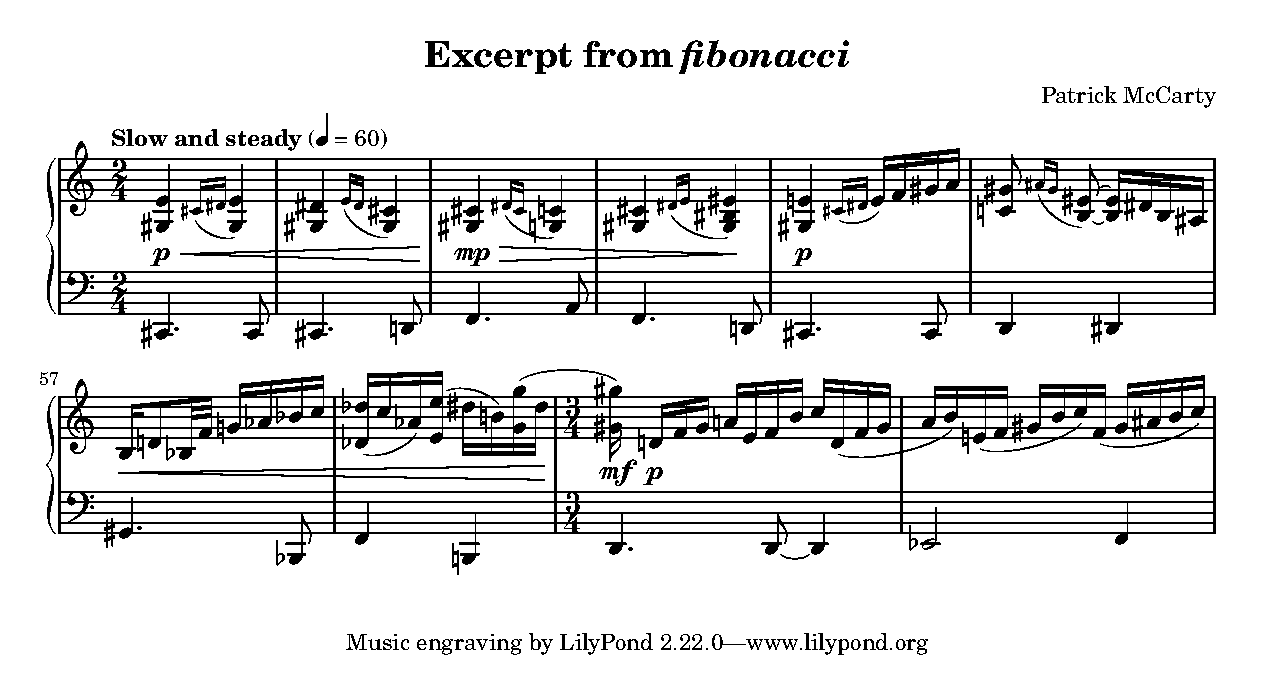
\includegraphics[scale=0.77]{gr-fib.pdf}
\end{VerbatimOut}

\MyIO

% The examples in ap-physics require LuaLaTeX but LuaLaTeX
% screws up the spacing in the List of Figures.  So, the
% ap-physics file is not included.
%
% For some reason, ap-physics doesn't work when using BibTeX.
% Just enclosing \ProvidesFile{ap-physics.tex}[2021-08-23 Physics appendix]

\begin{VerbatimOut}{z.out}
\chapter{PHYSICS}
\ix{physics//Physics appendix}

Feynman diagrams\ix{Feynman diagram}
show what happens
when elementary particles collide
\cite{feynman-diagram}.
The Feynman diagrams below are from the
\citetitle{ellis2016} documentation \cite{ellis2016}.
\textbf{%
  You must use \texttt{lualatex} instead
  of \texttt{pdflatex}
  to process documents that use the \texttt{tikz-feynman} package.%
}

The input
in the documentation
is different than here because a different random number generator
is used \cite{menke2019}.
I expect this to be corrected.
In the meantime try replacing \texttt{vertical}
with \texttt{vertical'}
and/or switch some \texttt{fermion}
to \texttt{anti} \texttt{fermion} lines \cite{ellis2017}.
\end{VerbatimOut}

\MyIO


\begin{VerbatimOut}{z.out}
\feynmandiagram [large, vertical'=e to f] {
  a -- [fermion] b -- [photon, momentum=\(k\)] c -- [fermion] d,
  b -- [fermion, momentum'=\(p_{1}\)] e -- [fermion, momentum'=\(p_{2}\)] c,
  e -- [gluon] f,
  h -- [anti fermion] f -- [anti fermion] i,
};
\end{VerbatimOut}

\MyIO


\begin{VerbatimOut}{z.out}
\feynmandiagram [horizontal=a to b] {
  i1 -- [anti fermion] a -- [anti fermion] i2,
  a -- [photon] b,
  f1 -- [fermion] b -- [fermion] f2,
};
\end{VerbatimOut}

\MyIO
 in braces, i..e.,
%     {
%       \ProvidesFile{ap-physics.tex}[2021-08-23 Physics appendix]

\begin{VerbatimOut}{z.out}
\chapter{PHYSICS}
\ix{physics//Physics appendix}

Feynman diagrams\ix{Feynman diagram}
show what happens
when elementary particles collide
\cite{feynman-diagram}.
The Feynman diagrams below are from the
\citetitle{ellis2016} documentation \cite{ellis2016}.
\textbf{%
  You must use \texttt{lualatex} instead
  of \texttt{pdflatex}
  to process documents that use the \texttt{tikz-feynman} package.%
}

The input
in the documentation
is different than here because a different random number generator
is used \cite{menke2019}.
I expect this to be corrected.
In the meantime try replacing \texttt{vertical}
with \texttt{vertical'}
and/or switch some \texttt{fermion}
to \texttt{anti} \texttt{fermion} lines \cite{ellis2017}.
\end{VerbatimOut}

\MyIO


\begin{VerbatimOut}{z.out}
\feynmandiagram [large, vertical'=e to f] {
  a -- [fermion] b -- [photon, momentum=\(k\)] c -- [fermion] d,
  b -- [fermion, momentum'=\(p_{1}\)] e -- [fermion, momentum'=\(p_{2}\)] c,
  e -- [gluon] f,
  h -- [anti fermion] f -- [anti fermion] i,
};
\end{VerbatimOut}

\MyIO


\begin{VerbatimOut}{z.out}
\feynmandiagram [horizontal=a to b] {
  i1 -- [anti fermion] a -- [anti fermion] i2,
  a -- [photon] b,
  f1 -- [fermion] b -- [fermion] f2,
};
\end{VerbatimOut}

\MyIO

%     }
% doesn't help so it is only loaded if we are using BibLaTeX.
\ifthen{\equal{\bibprocessor}{biblatex}}
{
  \ProvidesFile{ap-physics.tex}[2021-08-23 Physics appendix]

\begin{VerbatimOut}{z.out}
\chapter{PHYSICS}
\ix{physics//Physics appendix}

Feynman diagrams\ix{Feynman diagram}
show what happens
when elementary particles collide
\cite{feynman-diagram}.
The Feynman diagrams below are from the
\citetitle{ellis2016} documentation \cite{ellis2016}.
\textbf{%
  You must use \texttt{lualatex} instead
  of \texttt{pdflatex}
  to process documents that use the \texttt{tikz-feynman} package.%
}

The input
in the documentation
is different than here because a different random number generator
is used \cite{menke2019}.
I expect this to be corrected.
In the meantime try replacing \texttt{vertical}
with \texttt{vertical'}
and/or switch some \texttt{fermion}
to \texttt{anti} \texttt{fermion} lines \cite{ellis2017}.
\end{VerbatimOut}

\MyIO


\begin{VerbatimOut}{z.out}
\feynmandiagram [large, vertical'=e to f] {
  a -- [fermion] b -- [photon, momentum=\(k\)] c -- [fermion] d,
  b -- [fermion, momentum'=\(p_{1}\)] e -- [fermion, momentum'=\(p_{2}\)] c,
  e -- [gluon] f,
  h -- [anti fermion] f -- [anti fermion] i,
};
\end{VerbatimOut}

\MyIO


\begin{VerbatimOut}{z.out}
\feynmandiagram [horizontal=a to b] {
  i1 -- [anti fermion] a -- [anti fermion] i2,
  a -- [photon] b,
  f1 -- [fermion] b -- [fermion] f2,
};
\end{VerbatimOut}

\MyIO

}

% Frequently Asked Questions
%\ProvidesFile{ap-frequently-asked-quetions.tex}[2021-08-23 Frequently Asked Questions appendix]

\begin{VerbatimOut}{z.out}
\chapter{FREQUENTLY ASKED QUESTIONS}
\ix{frequently asked questions//Frequently Asked Questions appendix}

{\bfseries PART OF THESIS WITH PROBLEM}

{
  \def\part#1%
  {
    \vspace*{\baselineskip}
    {\bfseries #1}
  }

  \def\qa#1#2%
  {
    \vspace*{\baselineskip}
    {\small\bfseries Q}: #1\endgraf
    \vspace*{0.5\baselineskip}
    {\small\bfseries A}: #2\endgraf
  }


  \part{Entire Thesis}

  \qa
  {What \LaTeX\ comand should I use to compile my thesis?}
  {%
    The \LuaLaTeXLogo%
    \ix{LuaLaTeX//lualatex}%
    \index{\LuaLaTeXLogo}
    program in the \TeXLiveLogo%
    \index{\TeXLiveLogo}%
    \ix{TeX Live}
    software distribution.
    Overleaf \cite{overleaf}
    (run \LaTeX%
    \index{\LaTeX}
    over the web)
    uses \TeXLiveLogo---%
    in Overleaf click {\tt Menu\/} key in upper left corner of window
    and set {\tt Compiler\/} to {\tt LuaLaTeX} to run \LuaLaTeXLogo.)
    \TeXLiveLogo\ runs on Linux\ix{Linux},
    MacOS\ix{MacOS},
    Unix\ix{Unix},
    and Windows\ix{Windows}.%
  }


  \part{References}

  \qa
  {URLs are not getting printed.  What should I do?}%
  {Make sure you are processing your docuent with \LuaLaTeXLogo.}
}
\end{VerbatimOut}

\MyIO


% Notes and footnotes are optional.
% Reference: TM2017 page 34.
% I have not implemented this yet.  Mark Senn 2002-06-03

% A vita is optional for masters theses
% and required for doctoral dissertations.
% Reference: TM2017 page 13.
% CHANGE NEXT LINE?
%\ProvidesFile{ap-vita.tex}[2021-08-23 vita appendix]

\begin{vita}
\ix{vita}
\index{\verb+\begin{vita}+}
  
[Put a brief autobiographical sketch here.]

\end{vita}


% Listing or including publications(s) is optional.
\ProvidesFile{ap-publications.tex}[2021-08-23 publications appendix]

\ZZnonchapter{odd}{PUBLICATION(S)}{y}{0pt}
\ix{publication,publications}
\index{\verb+\begin{publicationa}+@\verb+\begin{publication}+}
\index{\verb+\begin{publications}+}
    
The following is based on information in
\cite{template1,template2,template3}.

\renewcommand{\I}{\hspace*{2\ZZparindent}$\bullet$\hspace*{1.5em}}

In a publication or publications section you can\\
  \I list a single publication\index{publication}\\
  \I include a single publication\index{publications}\\
  \I list multiple publications\\
  \I include multiple publications\\
Use\newline
\hspace*{0.5in}\verb+\begin{publication}+\ldots\verb+\end{publication}+\newline
or\newline
\hspace*{0.5in}\verb+\begin{publications}+\ldots\verb+\end{publications}+\newline
to skip to the next page and put the appropriate heading on the
top of the page.

\vspace*{1.5\baselineskip}

\section*{To List a Single Publication}

\begin{verbatim}
  \begin{publication}
    ...list a single publication here...
    ...IMPROVE THIS LATER to show how to do that...
  \end{publication}
\end{verbatim}


\section*{To Include a Single Publication}

\begin{verbatim}
  \begin{publication}
    ...put a single publication here...
    ...IMPROVE THIS LATER to show how to do that...
  \end{publication}
\end{verbatim}


\section*{To List Multiple Publications}

\begin{verbatim}
  \begin{publications}
    ...list multiple publications here...
    ...IMPROVE THIS LATER to show how to do that...
  \end{publications}
\end{verbatim}


\section*{To Include Multiple Publications}

\begin{verbatim}
  \begin{publications}
    ...put the multiple publications here...
    ...IMPROVE THIS LATER to show how to do that...
  \end{publications}
\end{verbatim}


% Print the index.
% An index is optional.
\pdfbookmark{INDEX}{index}
\printindex

% Print the colophon.
\ProvidesFile{ap-colophon.tex}[2021-08-23 colophon]

\begin{VerbatimOut}{z.out}
\chapter*{COLOPHON}
\label{ap:colophon}

\ix{colophon}

This is the colophon.

\end{VerbatimOut}

\MyIO


% LaTeX won't read after the \end{document} command.
% You can put notes to yourself or LaTeX input not
% ready for use after "\end{document}" if you'd like.
\end{document}
